\documentclass{ufla}
\usepackage[portuges]{babel}
\usepackage[allbordercolors={1 1 1}, bookmarks=true, bookmarksnumbered=true]{hyperref}
\usepackage[utf8]{inputenc}
\usepackage[cmex10]{amsmath}
\usepackage{ae}
\usepackage{multirow}
\usepackage{rotating}
\usepackage{color}
\usepackage{listings}
\usepackage{tabularx}
% \usepackage[alf,abnt-etal-cite=3,abnt-etal-list=0,abnt-etal-text=emph,bibjustif,abnt-repeated-title-omit=yes,abnt-show-options=warn]{abntex2cite}
\usepackage[alf,abnt-etal-cite=3,abnt-etal-list=0,abnt-etal-text=default,bibjustif,abnt-repeated-title-omit=yes]{abntex2cite} 
\usepackage{pslatex}
\usepackage{amsmath}             % pacote da AMS para Matemática Avançada
\usepackage{amssymb}             % símbolos extras da AMS
\usepackage{latexsym}            % símbolos extras do LaTeX
\usepackage{graphicx}            % para inserção de gráficos
\usepackage{listings}            % para inserção de código
\usepackage{fancyvrb}            % para inserção de saídas de comandos
\usepackage[vlined,linesnumbered,titlenumbered,portuguese]{algorithm2e}
%\usepackage[algoruled, longend, lined,linesnumbered,portuguese]{algorithm2e}
\usepackage{babel}
\usepackage{epsfig}
\usepackage{enumitem}
\usepackage{float}
\usepackage{mathrsfs}
\usepackage{amsfonts}
\usepackage{wasysym}
\usepackage{colortbl} % frescuras em tabelas
\usepackage{babel}
\usepackage{cancel}
\usepackage{scalefnt}
\usepackage{tabularx}
% \usepackage[bottom=3cm,top=3cm,left=3cm,right=3cm]{geometry}
% Configuracao do listings
\lstset{ %
language=C++,                % choose the language of the code
basicstyle=\small\ttfamily,       % the size of the fonts that are used for the code
numbers=left,                   % where to put the line-numbers
numberstyle=\small,      % the size of the fonts that are used for the line-numbers
stepnumber=1,                   % the step between two line-numbers. If it is 1 each line will be numbered
numbersep=1ex,                  % how far the line-numbers are from the code
backgroundcolor=\color{white},  % choose the background color. You must add \usepackage{color}
showspaces=false,               % show spaces adding particular underscores
showstringspaces=false,         % underline spaces within strings
showtabs=false,                 % show tabs within strings adding particular underscores
frame=single,           % adds a frame around the code
tabsize=2,          % sets default tabsize to 2 spaces
captionpos=t,           % sets the caption-position to bottom
breaklines=true,        % sets automatic line breaking
breakatwhitespace=false,    % sets if automatic breaks should only happen at whitespace
keywordstyle=\color[rgb]{0,0,1},
commentstyle=\color[rgb]{0.133,0.545,0.133},
stringstyle=\color[rgb]{0.627,0.126,0.941}
}
\newcommand{\defs}[1]{\textsl{#1}}

\author{Frederico Santos de Oliveira}
\title{Uma avaliação de movimento de malhas baseado na formulação laplaciana na resolução da equação do calor por discretizações de volumes finitos com refinamento de Delaunay}
%\folhaaprovacao{Img/folha-de-aprovacao.pdf}
\date{2014}
\tipo{Dissertação apresentada à Universidade Federal de Lavras, como parte das exigências do Programa de Pós-Graduação em Ciência da Computação, área de concentração em Inteligência Computacional e Processamento Gráfico, para a obtenção do título de Mestre.}
\areaconcentracao{Inteligência Computacional e Processamento Gráfico}

\orientador{Prof. D.Sc. Sanderson L. Gonzaga de Oliveira}
% \coorientador{Dr. Raphael Winckler de Bettio}
% \coorientadorbanca{Dr. Raphael W. de Bettio}
% \coorientadorbancainst{UFLA}
\bancaum{D.Sc. Daniel Furtado Ferreira}
\bancauminst{UFLA}
\bancadois{Ph.D. João Manuel R. S. Tavares}
\bancadoisinst{FEUP}
\defesa{}
\palchaves{Geração de Malhas; Refinamento Adaptativo; Malhas Móveis}
\keywords{Meshes Generation; Adaptive Refinement; Moving Meshes}


% Dados para ficha catalográfica
\fcautor{Oliveira, Frederico Santos de.}
\fcorientador{Sanderson L. Gonzaga de Oliveira}
% Tipo de material para ficha catalográfica
\fctipo{Dissertação (mestrado) -- Universidade Federal de Lavras, 2014.}
% dados para ficha catalográfica 
\fccatalogacao{1. À preencher. 2. À preencher. 3. À preencher. 4. À preencher. I. Universidade Federal de Lavras. II. Título.}
% classificação de acordo com a CDD
\fccdd{CDD -- 000.0}


\hyphenation{Ciência Computação Colegiado Curso Bacharel Universidade Federal Lavras Graduação Inteligência Computacional Processamento Gráfico}

% Aumente este numero para aumentar o espacamento no sumário
% entre os numeros das secoes e os titulos. Este é um fator
% multiplicativo, 1.5 significa uma vez e meia o espaco padrao.
\scalenumwidth{1}

\begin{document}

\maketitle

\pagestyle{empty}
% \dedic{
% Dedico esta dissertação à ...
% }
% 
% \thanks{
% Agradeço a...
% }

\resumo{
Neste trabalho, realiza-se a aplicação de um esquema, combinando o refinamento de delaunay e malhas móveis por volumes finitos na solução da equação do calor. Utiliza-se o algoritmo de \citeonline{Green1978} para geração da malha inicial, o algoritmo de \citeonline{Ruppert1995} para realizar o refinamento adaptativo e o algoritmo de \citeonline{Ungor2004, Ungor2009} para realizar melhorias na qualidade da malha. Movimenta-se os vértices para regiões de grande variação por meio de uma nova função monitora proposta, baseada na suavização laplaciana, que é responsável por guiar o movimento dos vértices. Compara-se a função monitora proposta com outras quatro funções monitoras, também baseadas na suavização laplaciana, presentes na literatura. Os resultados comparativos mostram que a nova função monitora proposta, mesmo não demandando o menor esforço computacional em relação às demais, apresenta a menor quantidade final de vértices. Todos os procedimentos para realização dos experimentos são detalhados ao longo deste trabalho.
}

\resumoingles{
In this paper we apply a scheme, combining the refinement and delaunay meshing in finite volume solution of the heat equation. We use the algorithm \citeonline{Green1978} to generate the initial mesh, the algorithm \citeonline{Ruppert1995} to perform adaptive refinement algorithm and \citeonline{Ungor2004, Ungor2009} to make improvements on mesh quality. We move the vertices to great variability regions using a new proposed monitoring function based on the Laplacian smoothing, which is responsible for guiding the movement of the vertices. We compare the new proposed monitoring function with four other monitor functions, also based on the Laplacian smoothing that we find in the literature. The comparative results show that the new proposed monitoring function, while not requiring the least computational effort compared to the others, has the lowest amount of end vertices. All procedures for the experiments are detailed throughout this work.
}

\listoffigures
\listoftables
\listofacronyms{
	\item[AMR] {\it Adaptive mesh refinement}
        \item[CER] {\it Circunradius-to-shortest edge radio}
        \item[CMr] Cuthill-McKee reverso 
	\item[EDP] Equação diferencial parcial
	\item[FEUP] Faculdade de Engenharia Universidade do Porto
	\item[GMP] {\it GNU Multiple-Precision Library}
	\item[KHI] Instabilidade de Kelvin-Helmholtz 
	\item[MGC] Método dos gradientes conjugados
	\item[MHD] Magneto-hidrodinâmicos 
	\item[MPFR] {\it Multiple-Precision Floating-point computations with correct Rounding}
	\item[MVF] Método dos volumes finitos		
	\item[PE] Princípio de equidistribuição
	\item[PSLG] {\it Planar Straight Line Graph} 
	\item[SPH] {\it Smoothed particle hydrodynamics}
	\item[SRQ] {\it Shape Regularity Quality}
	\item[UFLA] Universidade Federal de Lavras
	\item[VC]  Volume de controle
	\item[VPH] Partículas de Voronoi hidrodinâmicas	
}
\tableofcontents

\pagestyle{ufla}

% As secoes podem estar separadas em arquivos .tex
\section{INTRODUÇÃO}

Técnicas de simulação computacional são utilizadas para descrever diversos fenômenos físicos que são modelados por equações diferenciais parcais (EDPs). Avanços nessas técnicas e o desenvolvimento de computadores de alto desempenho permitiram que fossem aplicadas em diferentes áreas, como o escoamento de fluidos, aerodinâmica, condução térmica, reações químicas, combustão e eletromagnetismo entre outros. Muitas vezes, a complexidade dos modelos que descrevem esses fenômenos torna impraticável o desenvolvimento de soluções analíticas. Desse modo, deve-se recorrer a simulações numéricas, que constituem ferramentas eficientes para solucionar esses problemas. No entanto, para simulação de problemas de grande dimensão, as técnicas numéricas utilizadas devem ser suficientemente eficientes de modo a possibilitarem resultados precisos em tempo viável.

É comum o uso de métodos numéricos, como o método dos elementos finitos e o método dos volumes finitos, que realizam a decomposição do domínio em formas geométricas chamadas, respectivamente, elementos ou volumes de controle. Suas formas variam de tetraedros ou triângulos a quadriláteros, prismas, pirâmides ou hexaedros. Segundo \citeonline{Oliveira2013}:

\begin{quotation} 
A solução aproximada por meio de um método numérico é obtida para um número discreto de pontos, com um determinado erro, proveniente da aproximação e, se o método for convergente, conforme aumenta-se a quantidade de pontos, melhora-se a solução aproximada. A malha pode ser considerada o domínio discretizado geometricamente.
\end{quotation}

De acordo com \citeonline{Oliveira2013}, EDPs que modelam fenômenos físicos frequentemente possuem grandes variações na solução, ou ainda envolvem domínios de geometria complexa, ocasionando erros na solução. Uma estratégia utilizada para se diminuir esses erros é realizar o refinamento da malha. Entretanto, ainda segundo \citeonline{Oliveira2013}, ``ao se utilizar uma malha fina e uniforme ao longo de todo o domínio, tem-se também o aumento do custo computacional, como consequência do aumento do número de pontos.'' Uma forma de se contornar esse problema é posicionar mais pontos nas regiões de grande variação e menos pontos nas regiões de pequena variação, realizando o refinamento adaptativo, ocorrendo uma economia do custo computacional e uma melhoria da solução gerada. 

Dentre os principais aspectos levados em consideração nas técnicas de geração de malhas, destacam-se o tempo de processamento para geração e a qualidade da malha gerada. O tempo de processamento depende da discretização do domínio e, consequentemente, da quantidade de pontos dessa discretização. Já a qualidade, leva em consideração a quantidade, a forma e a distribução dos elementos da malha. A qualidade da malha influencia diretamente nos resultados, tanto nos aspectos visuais quanto no erro da solução. Malhas triangulares tendem a melhor se adaptar ao domínio da solução. Devido a isso, diversas pesquisas de geração e refinamento de malhas vêm sendo realizadas ao longos dos anos. Algumas são brevemente analisadas nos capítulos seguintes deste trabalho.

Também existem várias pesquisas relacionadas às técnicas de adaptatividade de malhas, e algumas delas são citadas neste trabalho, focadas na adaptatividade por refinamento e por movimento dos vértices. Nas técnicas de adaptatividade por refinamento, são inseridos novos pontos nas regiões de interesse. Nas técnicas de adaptatividade por movimento, chamadas de malhas móveis, mantém-se a quantidade original de pontos e realiza-se a realocação destes. Como a inclusão de pontos aumenta o custo computacional, neste trabalho há uma descrição das técnicas de adaptatividade de malhas com foco em malhas móveis.

\subsection{Objetivos}

A seguir serão apresentados o objetivo geral e os específicos deste trabalho.

\subsubsection{Objetivo geral}

Este trabalho tem o objetivo geral de aplicar um esquema que combine o refinamento de Delaunay e malhas móveis por volumes finitos na solução de equações diferenciais parciais de segunda ordem, como a equação de condução do calor.

\subsubsection{Objetivos específicos}

Os objetivos específicos principais são: revisar os conceitos de geração de malhas para resolução de EDPs utilizando o método dos volumes finitos; revisar técnicas de adaptatividade por inclusão de pontos e por malhas móveis; implementar um algoritmo híbrido de refinamento de Delaunay para a geração da malha inicial; gerar e implementar uma técnica de movimento de malhas que combine simplicidade, eficiência e velocidade; realizar experimentos computacionais para comparar os resultados com soluções encontradas na literatura.

\subsection{Organização deste trabalho}

Este trabalho está organizado em cinco capítulos. No capítulo (\ref{cap:referencial_teorico}), elucida-se o referencial teórico para desenvolvimento deste trabalho. Nesse capítulo, apresenta-se a triangulação de Delaunay e o seu dual, o diagrama de Voronoi; a discretização da equação do calor, utilizando-se o método dos volumes finitos com o diagrama de Voronoi; a construção do método dos gradientes conjugados, com pré-condicionamento e reordenação da matriz de coeficientes; e, por fim, aborda-se a suavização laplaciana e as principais características sobre malhas móveis.

No capítulo (\ref{cap:desenvolvimento}), tem-se os detalhes da implementação deste trabalho. Descreve-se o procedimento de refinamento adaptativo e o procedimento que realiza o movimento dos vértices por meio de pseudocódigos. No capítulo (\ref{cap:resultados}), expõe-se os resultados dos experimentos realizados, conforme demonstrado no capítulo que o antecede. 

Finalizando este trabalho, no capítulo (\ref{cap:conclusao}), apresenta-se a conclusão acerca dos resultados dos experimentos, bem como sugestões de trabalhos futuros.
\section{REFERENCIAL TEÓRICO}
\label{cap:referencial_teorico}

Neste capítulo é apresentado o referencial teórico para desenvolvimento deste trabalho. Descreve-se a triangulação de Delaunay e o seu dual, o diagrama de Voronoi, na seção (\ref{cap_triangulacao_delaunay}). Também apresenta-se, nessa seção, algoritmos para geração, manutenção e refinamento de malhas de Delaunay.

Na seção (\ref{cap_discretizacao_equacao_calor}), realiza-se a discretização da equação do calor, utilizando-se o método dos volumes finitos com o diagrama de Voronoi e define-se um algoritmo em forma de pseudocódigo referente a essa discretização. 

Na seção (\ref{cap_metodo_gradientes_conjugados}), tem-se a construção do método dos gradientes conjugados, apresentando-se um pseudocódigo. Com o intuito de se diminuir o número de iterações, também expõe-se nessa seção uma forma de pré-condicionamento da matriz de coeficientes e um algoritmo para reordenação dos vértices, o algoritmo de Cuthill-McKee reverso em conjunto com o algoritmo de vértice pseudoperiférico.

Na seção (\ref{cap_suavizacao_laplaciana}), descreve-se a suavização laplaciana. Também são apresentadas técnicas de melhoria da qualidade da malha utilizando a suavização laplaciana.

Na seção (\ref{cap_malhas_moveis}), aborda-se as principais características sobre malhas móveis, como adaptatividade de malhas, o princípio de equidistribuição, também apresentando diferentes trabalhos que pretendem solucionar equações diferenciais parciais por diferentes métodos, utilizando os mais variados tipos de malhas. Também apresentam-se técnicas de movimento dos vértices baseadas na formulação laplaciana.

Na seção (\ref{cap_metrica_geometrica}), explana-se uma métrica geométrica para verificar a degeneração da malha ao movimentar os vértices.

\subsection{A triangulação de Delaunay e o diagrama de Voronoi}
\label{cap_triangulacao_delaunay}

Nesta seção, aborda-se a triangulação de Delaunay e o diagrama de Voronoi. Também são apresentados algoritmos de construção, manutenção e refinamento dessa triangulação.

\subsubsection{Considerações iniciais}

Uma malha pode ser classificada de acordo com a disposição relativa dos diferentes elementos existentes. Uma malha {\it estruturada} é caracterizada pela sua conectividade {\it regular}. Isso significa que, a posição dos nós pode ser mapeada de modo a definir quais nós serão vizinhos por meio de cálculo. Isso pode restringir as escolhas dos elementos para quadriláteros em 2D ou hexaedros em 3D. Se os nós não podem ser arranjados de tal forma, a malha é dita {\it não estruturada} ou {\it irregular}. Em uma malha irregular, deve-se armazenar a conexão entre os nós que formam a malha. Os elementos podem ser, em sua forma básica, triângulos ou tetraedros em 2D e 3D, respectivamente, bem como hexaedros, ou qualquer outra forma, em malhas mais complexas. \cite[p.~20]{Thompson1999}.

Na busca de se atingir uma determinada qualidade na aproximação, com desempenho computacional aceitável, ao longo das últimas décadas, pesquisas têm sido realizadas em técnicas de geração e refinamento de malhas, como por exemplo em \citeonline{Preparata1985, Thompson1999, Teng2000, Chen2004, George2008}. Ainda em problemas com domínios com geometria complexa, a geração da malha pode ser uma tarefa dispendiosa. Uma forma de se obter uma malha de qualidade a baixo custo computacional é a utilização da triangulação Delaunay. 

A triangulação de \citeonline{Delaunay1939} é um tipo de malha irregular. Com uma triangulação de Delaunay, maximiza-se o menor ângulo da triangulação. Obtém-se triângulos com ângulos não próximos a $0^{\circ}$ e a $180^{\circ}$. Em esquemas numéricos, triângulos com ângulos próximos a $0^{\circ}$ e $180^{\circ}$ são considerados de má qualidade, levando a resultados imprecisos. 

A triangulação de Delaunay possui a característica de unicidade, de forma que, dado um conjunto de vértices, a triangulação é sempre única, exceto em casos degenerados, nos quais quatro ou mais vértices são cocirculares, existindo duas possibilidades de triangulação (local). Cada uma das duas possibilidades de triangulação que divide o quadrilátero em dois triângulos satisfaz a ``condição Delaunay'', isto é, em que o circuncírculo (único círculo que passa pelos vértices do triângulo) é vazio. Essa noção pode ser estendida a três dimensões.

Um diagrama de \citeonline{Voronoi1908} é uma decomposição (em partições) de um espaço em torno de um vértice. Cada polígono consiste em uma região de espaço que fica mais próxima de cada vértice do que qualquer outro vértice gerador do diagrama de Voronoi, que é formado pelos polígonos de Voronoi. Diversos algoritmos para a geração do diagrama de Voronoi foram desenvolvidos. São exemplos desses algoritmos, \citeonline{Shamos1975}, que desenvolveram um algoritmo O($n\cdot \mbox{lg}(n)$) por divisão-e-conquista e \citeonline{Green1978}, que produziram um algoritmo O($n^2$) por inserção incremental, em que $n$ é a quantidade de vértices da triangulação.

Uma partição do diagrama de Voronoi e a triângulação de Delaunay correspondente pode ser observada na figura (\ref{fig_malha_voronoi}).

\begin{figure}[!ht]
  \centering
  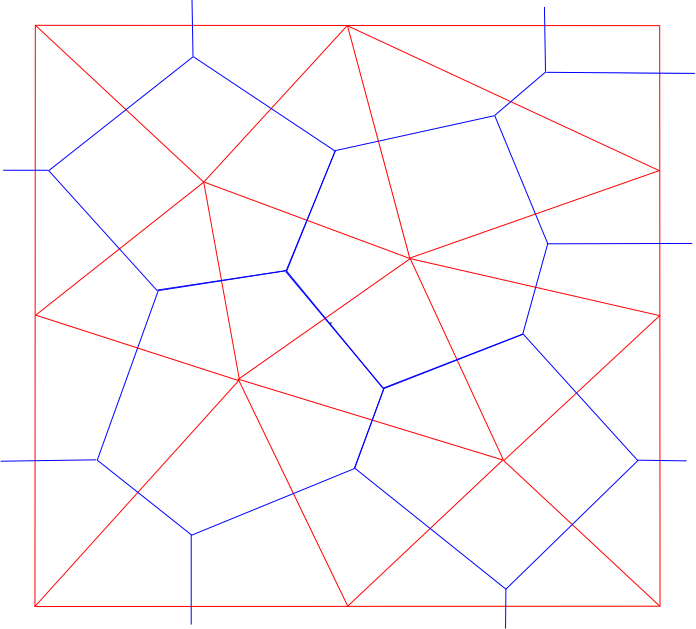
\includegraphics[width=150pt]{imagens_discretizacao/malha_voronoi.png}
  \caption{\footnotesize{Em azul, arestas de uma partição do diagrama de Voronoi e, em vermelho, os triângulos de Delaunay correspondentes.
}}
  \label{fig_malha_voronoi}
\end{figure}

\subsubsection{Manutenção da triangulação de Delaunay - Algoritmo de Lawson}
\label{cap_algoritmo_lawson}
Para construção da triangulação Delaunay, pode-se utilizar o algoritmo de \citeonline{Lawson1977}, um algoritmo de complexidade $O(n^2)$. Esse algoritmo é utilizado para gerar ou para manter uma triangulação de Delaunay. Sua escolha deve-se à sua facilidade de implementação.

A partir de uma triangulação inicial, verifica-se se todas as arestas que compõem a triangulação atendem aos critérios da triangulação de Delaunay. Caso essas arestas não atendam aos critérios da triangulação de Delaunay, realiza-se o {\it flip}. 

O {\it flip} é um procedimento, definido por \citeonline{Lawson1977}, em que ocorre a inversão da aresta invadida, conforme demonstrado na figura (\ref{fig_flip}). Com o {\it flip}, uma nova aresta é criada e, em seguida, verifica-se, recursivamente, essa aresta e os dois triângulos que a compartilham. O algoritmo termina quando todas as arestas atendem aos critérios da triangulação de Delaunay, ou seja, são localmente de Delaunay.  

\begin{figure}[!ht]
  \centering
  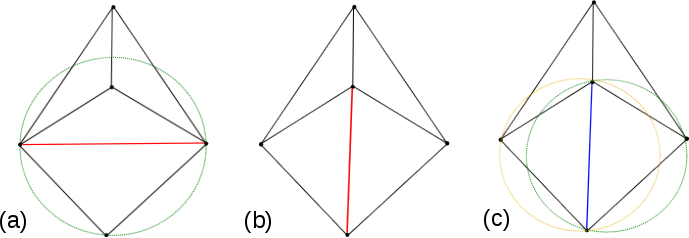
\includegraphics[width=350pt]{imagens_delaunay/novo_flip.png}
  \caption{\footnotesize{Aplicação do algoritmo de Lawson: (a) Uma aresta invadida, mostrada em vermelho, que não é de Delaunay, é verificada. (b) O algoritmo do {\it flip} é aplicado para inverter a aresta invadida, tornando-a localmente de Delaunay. (c) Verifica-se se essa aresta e os dois triangulos que a compartilham são localmente de Delaunay. Como a aresta não é invadida, essa é mostrada em azul.
}}
  \label{fig_flip}
\end{figure}

No algoritmo (\ref{algoritmo_lawson}) tem-se um pseudocódigo referente ao algoritmo de \citeonline{Lawson1977}.

\begin{algorithm}[!ht]
\caption{Algoritmo de Lawson.} 
\label{algoritmo_lawson}
\Entrada{Triangulação $T$.}
\Saida{Triangulação de Delaunay $T$.}
  \Inicio{
    \Para {(cada aresta $\overline{ab} \in T$)} {
    \CommentSty{// Efetua teste do circuncírculo.} \\
      \Se {($\overline{ab}$ não é localmente de Delaunay)} {
	  Sejam $\Delta abc$ e $\Delta abd$ os triângulos que compartilham $\overline{ab}$; \\
	  Trocar $\overline{ab}$ por $\overline{cd}$; \CommentSty{// Realiza o {\it flip} da aresta.}\\
      }
    }
    \Retorna {$T$;}
  }
\end{algorithm} 

\subsubsection{Construção da triangulação de Delaunay - Algoritmo de Green-Sibson}
\label{cap_algoritmo_green_sibson}

O algoritmo de Green-Sibson foi proposto por \citeonline{Green1978} para gerar o diagrama de Voronoi, porém, pode ser facilmente adaptado para gerar a triangulação de Delaunay. A partir de uma triangulação de Delaunay inicial realiza-se a inserção incremental de vértices.  Os pontos inseridos na triangulação de Delaunay são chamados de pontos de {\it  Steiner}. A complexidade desse algoritmo é $O(n^2)$.

Nesse algoritmo, ocorre a inserção de um vértice por vez e, a cada inserção, verifica-se se o novo vértice encontra-se sobre uma aresta ou dentro de um triângulo. Caso o novo vértice $e$ se localize dentro do triângulo $\Delta abc$, liga-se $e$ aos três vértices do triângulo que o contém, criando-se três novos triângulos, $\Delta abe$, $\Delta ace$ e $\Delta bce$. Caso o novo vértice $f$ se localize sobre uma aresta $\overline{de}$, deve-se dividir $\overline{de}$ em duas novas arestas. Considere $\Delta bde$ e $\Delta cde$ os triângulos que compartilham $\overline{de}$. Divide-se a aresta $\overline{de}$ em duas novas arestas, $\overline{ef}$ e $\overline{df}$. Em seguinda, liga-se $f$ aos vértices $b$ e $c$, opostos à aresta $\overline{de}$, pertencentes aos triângulos que compartilham $\overline{de}$, criando-se quatro novos triângulos, $\Delta bef$, $\Delta bdf$, $\Delta cef$ e $\Delta cdf$. Em ambos os casos realiza-se o teste do circuncírculo após a geração das novas arestas, utilizando o algoritmo de \citeonline{Lawson1977} para manutenção da malha. Se existirem arestas invadidas, realiza-se o {\it flip}. O algoritmo termina quando não existirem arestas invadidas. Na figura (\ref{fig_green_sibson}), pode-se observar um exemplo de execução do algoritmo de \citeonline{Green1978} 

No algoritmo (\ref{algoritmo_green_sibson}) tem-se um pseudocódigo referente ao algoritmo de \citeonline{Green1978}.

\begin{figure}[!ht]
  \centering
  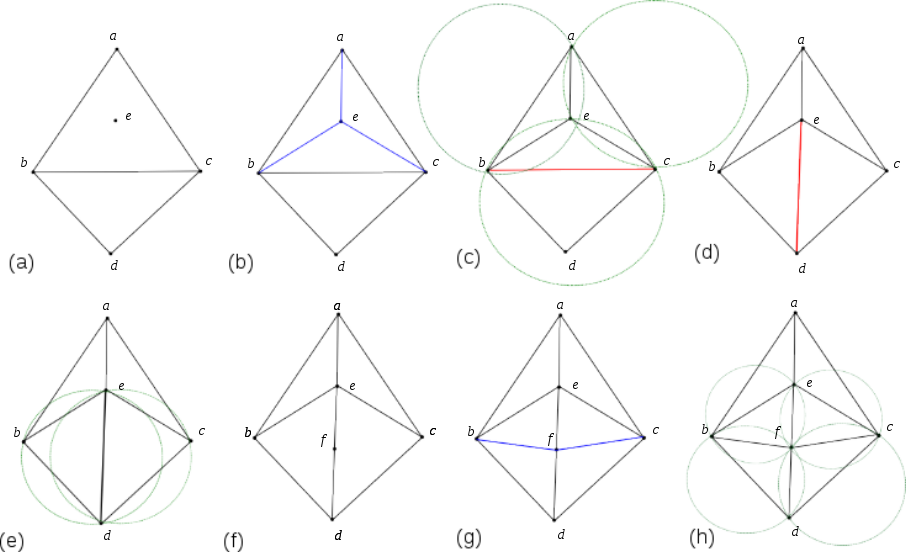
\includegraphics[width=350pt]{imagens_delaunay/green_sibson.png}
  \caption{\footnotesize{Aplicação do algoritmo de Green Sibson: (a) Tem-se a malha inicial com a inserção de um novo vértice que localiza-se dentro de um triângulo. (b) Divide-se o triângulo gerando três novos triângulos, formados pelas arestas em azul. (c) Realiza-se o teste dos circuncírculos e encontra-se uma aresta invadida, mostrada em vermelho. (d) Efetua-se o {\it flip} na aresta invadida. (e) Realiza-se o teste dos circuncírculos. (f) Ocorre a inserção de um novo vértice localizado sobre uma aresta. (g) Ocorre a divisão da aresta que contém o novo vértice, gerando quatro novos triângulos, compostos pelas novas arestas em azul. (h) Realiza-se o teste dos circuncírculos e verifica que não existe aresta invadida.
}}
  \label{fig_green_sibson}
\end{figure}

\begin{algorithm}[!ht]
\caption{Algoritmo de Green-Sibson.} 
\label{algoritmo_green_sibson}
\Entrada{Triangulação de Delaunay $TD$ e lista $L_V$ de vértices a serem inseridos em $TD$.}
\Saida{$TD$ com os vértices pertencentes à $L_V$.}
  \Inicio{
    \Para {(todo vértice $v \in L_V$)} {
	Inserir $v$ em $TD$; \\
	\eSe {($v$ localiza-se sobre aresta $\overline{ab} \in TD$)} {
	    Sejam $\Delta abc$ e $\Delta abd$ os triângulos que compartilham $\overline{ab}$; \\
	    Criar as arestas $\overline{av}$, $\overline{bv}$, $\overline{cv}$, $\overline{dv}$ e inserir em $TD$; \\
	}
	{
	    Seja $\Delta abc$ o triângulo que contém $v$; \\
	    Criar as arestas $\overline{av}$, $\overline{bv}$, $\overline{cv}$ e inserir em $TD$; \\
	}
    }
    \Para {(cada aresta $\overline{ab}$ criada)} {
	AlgoritmoLawson($\overline{ab}$);\\
    }
    \Retorna {$TD$;}
  }
\end{algorithm} 

\subsubsection {Refinamento de Delaunay} 
\label{cap_algoritmos_refinamento}
Nesta seção, são apresentados dois algoritmos no estado da arte para o refinamento de Delaunay: algoritmo de \citeonline{Ruppert1995} e \emph{off-centers} \cite{Ungor2004, Ungor2009, Oliveira2012a}.


\textbf {Algoritmo de Ruppert}
\label{cap_algoritmo_ruppert}

O algoritmo de \citeonline{Ruppert1995} garante que todos os triângulos pertencentes à triangulação terão ângulos entre $\alpha$ e $\pi-2\alpha$, de forma que $\alpha$ pode ser um ângulo máximo de aproximadamente 20,7 graus. Ao se inserir um vértice na triangulação, duas operações são possíveis: dividir um segmento e dividir um triângulo. Ao se dividir um segmento, um vértice é inserido em seu ponto médio. Ao se dividir um triângulo, um vértice é inserido em seu circuncentro. Com isso, uma nova triangulação é realizada \cite{Oliveira2012a}. 

Um algoritmo para a geração da triangulação de Delaunay pode utilizar uma medida de qualidade. Uma possível medida de qualidade chama-se \emph{Circunradius-to-shortest Edge Radio} (CER), que é definida pela razão do raio do circuncírculo \emph{r} (\emph{circunraio}) do triangulo, pela menor aresta \emph{l} do triângulo. É especificado um limite superior $\rho=r/l$ para o CER de todos os triângulos da malha. A razão $\rho$ de um triângulo está relacionada com seu menor ângulo ${\alpha}$ pela fórmula ${\rho = 1/[2\cdot sen(\alpha)]}$. Quanto menor for a razão $\rho$, maior será o ângulo $\alpha$ do triângulo. Esse limite superior $\rho$ garantirá que não há triângulo na malha com ângulo menor que ${\arcsin(1/2\rho)}$ \cite{Pebay2003}. 

Esse algoritmo pode receber como parâmetro de entrada um grafo planar de linhas não curvas (\emph {Planar Straight Line Graph} - PSLG). Um PSLG é um conjunto de vértices e seus segmentos. Segmentos são arestas que não podem ser removidos. Claramente, os segmentos não se interceptam. Um segmento é considerado invadido quando um vértice incide dentro de seu círculo diametral. Um pseudocódigo referente ao algoritmo de \citeonline{Ruppert1995} é apresentado no algoritmo (\ref{algoritmo_ruppert}).

\begin{algorithm}[!ht]
\caption{Refinamento de Ruppert.} 
\label{algoritmo_ruppert}
\Entrada{PSLG $G$.}
\Saida{Triangulação de Delaunay de $G$ com todos os $\measuredangle \geq \alpha$.}
\Inicio{
    Adicionar um delimitador quadrado $D$ à $G$: \\
    \Inicio{
      Calcular os extremos de $G$: $x_{min}$, $y_{min}$, $x_{max}$, $y_{max}$; \\
      Seja $span(G) = \max(x_{max} - x_{min}, y_{max} - y_{min})$; \\
      Seja $D$ o quadrado de lado $3 \times span(G)$, centralizado em $G$;\\
      Adicionar os quatro segmentos de contorno de $D$ à $G$; \\
    }
    Seja a lista de segmentos $L_{S} =$ arestas de $G$; \\
    Seja a lista de vértices $L_{V} =$ vértices de $G$; \\
    Construir a triangulação de Delaunay inicial $TD(L_{V})$;\\
    \Repita{ (at\'e que nenhum segmento esteja invadido e nenhum $\measuredangle < \alpha$) } 
    {
        \CommentSty{// Divide todos os segmentos invadidos em seu\\ // ponto m\'edio.}  \\  
	\Enqto{ (existe algum segmento $s \in L_{S}$ invadido) }
	{
	    $DividirSegmento(s)$; 
	}
	\CommentSty{ // Verifica tri\^angulos com $\measuredangle  < \alpha$.}  \\  
	\Enqto{ (existe algum tri\^angulo $\delta \in TD(L_{V})$ com $\measuredangle  < \alpha$;) }
	{
	    Seja $c$ o circuncentro de $\delta$; \\   	    
	    \eSe { ($c$ invade algum segmento $s \in L_{S}$) } 
	    {		
	        \CommentSty{// Divide todos os segmentos invadidos\\ // em seu ponto m\'edio.}  \\  
		$DividirSegmento(s)$; \\
	    }	    
	    {
	        \CommentSty{// Divide tri\^angulos com $\measuredangle < \alpha$, em seu\\ // circuncentro, adicionando $c$ \`a $L_{V}$.}  \\  
		$DividirTriangulo(\delta)$; \\
	    }   
	}
    }
    \Retorna {Triangulação de Delaunay corrente $TD(L_{V})$;}
}
\end{algorithm}  

Nas situações em que o PSLG possui ângulos menores que $90^{\circ}$, o algoritmo tende a formar triângulos com ângulos muito agudos. \citeonline{Shewchuk1997} provou que o algoritmo irá parar para qualquer entrada com ângulos de, no mínimo, $60^{\circ}$.

\textbf {\emph{Off-centers}}
\label{cap_off_centers}

\citeonline{Ungor2004,Ungor2009} propôs um refinamento de Delaunay similar ao algoritmo de \citeonline{Ruppert1995}. Em seu trabalho, introduz-se um novo tipo de pontos de {\it Steiner}, chamados {\it off-centers}, como uma alternativa aos circuncentros, apresentando um novo algoritmo de refinamento de Delaunay. Caso um triângulo seja considerado de má qualidade, pela medida CER, o algoritmo tenta inserir o \emph{off-center}. Caso o \emph{off-center} invada algum segmento, então, o novo vértice é inserido no ponto médio desse segmento em vez do \emph{off-center}. Um pseudocódigo referente a esse algoritmo pode ser observado no algoritmo (\ref{algoritmo_ungor}).

\begin{algorithm}[!ht]
\caption{Refinamento de \"Ungor.} 
\label{algoritmo_ungor}
\Entrada{PSLG $G$.}
\Saida{Triangulação de Delaunay de $G$ com todos os $\measuredangle \geq \alpha$.}
\Inicio{
    Seja $TD$ a triangulação de Delaunay dos vértices de $G$; \\
    Calcular: \\
    \ \ $B = $candidados à {\it off-centers} que invadem algum segmento;\\
    \ \ $C = $candidados à {\it off-centers} que não invadem segmentos;\\
    \ \ $D = $candidados à ponto médio;\\
    \Enqto{ ($C \cup D) \neq$ vazio }
    {
	Escolher um ponto $c_{o} \in (C \cup D)$ e inserir $c_{o}$ na triangulação $TD$; \\ 
	\Se { ($c_{o}$ é ponto médio de um segmento $s$)}
	{
	    $DividirSegmento(s)$;\\
	}
	Atualizar $TD$ e recalcular $B$, $C$ e $D$;
    }    
    \Retorna {Triangulação de Delaunay corrente $TD$;}    
}
\end{algorithm}  

Para calcular o {\it off-center}, considera-se um triângulo $\delta$, de má qualidade, formado pelos vértices $p$, $q$ e $r$. A menor aresta de $\delta$ é $pq$ e o seu circuncentro é $c$. O {\it off-center} $c_{o}$ de $\delta$ é o seu circuncentro se o CER do triângulo formado pelos vértices  $p$, $q$ e $c$ for menor ou igual a um dado limite $\rho_{\alpha}$, em que $\rho_{\alpha}$ é a medida CER de um ângulo $\alpha$, conforme mostrado na figura (\ref{fig_off_center}.a). Caso contrário, o {\it off-center} $c_{o}$ será o ponto na bissetora da aresta, dentro do circuncírculo, que faz com que o CER do triângulo $\Delta pqc_{o}$ seja exatamente igual a $\rho_{\alpha}$. A bissetora da aresta é a linha que passa pelo ponto médio de uma aresta de um triângulo e pelo seu circuncentro. 

O círculo que passa pelos vértices da menor aresta $pq$, centrado no {\it off-center}, é chamando {\it off-circle}. Caso o triângulo $\delta$ tivesse duas arestas menores iguais, escolheria-se uma delas, arbitrariamente. 

\begin{figure}[!ht]
  \centering
  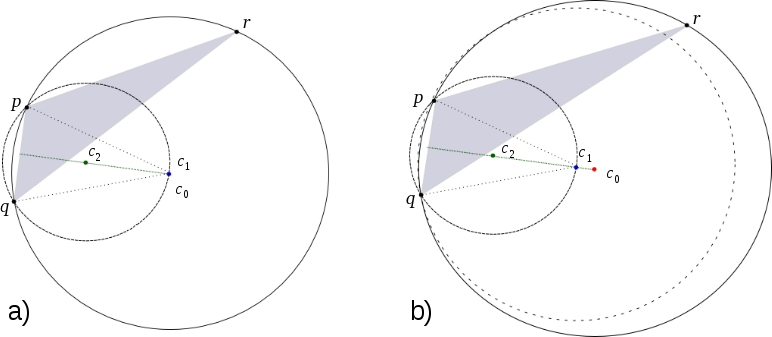
\includegraphics[width=300pt]{imagens_delaunay/off-center_A_B_rotulado.png}
  \caption{\footnotesize{ O {\it off-center} e o circuncentro do triângulo $\delta$, formado pelos vértices $p$, $q$ e $r$, são, respectivamente, $c_{0}$ e $c_{1}$. O circuncentro do triângulo formado pelos vértices $p$, $q$ e $c_{0}$ é $c_2$. Se $|c_{0} c_{2}| \leq \rho_{\alpha}|pq|$ então $c_{0} = c_{1}$, que é demonstrado em (a). Caso contrário, $c_{0} \neq c_{1}$. Nesse caso, calcula-se $c_{2}$ de forma que $|c_{0} c_{2}| = \rho_{\alpha}|pq|$, que é demonstrado em (b). O {\it off-circle} do triângulo $\delta$ é o circuncírculo em (a) e é mostrado em linhas tracejadas em (b). Figura adaptada de \citeonline{Ungor2004, Ungor2009}.
}}
  \label{fig_off_center}
\end{figure}

\citeonline{Ungor2004,Ungor2009} mostrou que seu algoritmo possui as mesmas garantias do algoritmo de Ruppert. Seus experimentos mostraram que seu algoritmo insere aproximadamente 40\% menos vértices que outros algoritmos de inserção no circuncentro e malhas 30\% menores em relação ao número de elementos.

\subsubsection{Resumo}

Nesta seção, apresentou-se a triangulação de Delaunay, um tipo de malha irregular que possui a propriedade de maximizar o menor ângulo da triangulação e o seu dual, o diagrama de Voronoi. 

Nas subseções (\ref{cap_algoritmo_lawson}), (\ref{cap_algoritmo_green_sibson}) e (\ref{cap_algoritmos_refinamento}) foram explanados um algoritmo para manutenção da triangulação de Delaunay, o algoritmo de \citeonline{Lawson1977}, um algoritmo para construção da triangulação de Delaunay, o algoritmo de \citeonline{Green1978}, e dois algoritmos para refinamento de Delaunay: o algoritmo de \citeonline{Ruppert1995} e \citeonline{Ungor2004,Ungor2009}.

\subsection{Discretização da equação do calor}
\label{cap_discretizacao_equacao_calor}

Nesta seção, aborda-se a discretização da equação do calor utilizando-se o método dos volumes finitos com o diagrama de Voronoi. Também mostra-se um pseudocódigo referente a esse método.

\subsubsection{Considerações iniciais}

No método dos volumes finitos (MVF), o domínio do problema é dividido em um conjunto finito de volumes, adjacentes entre si, chamados de volumes de controle (VC). Nesse método, realiza-se um balanço de conservação da propriedade em questão, para cada volume elementar, de modo a se obter a equação aproximada, respeitando-se a lei de conservação. Há interesse na aplicação do método dos volumes finitos na solução de equações diferenciais parciais (EDPs) devido a essa característica.

Uma forma de se obter as equações aproximadas no MVF é integrar, sobre cada volume elementar, no espaço e no tempo, as equações na forma conservativa, ou divergente. Nessa forma, os termos relacionados aos fluxos aparecem dentro das derivadas em relação às coordenadas espaciais. Ao realizar a integração para todos os VCs, obtém-se uma equação algébrica para cada volume e, consequentemente, obtém-se um sistema de equações algébricas. Esse sistema de equações é formado pelas variáveis localizadas nos centróides dos VCs. Para as aproximações, utilizam-se funções de interpolação por meio dos valores das variáveis dos VCs vizinhos. Devido a sua generalidade, qualquer tipo de malha pode ser utilizada, regular ou irregular \cite[p. 27 - 33]{Maliska2010}.

Na seção (\ref{cap_equacao_calor}), apresenta-se o modelo matemático para difusão de fluidos. Na seção (\ref{cap_discretizacao_malha_irregular}), é tratada a discretização da equação do calor com o diagrama de Voronoi e apresenta-se o pseudocódigo dessa discretização.

\subsubsection{Equação do calor}\label{cap_equacao_calor}

A equação do calor é um modelo matemático para a difusão de calor em sólidos, ou seja, descreve o fluxo de calor em um corpo sólido. Esse modelo consiste em uma equação de derivadas parciais que, muitas vezes, é também chamada de equação de difusão. Essa equação, em sua forma generalizada, é definida como

\begin{equation}
\frac {\partial } {\partial t} (\rho \phi)  =  \nabla \cdot \left( \frac {k} {c_{p}} \nabla \phi \right) ,
\label{equacao_diferencial_calor_forma_geral}
\end{equation}

\noindent em que $\phi$ é a temperatura, $t$ é o tempo, $\rho$ é a massa volumétrica do material, $c_{p}$ é o seu calor específico e $k$ é a condutibilidade térmica. 

Segundo \citeonline[p. 73]{Tannehill1997}, pode-se integrar a equação (\ref{equacao_diferencial_calor_forma_geral}) sobre um volume $V$ qualquer obtendo-se

\[
\iiint_V  \left ( \frac {\partial } {\partial t} (\rho \phi)  +  \nabla \cdot {\mathbf q} \right )dV = 0,
\]
\noindent com ${\mathbf q} =  - \frac {k} {c_{p}} \nabla \phi$. Aplicando-se o teorema de Gauss, tem-se

\[
 \iiint _{V}   \frac {\partial } {\partial t} (\rho \phi) dV  +   \oiint_{S} {\mathbf q} \cdot {\mathbf n}  dS = 0.
\]

O ``volume'' contém uma unidade de profundidade em problemas bidimensionais. Nesse caso, ${\mathbf n} dS$ pode ser representado por $i dy - j dx$ para um caminho de integração na fronteira em sentido horário. Essa equação segue a lei de conservação. O primeiro termo na equação, uma integral sobre o volume, significa a taxa de variação da energia armazenada no volume em função do tempo. O segundo termo é uma integral de linha sobre a superfície do volume e representa a vazão de energia ao longo da superfície do volume na unidade de tempo \cite[p. 72 - 76]{Tannehill1997}. 

\subsubsection {Discretização da equação do calor com o diagrama de Voronoi}\label{cap_discretizacao_malha_irregular}

Nesta seção, é tratada a  discretização da equação do calor (\ref{equacao_diferencial_calor_forma_geral}) com o diagrama de Voronoi. Uma partição do diagrama de Voronoi pode ser vista na figura (\ref{fig_malha_voronoi}), na página \pageref{fig_malha_voronoi}. Esta discretização baseia-se no capítulo 13 de \citeonline[p. 322 - 385]{Maliska2010} e no capítulo 8 de \citeonline[p. 243 - 266]{Versteeg2007}.

Na figura (\ref{fig_volume_controle_integracao}), mostra-se o volume elementar com centróide $P$, sobre o qual será realizada a integração, e o VC adjacente, com centróide $Nb_{i}$. A equação discretizada é obtida integrando-se a equação (\ref{equacao_diferencial_calor_forma_geral}) em cada VC, no intervalo de tempo de $t$ a $t+ \Delta t$. 

\begin{figure}[!ht]
  \centering
  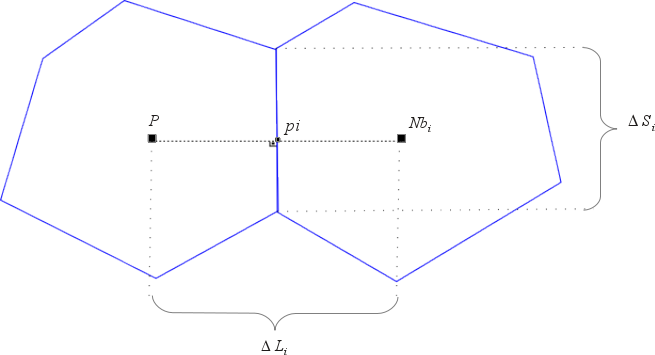
\includegraphics[width=200pt]{imagens_discretizacao/volume_controle_integracao.png}
  \caption{\footnotesize{Volumes de controle para a integração.
}}
  \label{fig_volume_controle_integracao}
\end{figure}

Integrando-se a equação (\ref{equacao_diferencial_calor_forma_geral}) no tempo e no espaço e adotando-se uma formulação implícita, obtém-se $
 \int_{t}^{t+ \Delta t}\int_{V} \frac {\partial} {\partial t} (\rho \phi) dV dt = \int_{t}^{t+ \Delta t} \int_{V} \nabla \cdot \left( \frac { k } { c_{p} } \nabla \phi \right) dV dt.$ O ponto de integração $pi$ localiza-se no ponto médio da interface dos polígonos com centróides $P$ e $Nb_{i}$. Aplicando-se o teorema da divergência e utilizando-se uma aproximação linear, tem-se

\begin{equation}
 \frac { M_{P}^{t + \Delta t} \phi_P^{t + \Delta t} - M_{P}^{t} \phi_{P}^{t} } { \Delta t} = \sum_{i=1}^{n} \left( \frac {k} {c_P} \left( \phi_{Nb_{i}}^{t + \Delta t} - \phi_{P}^{t + \Delta t} \right) \frac {\Delta S_{i}} {\Delta L_{i}} \right),
 \label {discretizacao_equacao_calor_1}
\end{equation}

\noindent em que $M_{P}=\rho \cdot A$ é a massa dentro do volume de controle e $A$ é a área do polígono com centróide $P$. $\phi_{P}$ é a temperatura do volume de controle com centróide $P$, $\phi_{Nb_{i}}$ é a temperatura no volume de controle com centróide $Nb_{i}$ e $n$ é o número de VCs adjacentes ao VC com centróide $P$. $\Delta S_i$ é o tamanho da interface entre os polígonos com centróide $P$ e seu polígono adjacente com centróide $Nb_i$ e $\Delta L_i$ é a distância entre os pontos $P$ e $Nb_i$. A equação (\ref{discretizacao_equacao_calor_1}) pode ser escrita como

\begin{equation}
 A_{P} \phi_{P}^{t+ \Delta t} - \sum_{i=1}^{n} A_{Nb_{i}} \phi_{Nb_{i}}^{t+ \Delta t} = B,
 \label{equacao_discretizacao_pologono_voronoi} 
\end{equation}

\noindent em que $A_{Nb_{i}} =  \frac{k} {c_{p}}  \cdot \frac {\Delta S_{i}} {\Delta L_{i}},  A_{P} = \sum_{i=1}^{n} A_{Nb_{i}} + \frac { M_{P}^{t+ \Delta t} } { \Delta t}$ e $B = \frac {M_{P}^{t} \phi_{P}^{t}} { \Delta t}.$

Caso um ou mais VCs adjacentes ao VC com centróide $P$ esteja localizado na fronteira e considerando-se condições de contorno de Dirichlet, a abordagem é da mesma forma que a empregada na seção anterior. Na aproximação linear da derivada na interface que separa o volume de controle com centróide $P$ e um volume de controle com centróide $F$, localizado na fronteira e adjacente ao VC com centróide $P$, terá o valor da temperatura de $F$ substituído pelo valor prescrito da condição de contorno. Os coeficientes $A_{Nb_{i}}$, $A_{P}$ e $B$ variam de acordo com a quantidade de VCs adjacentes localizados na fronteira. Com um centróide $F_{i}$ de um VC na fronteira, conforme pode ser visto na figura (\ref{fig_volume_controle_integracao_fronteira}), $\Delta S_{F_{i}}$ é o mesmo que $\Delta S_{i}$, ou seja, é o tamanho da interface entre os polígonos com centróide $P$ e seu polígono adjacente com centróide $F_i$ e $\Delta L_{F_{i}}$ é o mesmo que $\Delta L_{i}$, ou seja, é a distância entre os pontos $P$ e $F_i$. 

\begin{figure}[!ht]
  \centering
  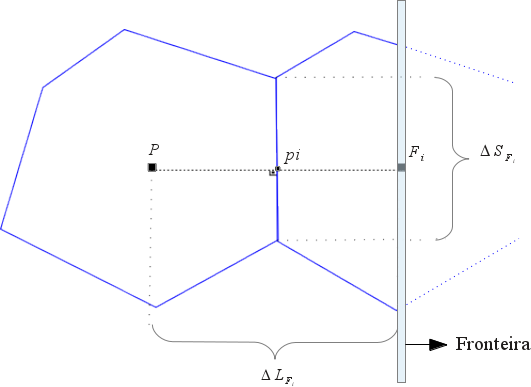
\includegraphics[width=180pt]{imagens_discretizacao/volume_controle_integracao_fronteira.png}
  \caption{\footnotesize{Volumes de controle para a integração com vizinho localizado na fronteira.
}}
  \label{fig_volume_controle_integracao_fronteira}
\end{figure}

A seguir, mostra-se um exemplo para ficar clara a forma com que se aplica o método dos volumes finitos com o diagrama de Voronoi nas ocorrências em que um VC contém VCs adjacentes na fronteira. Considere o volume de controle com  centróide $P_3$ mostrado na figura (\ref{fig_volume_voronoi_fronteira}). Os volumes adjacentes ao VC com centróide $P_3$, internos ao domínio, têm centróides $Nb_1$, $Nb_2$ e $Nb_3$ e os volumes  adjacentes ao VC com centróide $P_3$, localizados na fronteira, contêm valores prescritos e descritos nos pontos $F_1$, $F_2$ e $F_3$, $m_1$ é o número de volumes internos e adjacentes ao VC com centróide $P$, $m_2$ é o número de volumes de fronteira e adjacentes ao VC com centróide $P$ e $n = m_1 + m_2$.
Os valores das temperaturas nesses pontos são representados por $\phi_{F_{j}}$. Realizando-se a discretização da equação do calor para um volume localizado na fronteira, a equação (\ref{discretizacao_equacao_calor_1}) torna-se

\begin{figure}[!ht]
  \centering
  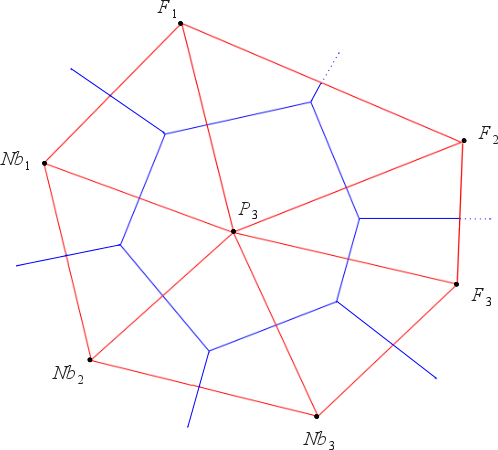
\includegraphics[width=150pt]{imagens_discretizacao/volume_voronoi_fronteira.png}
  \caption{\footnotesize{Volume de Voronoi adjacente a VCs com centróides localizados na fronteira. $Nb_1$, $Nb_2$ e $Nb_3$ são os centróides dos VCs internos ao domínio e $F_1$, $F_2$ e $F_3$ contêm valores prescritos em pontos localizados na fronteira.
}}
  \label{fig_volume_voronoi_fronteira}
\end{figure}


\begin{eqnarray}
 \frac { M_{P}^{t + \Delta t} \phi_P^{t + \Delta t} - M_{P}^{t} \phi_{P}^{t} } { \Delta t} &=& \sum_{i=1}^{m_1} \left( \frac {k} {c_P} \left( \phi_{Nb_{i}}^{t + \Delta t} - \phi_{P}^{t + \Delta t} \right) \frac {\Delta S_{i}} {\Delta L_{i}} \right) \nonumber \\
 & & + \sum_{i=1}^{m_2} \left( \frac {k} {c_P} \left( \phi_{F_{i}}^{t + \Delta t} - \phi_{P}^{t + \Delta t} \right) \frac {\Delta S_{F_{i}}} {\Delta L_{F_{i}}} \right), \nonumber
\end{eqnarray}

\noindent que pode ser reescrita como

\begin{equation}
 A_{P} \phi_{P}^{t+ \Delta t} - \sum_{i=1}^{m_1} A_{Nb_{i}} \phi_{Nb_{i}}^{t+ \Delta t}  = B,
 \label{equacao_discretizacao_pologono_voronoi_fronteira} 
\end{equation}

\noindent em que $A_{Nb_{i}} = \left( \frac{k} {c_{p}}  \frac {\Delta S_{i}} {\Delta L_{i}} \right), A_{F_{i}} = \left( \frac{k} {c_{p}}  \frac {\Delta S_{F_{i}}} {\Delta L_{F_{i}}} \right), A_{P} = \sum_{i=1}^{m_1} A_{Nb_{i}} + \sum_{i=1}^{m_2} A_{F_{i}} + \frac { M_{P}^{t+ \Delta t} } { \Delta t}, B = \frac {M_{P}^{t} \phi_{P}^{t}} { \Delta t} + \sum_{i=1}^{m_2} A_{F_{i}} \phi_{F_{i}}^{t+ \Delta t}$. Dessa forma, tem-se a discretização da equação do calor com polígonos de Voronoi.

A seguir, no algoritmo \ref{algoritmo_metodo_volumes_finitos}, é apresentado um pseudocódigo referente à discretização da equação do calor com polígonos de Voronoi, mostrado na figura (\ref{fig_malha_voronoi}). Um sistema de equações lineares é gerado, em que a equação de cada VC da malha, interno ao domínio ou localizado na fronteira é, respectivamente, conforme a equação (\ref{equacao_discretizacao_pologono_voronoi}) ou conforme a equação (\ref{equacao_discretizacao_pologono_voronoi_fronteira}).  No pseudocódigo, os valores dos coeficientes são armazenados em objetos que representam os vértices da triangulação de Delaunay. 

\begin{algorithm}
\caption{ Método dos volumes finitos.} 
\label{algoritmo_metodo_volumes_finitos}
\Entrada{lista dos v\'ertices da triangula\c{c}\~ao de Delaunay.}
\Saida{lista dos v\'ertices da triangula\c{c}\~ao de Delaunay com os coeficientes $A_{P}$, $A_{Nb_{i}}$ e $B$ preenchidos.}
\Inicio{
  \ParaCada{ ( v\'ertice interno P da triangula\c{c}\~ao de Delaunay) } 
  {
    \CommentSty{ // $Area_{P}$ é a \'area do VC com centr\'oide $P$}\\     
    $P.A_{P} \leftarrow \frac { \rho \cdot Area_{P} } { \Delta t};$  
    $P.B \leftarrow \frac { \rho \cdot Area_{P} } { \Delta t} \cdot P.valorTemperaturaEtapaAnterior;$\\
    \ParaCada{( v\'ertice $Nb_i$ adjacente a $P$)} {
      $P.A_{Nb_{i}} \leftarrow 0;$ \\ 
      \uSe { (v\'ertice $Nb_{i}$ localiza-se na fronteira)} {         
	\CommentSty{// $\Delta S_{F_{i}}$ e $\Delta L_{F_{i}}$ são calculados conforme\\ // mostrado na fig.(\ref{fig_volume_controle_integracao_fronteira})} \\           
	$P.A_{P} \leftarrow P.A_{P} +  \frac{k} {c_{p}}  \frac {\Delta S_{F_{i}}} { \Delta L_{F_{i}} };$ \\          
	\CommentSty{// $valorTemperatura$ \'e definida pelas\\ // condi\c{c}\~oes de contorno}\\     
	$P.B \leftarrow P.B + ( Nb_{i}.valorTemperatura \cdot \frac{k} {c_{p}}  \frac {\Delta S_{i}} { \Delta L_{i} });$ \\
	\CommentSty{// $Nb_{i}$ localiza-se na fronteira,\\ // portanto $F_{i} = Nb_{i}$  }\\           
      }\Senao {
	\CommentSty{// $\Delta S_{i}$ e $\Delta L_{i}$ são calculados conforme\\ // mostrado na fig. (\ref{fig_volume_controle_integracao})} \\           
	$P.A_{P} \leftarrow P.A_{P} +  \frac{k} {c_{p}}  \frac {\Delta S_{i}} { \Delta L_{i} };$ \\          
	$P.A_{Nb_{i}} \leftarrow P.A_{Nb_{i}} - \frac{k} {c_{p}} \frac {\Delta S_{i}} { \Delta L_{i} };$\\
      }
    }
  }
}
\end{algorithm}

\subsubsection{Resumo}

Nesta seção, abordou-se a discretização da equação do calor. Primeiramente, na subseção (\ref{cap_equacao_calor}), apresentou-se o modelo matemático que descreve a difusão de calor em sólidos. 
Na subseção (\ref{cap_discretizacao_malha_irregular}), utilizou-se o MVF com o diagrama de Voronoi. Por fim, apresentou-se um pseudocódigo referente a essa discretização.
 
\subsection{O método dos gradientes conjugados}
\label{cap_metodo_gradientes_conjugados}

Nesta seção, apresenta-se o método dos gradientes conjugados (MGC). Em seguida, definem-se os passos do MGC e elabora-se um pseudocódigo. Com o intuito de diminuir o número de iterações, explica-se como realizar o pré-condicionamento e o reordenamento dos vértices.  

\subsubsection{Considerações iniciais}

Um sistema linear, na forma de um produto matricial, pode ser visto como 

\begin{equation}
Ax = b,
\label{equacao_ax=b}
\end{equation}

\noindent de forma que ${A \in \mathbb{R}^{n \times n}}$ e os vetores $x , b \in \mathbb{R}^{n}$ são tomados como vetores coluna. A solução do sistema poderia ser calculada por meio da inversa da matriz $A$, considerando que $A$ seja inversível, na forma $x = A^{-1}b$. Porém, o cálculo da inversa apresenta imprecisão numérica, além de ser um algoritmo com complexidade $O(n^3)$. Ver \citeonline{Niedu2012}, para detalhes.

O MGC foi, inicialmente, proposto por \citeonline {Hestenes1952}. Foi, originalmente, desenvolvido como um método direto delineado para resolver um sistema linear $n \times n$ positivo definido  \cite [p.~479]{Burden2010}.

O MGC é útil na resolução de sistemas esparsos, de tamanho elevado, com $n$ na casa de milhares ou milhões, com entradas não nulas que aparecem em padrões predizíveis. Quando a matriz está pré-condicionada, de forma que os cálculos sejam eficazes, bons resultados são obtidos em, aproximadamente, $\sqrt{n}$ passos, tornando o MGC preferível em relação à eliminação gaussiana e a outros métodos iterativos  \cite[p.~479]{Burden2010}.

Na seção (\ref{cap_otimizacao}), mostra-se que, por meio da minimização de uma função, encontra-se a solução do sistema linear. Na seção (\ref{cap_construcao}), define-se o MGC e um algoritmo em pseudocódigo. Na seção (\ref{cap_pre_condicionamento}), mostra-se como realizar um pré-condicionamento.
Por fim, na seção (\ref{cap_conclusao}), tem-se o resumo deste capítulo.

\subsubsection{Otimização para resolução de sistemas lineares} \label{cap_otimizacao}

A solução de um sistema linear, conforme a equação (\ref{equacao_ax=b}), pode ser encontrada por meio da minimização de uma função $f(x) : \mathbb{R} \rightarrow \mathbb{R}$, sujeita a $x \in \mathbb{R}^n$. A demonstração de que a solução do sistema linear é encontrada a partir da minimização de $f(x)$ pode ser encontrada em \citeonline[p.~479]{Burden2010}. 

O vetor $x^*$ é uma solução do sistema linear definido positivo se e, somente se, $x^*$ minimiza

\begin{equation}
f(x)=\frac{x^TAx}{2} -b^Tx.
\label{equacao_f(x)}
\end{equation}

Ao derivar a equação (\ref{equacao_f(x)}) em relação ao vetor $x$, o resultado é um vetor também pertencente a $\mathbb{R}^n$, que satisfaz $\nabla {f(x^*)={Ax^*} -b = 0}$. O gráfico dessas funções apresenta um comportamento característico, de forma que o centro das curvas de nível é justamente o minimizador de $f(x)$.

\subsubsection{Definição do método} \label{cap_construcao}

O MGC consiste em, a partir de uma estimativa de solução inicial, minimizar o resíduo $r$, tal que $r = b - Ax$, a cada iteração $k$, em que $0 \leq k \leq n-1$, ao longo de direções conjugadas.  
Calcula-se a solução a partir de uma direção de busca $d_k$ e um coeficiente $\vartheta_k$, denominado comprimento do passo, conforme

\begin{equation} 
x_{k+1} = x_k + \vartheta_{k+1} d_{k+1}.
\label{equacao_xk}
\end{equation}

A direção de busca é definida de forma que

\begin{equation}
 d_k = r_{k-1} + \varphi_{k-1} d_{k-1} \\
\label{equacao_d_k}
\end{equation}

\noindent e o valor do resíduo $r_k$ é dado por

\begin{equation}
r_{k+1} = r_{k} - \vartheta_{k+1} A d_{k+1}.
\label{equacao_r_k}
\end{equation}

Os coeficientes $\vartheta_k$ e $\varphi_{k}$ são calculados conforme

\begin{equation}
  \vartheta_k =  \frac {r_{k-1}^T r_{k-1}} {d^{T}_k A d_k}
\label{equacao_alpha_4}
\end{equation}
e
\begin{eqnarray}
 \varphi_{k} = \frac{r_{k}^T r_{k}} {r_{k-1}^T r_{k-1}}.
\label{equacao_beta_k}
\end{eqnarray}

Dessa forma, o resíduo é minimizado ao longo das direções de busca. A estimativa inicial pode ser $x_0 = 0$, $r_0 = b$ e $d_1 = r_0$. O processo iterativo do MGC, formado pelas equações (\ref{equacao_xk}), (\ref{equacao_r_k}), (\ref{equacao_d_k}), (\ref{equacao_alpha_4}) e (\ref{equacao_beta_k}), pode ser descrito conforme apresentado no algoritmo (\ref{algoritmo_gradiente_conjugado}).

\begin{algorithm}
\caption{Método dos gradientes conjugados.}
\label{algoritmo_gradiente_conjugado}
\Entrada{Matrizes $A$ e $b$.}
\Saida{Solução $x$.}
$n \leftarrow \textrm {dimensão do vetor } x;$\\
\CommentSty{// Definir o erro admitido, por exemplo, $10^{-3}$.}\\
$\varepsilon \leftarrow 10^{-3};$ \\
\CommentSty{// O $erro$ deve ser maior que $\varepsilon$ na primeira iteração}\\
$erro \leftarrow \varepsilon + 1;$ \\
 \tcp{Valores para $i = 0$. $\vartheta_0$ e $\varphi_0$ não são necessários.}
$x_0 \leftarrow 0$\; 
$r_0 \leftarrow b - Ax_0$\;
$d_1 \leftarrow r_0$\;       
\tcp{Há $n+1$ termos ($0\leq i \leq n$)}
$i \leftarrow 1$\;
\Enqto{ $((i \leq n)$ e $(erro > \varepsilon))$} { 
 $ \vartheta_{i} \leftarrow \frac{r^T_{i-1} r_{i-1}}{d^T_{i} A d_{i}};$ \CommentSty{ // equação (\ref{equacao_alpha_4})} \\
 $ x_{i} \leftarrow x_{i-1} + \vartheta_{i} d_{i};$ \CommentSty{// equação (\ref{equacao_xk})}\\
 $erro \leftarrow \frac { || x_i - x_{i-1} ||_\infty } { ||x_i||_\infty};$ \CommentSty{ // $||x_i||_\infty$ é a norma infinita de $x_i$ } \\
 \tcp{Verifica se a próxima iteração será executada}
 \Se{$((i+1 \leq n)$ e $(erro > \varepsilon))$ }{
    $ r_{i} \leftarrow r_{i-1} - \vartheta_{i} A d_{i};$ \CommentSty{// equação (\ref{equacao_r_k})}\\ 
    $ \varphi_{i} \leftarrow \frac{r^T_{i} r_ {i}} {r^T_{i-1} r_{i-1}};$ \CommentSty{ // equação (\ref{equacao_beta_k})}\\
    $ d_{i+1} \leftarrow r_{i} + \varphi_{i} d_{i};$ \CommentSty{// equação (\ref{equacao_d_k})}\\
  }
 $i \leftarrow i + 1$\;
}
\end{algorithm}

\subsubsection{Pré-condicionamento} \label{cap_pre_condicionamento}

Segundo \citeonline[p.~486]{Burden2010}, ao utilizar um pré-condicionamento, o MGC não é aplicado diretamente na matriz A, mas sim em uma outra matriz positiva-definida. O pré-condicionamento consiste na substituição da equação (\ref{equacao_ax=b}) pelo sistema equivalente $C^{-1} Ax = C^{-1} b$, de forma que $C^{-1}$ seja escolhido com o objetivo de se melhorar o condicionamento do sistema original. Considerando-se $\tilde{A} = C^{-1} A (C^{-1})^T$, $\tilde{x} = C^{T} x$ e $\tilde{b} = C^{-1} b$, obtém-se a equação $\tilde{A} \tilde{x} = \tilde{b}$.

Dado que $ \tilde{r}_k = C^{-1}r_k$, $w_k = C^{-1} r_k$ e $\tilde{d}_k = C^{T}d_k$, as equações que geram o MGC podem ser reescritas, incorporando-se o pré-condicionamento. A equação (\ref{equacao_xk}), com o pré-condicionamento, fica

\begin{equation}
\tilde{x}_{k} = x_{k-1} +   \tilde{\vartheta} d_{k},
\label{equacao_xk_tilde}
\end{equation}

\noindent em que o parâmetro $\vartheta_k$, conforme a equação (\ref{equacao_alpha_4}), fica
\begin{equation}
\tilde{\vartheta}_{k} = \frac {w^{T}_{k-1} w_{k-1}} { d^{T}_{k} A d_{k}}.  
\label{equacao_alpha_til}
\end{equation}

A equação (\ref{equacao_r_k}) fica

\begin{eqnarray}
\tilde{r}_{k} = r_{k-1} - \tilde{\vartheta}_{k} A d_{k}.
\label{equacao_r_k_tilde}
\end{eqnarray}

A equação (\ref{equacao_d_k}) fica

\begin{eqnarray}
\tilde{d}_{k+1} = C^{-T} w_{k} + \tilde{\varphi}_{k} d_{k}.
\label{equacao_d_k_tilde}
\end{eqnarray} 

O parâmetro $\varphi_k$, conforme a equação (\ref{equacao_beta_k}), fica

\begin{equation}
\tilde{\varphi}_{k} = \frac{w^T_{k} w_{k}} {w^T_{k-1} w_{k-1}}. 
\label{equacao_beta_k_tilde}
\end{equation}

Com as equações (\ref{equacao_xk_tilde}), (\ref{equacao_alpha_til}), (\ref{equacao_r_k_tilde}), (\ref{equacao_d_k_tilde}) e (\ref{equacao_beta_k_tilde}), tem-se o MGC pré-condicionado.

\subsubsection{Cuthill-McKee reverso} 
\label{cap_cuthill_mckee_reverso}
Para se reduzir o custo de execução e armazenamento para se solucionar um problema pelo MGC é realizada a reordenação da matriz de coeficientes. Um algoritmo muito utilizado, por apresentar bons resultados, é o algoritmo de \citeonline{Cuthill1969}. \citeonline{George1971} verificou que a ordem inversa do reordenamento realizado pelo algoritmo de \citeonline{Cuthill1969} supera o original.

O algoritmo Cuthill-McKee reverso é um método de reordenação, que objetiva reduzir a largura de banda de uma matriz simétrica. A largura de banda de uma matriz é a maior distância do primeiro elemento não-nulo da matriz triangular inferior à diagonal principal. Segundo \citeonline{George1994}, dado que a largura de banda da $i$-ésima linha de uma matriz $A$, de dimensão $n$, é $\psi_i(A) = i - min\{ (1 \leq j \leq n) | a_{ij} \in A, a_{ij} \neq 0 \}$, a largura de banda $\psi$ da matriz $A$, é dada por 
\begin{eqnarray}
\psi(A) &=& \max \{\psi_i(A) |  1 \leq i \leq n \} \nonumber \\
        &=& \max \{ |i - j|, | a_{i,j} \in A, a_{i,j} \neq 0 \}. \nonumber
\end{eqnarray}
Esse algoritmo realiza o reordenamento dos vértices de modo que, na matriz gerada, os elementos não nulos irão localizar-se mais próximos da diagonal. Esse algoritmo não garante que será encontrada a menor largura de banda possível, no entanto, na prática, bons resultados são obtidos. 

Considera-se o {\it profile} $\zeta$, da matriz $A$, tal que $\zeta(A) = \sum_ {i=1}^{n} \psi_i(A)$, em que $n$ é o número de linhas da matriz $A$. \citeonline{George1971} verificou que o algoritmo Cuthill-McKee reverso apresenta resultados melhores em relação ao original, havendo, frequentemente, uma redução do {\it profile}, mas mantendo a largura de banda da matriz. 

No algoritmo (\ref{algoritmo_cuthill_mckee}), tem-se o pseudocódigo do algoritmo Cuthill-McKee reverso, baseado na busca em largura. Esse algoritmo difere-se do algoritmo de busca em largura convencional em relação à ordem de visitação dos vértices, que se dá em ordem crescente de grau dos vértices. A saída do algoritmo é a lista dos vértices ordenados.

\begin{algorithm}
\caption{Cuthill Mckee reverso}
\label{algoritmo_cuthill_mckee}
\Entrada{ Vértice raiz $r$}
\Saida{Lista $L$ de vértices ordenados}
\Inicio{
  $i \leftarrow 1;$ \\
  \CommentSty{// Insere v\'ertice raiz $r$ no final da fila.}  \\   
  $Fila \leftarrow r;$ \\
  \CommentSty{// Marca v\'ertice raiz $r$ como visitado.}  \\   
  $Visitou(r) \leftarrow Verdadeiro;$ \\
  \Enqto{ ($Vazia(Fila) = Falso $) } 
  {
    \CommentSty{// Remove o primeiro v\'ertice da fila.}  \\   
    $v \leftarrow Fila;$ \\
    \CommentSty{// Insere o v\'ertice $v$ na posi\c{c}\~ao $i$ da lista de\\ // v\'ertices ordenados.}  \\   
    $L(i) \leftarrow v;$ \\      
    $i \leftarrow i + 1;$ \\
    \CommentSty{// Ordena v\'ertices adjacentes \`a $v$ em ordem\\ // crescente de grau.}  \\   
    $OrdenaAdjacentes(v);$ \\
    \ParaCada{(vértice $w$ adjacente \`a $v$ em ordem crescente de grau)} 
    {
      \Se{ ($Visitou(w) = Falso$)} 
      {
	  \CommentSty{// Insere v\'ertice $w$ no final da fila.}  \\   
	  $Fila \leftarrow w$; \\
	  \CommentSty{// Insere o v\'ertice $w$ na posi\c{c}\~ao $i$ da\\ // lista de v\'ertices ordenados.}  \\   
	  $L(i) \leftarrow w;$ \\      
	  $i \leftarrow i + 1;$ \\	  
	  \CommentSty{// Marca v\'ertice $w$ como visitado.}  \\   
	  $Visitou(w) \leftarrow Verdadeiro;$ \\
      }
    }      
  }
  \CommentSty{// Inverte a ordem dos v\'ertices na lista $L$.} \\
  $InverterOrdem(L)$; \\
  \Retorna $L$; \\
}
\end{algorithm}  

\citeonline{Cuthill1969} verificaram que a qualidade da ordenação de seu algoritmo depende do vértice inicial. Uma opção proposta para vértice inicial é o vértice de grau mínimo, que apresenta bons resultados, embora sem garantias. Uma outra proposta é apresentada a seguir.

{\bf Vértice pseudoperiférico}

Um estudo, elaborado por \citeonline{George1979}, propõe utilizar um vértice inicial a partir de um par de vértices que se encontra o mais distante possível entre si. Alguns conceitos são importantes para entender o funcionamento desse algoritmo.

Considere um grafo $G = (L_V, L_E)$, em que $L_V$ é um conjunto de vértices e $L_E$ o conjunto de arestas do grafo $G$. A excentricidade de um vértice $v \in L_V$, é dada pela maior distância $d(v,u)$ entre $v$ e um vértice $u \in L_V$, tal que $u \neq v$, dado que a distância entre dois vértices é o tamanho do menor caminho entre eles. Um caminho é um conjunto ordenado de vértices distintos $(v_0,v_1,..., v_k)$, tal que $v_i$ é adjacente a $v_{i+1}$, ou seja $v_i \in adj(v_{i+1})$ para $i=0,1,...k-1$. Portanto, a excentricidade $\tau$ de $v \in L_V$ é dada pela maior distância, de forma que $\tau(v) = \max \{ (\forall u \in L_V \wedge u \neq v) d(v,u) \}$. O diâmetro $\kappa$ de $G$ é a maior excentricidade encontrada em $G$, ou seja, $\kappa(G) = \max \{ (\forall v \in L_V) \tau (v) \} = \max \{ (\forall v,u \in L_V) d(v,u) \}$. Um vértice periférico $v \in L_V$ é aquele cuja excentricidade é igual ao diâmetro do grafo, de forma que $\tau(v) = \kappa(G)$. Já um vértice pseudoperiférico possui sua excentricidade próxima ao diâmetro do grafo.

Uma  estrutura de nível de um dado nó $v \in L_V$ é o particionamento $\mathscr{L}(v)$ de $L_V$, satisfazendo $\mathscr{L}(v) = \{ L_{0}(v), L_{1}(v), ... L_{\tau(v)} (v) \}$ em que $L_{0} (v) = \{ v \}, L_{1} (v) = adj (L_{0} (v) )$ e $L_{i} (v) = adj( L_{i-1} (v) ) - L_{i-2} (v), i = 2, 3, ... \tau(v) $. Dessa forma, os vértices com excentricidade $\tau$ de $v$ se encontram no conjunto $L_{\tau(v)}(v)$. 

Com esses conceitos apresentados, é possível entender o funcionamento do algoritmo (\ref{algoritmo_pseudo_periferico}), que apresenta um pseudocódigo referente ao algoritmo de \citeonline{George1979}.

\begin{algorithm}
\caption{Encontrar v\'ertice pseudoperif\'erico}
\label{algoritmo_pseudo_periferico}
\Entrada{ Vértice raiz $v$}
\Saida{ V\'ertice pseudoperif\'erico $t$}
\Inicio{
  \CommentSty{// Construir a estrutura de n\'ivel de $v$.}  \\   
  $\mathscr{L}(v) = \{  L_{0}(v), L_{1}(v), ..., L_{\tau(v)} (v) \};$ \\
  \Repita{ ( $u = v$ ) } 
  {
    \CommentSty{// $u$ \'e utilizado como controle do la\c{c}o de \\ // repeti\c{c}\~ao.}  \\   
    $u \leftarrow v;$ \\
    \CommentSty{// Busca entre os v\'ertices de maior\\ // excentricidade aquele com grau m\'inimo.}  \\   
    $t \leftarrow$ V\'ertice com grau m\'inimo $\in L_{\tau(v)} (v);$ \\  
    \CommentSty{// Construir a estrutura de n\'ivel de $t$.}  \\   
    $\mathscr{L}(t) = \{  L_{0}(t), L_{1}(t), ..., L_{\tau(t)} (t) \};$ \\    
    \CommentSty{// Verifica qual tem maior excentricidade.}  \\   
    \Se{($\tau(t) > \tau(v)$)} 
    {   
	$v \leftarrow t;$ \\
    }    
  }
  $t \leftarrow v;$ \\
  \Retorna $t$;
}
\end{algorithm}  

\subsubsection{Resumo} \label{cap_conclusao}

Nesta seção, apresentou-se a defininção do MGC bem como as suas principais características. Também foi descrito um pseudocódigo, que pode ser observado no algoritmo (\ref{algoritmo_gradiente_conjugado}), página \pageref{algoritmo_gradiente_conjugado}, a fim de resolver um sistema linear do tipo $Ax = b$. 

Com o intuito de se otimizar o número de iterações, na subseção (\ref{cap_pre_condicionamento}), foi apresentado como realizar o pré-condicionamento da matriz de coeficientes. Também foi exposto, na subseção (\ref{cap_cuthill_mckee_reverso}), um algoritmo de reordenação da matriz de coeficientes, o algoritmo Cuthill-McKee reverso, conforme o algoritmo (\ref{algoritmo_cuthill_mckee}), na página \pageref{algoritmo_cuthill_mckee}. Ainda, a fim de melhorar o desempenho do algoritmo de reordenação, apresentou-se um algoritmo que busca um vértice pseudoperiférico, utilizado como vértice inicial no algoritmo de reordenação, que pode ser observado no algoritmo (\ref{algoritmo_pseudo_periferico}), página \pageref{algoritmo_pseudo_periferico}.

 
\subsection{Suavização laplaciana}
\label{cap_suavizacao_laplaciana}

Uma forma de melhorar a qualidade da malha é aplicar um método de suavização, que reduz a distorção dos elementos ajustando a localização dos nós. Um método de suavização bastante conhecido é a suavização laplaciana, que move um vértice para o baricentro do polígono formado pelos seus vértices incidentes. Segundo \citeonline{Freitag1997}, esse método opera heuristicamente e não garante a melhoria na qualidade dos elementos. A forma simplificada da suavização laplaciana, aplicada a um nó $P$, pode ser escrita na forma 
\[
S_{P}^{n+1} = S_{P}^{n} + \beta \frac{ \sum_{i=1}^{m} \omega_{P,i}(S_{i}^{n} - S_{P}^{n}) } { \sum_{i=1}^{m} \omega_{P,i} }, 
\]
\noindent em que $S_{P} = (x,y)$ é a posição do vértice $P$ para duas dimensões, $S_{P}^{n+1}$ é a posição do nó $P$ na etapa $n+1$ de suavização, $S_{i}$'s são as posições dos nós adjacentes a $P$, $\omega_{P,i}$ é o peso da aresta que conecta $P$ ao $i$-ésimo nó vizinho e $ 0 < \beta < 1$ é um parâmetro de adaptatividade que controla a amplitude do movimento, definido localmente ou globalmente. 

Com o intuito de evitar as possíveis distorções de sucessivas iterações, \citeonline[seção 3]{Taubin1995} e \citeonline[seção 2]{Taubin1995A} propôs combinar duas suavizações sucessivas: $S_{P}^{n+1} = S_{P}^{n} + \lambda \Delta S_{P}^{n}$ e $S_{P}^{n+2} = S_{P}^{n+1} - \mu \Delta S_{P}^{n+1}$, em que $\Delta S_{P}^{n} =  \frac{ \sum_{i=1}^{m} \omega_{P,i}(S_{i}^{n} - S_{P}^{n}) } { \sum_{i=1}^{m} \omega_{P,i} }$ e os parâmetros quantificadores do movimento $0 < \lambda < \mu$. \citeonline{Taubin1996} ainda analisam as propriedades desse método e expõem como minimizar seu tempo de execução. Essa suavização é também chamada de suavização $\lambda/\mu$. \citeonline{Kobbelt1998} orientou utilizar $\lambda = \mu = 1$, nomeando esse método de suavização bi-laplaciana.
 
\subsection{Malhas móveis}
\label{cap_malhas_moveis}
Nesta seção, aborda-se alguns detalhes sobre malhas móveis, como o princípio de equidistribuição e a computação em malhas móveis. Também são apresentados trabalhos que pretendem solucionar equações diferenciais parciais por diferentes métodos, como o método dos volumes finitos, dos elementos finitos e das diferenças finitas, utilizando os mais variados tipos de malhas, como, por exemplo, o diagrama de Voronoi. Também são apresentadas técnicas de movimento de vértices baseadas em formulação laplaciana e trabalhos que utilizam a suavização laplaciana para melhorar a qualidade da malha.

\subsubsection{Considerações iniciais}

A utilização de métodos adaptativos de malhas proporciona uma melhora significativa na precisão e eficiência na geração de malhas. Os métodos de malhas móveis possuem vantagem em relação ao refinamento adaptativo por inserção de nós pois, com o aumento da quantidade de nós há o aumento do esforço computacional necessário para solucionar a malha. Os métodos em que ocorrem inserção de nós são robustos em problemas com regiões de rápida variação de acordo com o tempo mas, tendem a se tornar ineficientes devido ao contínuo reajuste, tornando sua execução dispendiosa \cite[p. 709]{Huang1994A}. 

Muitas pesquisas são focadas em obter soluções com baixo esforço computacional e alta precisão na aproximação, utilizando malhas adaptativas para simular fenômenos físicos. Algumas dessas pesquisas utilizam malhas móveis com discretizações de EDPs por volumes finitos (por exemplo, \citeonline{Mackenzie1996}, \citeonline{Van2006}, \citeonline{Tan2004}, \citeonline{Tan2006}, \citeonline{Springel2009,Springel2011}). Mesmo com os recentes avanços obtidos nessas e em outras pesquisas, acredita-se que pode-se obter um esquema de malhas móveis mais simples que os apresentados na literatura, com custo computacional bastante baixo.

Na próxima seção, (\ref{cap_adaptatividade}), aborda-se uma classificação dos métodos adaptativos para resolução de equações diferenciais parciais. Explica-se o princípio de equidistribuição na seção (\ref{cap_principio_equidistribuicao}) e, na seção (\ref{cap_computacao_malhas_moveis}), a computação em malhas móveis. Apresenta-se, na seção (\ref{cap_revisao_metodos_malhas_moveis}), uma revisão dos métodos de malhas móveis na resolução de diversos problemas. Na seção (\ref{cap_movimento_laplaciano}), apresentam-se trabalhos que realizam melhorias na qualidade da malha por meio da suavização laplaciana e, na seção (\ref{trabalhos_laplacianos}), tem-se trabalhos que realizam o movimento dos vértices baseado na formulação laplaciana, com o intuito de obter melhorias na aproximação da solução da EDP. Por fim, na seção (\ref{cap_malhas_moveis_consideracoes_finais}), tem-se o resumo desta seção.

\subsubsection{Adaptatividade}
\label{cap_adaptatividade}

É comum impor alguma forma espacial na malha e, em seguida, discretizar a solução, utilizando-se elementos finitos, diferenças finitas ou volumes finitos. No entanto, tal estratégia pode não ser eficaz no caso de estruturas que envolvam escalas de pequeno comprimento, ocasionando grandes erros. Nesses casos, pode ser benéfico utilizar alguma forma não uniforme de malha, adaptada para a solução, na qual serão realizados os cálculos. As vantagens dessa estratégia podem ser a redução dos erros, melhor condicionamento do sistema e melhor eficiência computacional. Infelizmente, isso adiciona um nível extra de complexidade ao sistema, que pode conduzir a um custo computacional adicional e também a uma possível instabilidade numérica \cite{Huang2009}.

Métodos adaptativos para resolução de equações diferenciais parciais podem ser divididos em três categorias: abordagem {\it h} de refinamento, abordagem {\it p} de refinamento e abordagem {\it r} de refinamento. Segundo \citeonline{Oliveira2013}: 

\begin{quotation}
Na abordagem {\it h}  de refinamento, inicia-se a simulação com uma malha inicial e essa malha é refinada ou simplificada por meio da inclusão ou da remoção de pontos. Geralmente, a estratégia utilizada na inclusão ou na remoção dos pontos é orientada por uma estimativa a {\it posteriori} de erro da solução. Isso é chamado, geralmente, de refinamento adaptativo de malhas por usuários do método dos volumes finitos.  

Na abordagem {\it p} de refinamento, segundo \apudonline{Huang2009}{Oliveira2013}, utiliza-se uma discretização de EDPs por elementos finitos com polinômios de uma ordem particular. Essa ordem é incrementada ou decrementada de acordo com os erros da solução. Pode-se combinar essa abordagem com o refinamento {\it h} para se utilizar uma estimativa a {\it posteriori} de erro da solução. Com essa combinação, tem-se a subcategoria de refinamento {\it hp}, cujo objetivo é a obtenção da solução dentro de um erro prescrito limitado pelos procedimentos de refinamento \apud{Huang2009}{Oliveira2013}.

No refinamento {\it r}, o número de pontos da malha é fixo e esses pontos são movidos de forma que sejam concentrados nas regiões de grande variação da solução em função do tempo. Na comunidade de volumes finitos, são chamados, geralmente, de malhas móveis.  Segundo \apudonline{Eleftheriou2011}{Oliveira2013}, essa abordagem de refinamento pode ser, em geral, utilizada para  problemas transientes por causa da mobilidade da malha, que  facilita lidar com integradores de tempo. Entretanto, sua limitação está na dificuldade em definir um intervalo de tempo adequado, uma vez que os nós variam de posição ao longo do tempo, podendo ocorrer o entrelaçamento de arestas. Ainda, a aplicabilidade da adaptatividade {\it r} é limitada devido ao número fixo de graus de liberdade e a uma conectividade constante dos  polígonos da malha. Com isso, a adaptatividade {\it r} é, tipicamente, utilizada para acelerar o processo computacional em vez de ser utilizada para se alcançar uma precisão prescrita. 
\end{quotation}

No contexto de malhas móveis, a análise da adaptatividade foca em como otimizar a escolha dos pontos da malha, de forma que o custo computacional seja correlacionado com o número de pontos utilizados \cite{Huang2011}. Os pontos da malha são concentrados em regiões em que há erro ou gradiente grande da solução. Segundo \citeonline{Huang2011}, a análise da adaptatividade foca em como otimizar a escolha dos pontos da malha, de forma que o custo computacional é correlacionado com o número de pontos utilizados na malha. A adaptatividade {\it r} deriva do princípio de realocação, pois a localização dos pontos é dinamicamente realocada durante o curso da computação numérica \cite{Huang2011}.

Segundo \citeonline{Oliveira2013}: 

\begin{quotation}
Como afirmam \apudonline{Huang2011}{Oliveira2013}, os métodos de malhas móveis ainda estão em uma fase relativamente inicial de desenvolvimento. Muitos deles estão em estágio experimental e, quase todos, requerem uma justificativa matemática adicional. Como também explicam \apudonline{Huang2011}{Oliveira2013}, uma análise rigorosa dos métodos de malhas móveis, para resolver EDPs dependentes do tempo, só foi realizada para alguns modelos muito simples de problemas. Ainda, também explicam que muitas formas de se melhorar sua eficiência e robustez serão, sem dúvida, desenvolvidas. Como, por exemplo, ainda são necessários mais estudos numéricos sistemáticos de como se reduzir os custos na resolução de todo um sistema de malha e EDPs, bem como estudos em como equilibrar a adaptação espacial e temporal de uma malha.
\end{quotation}

\subsubsection{Princípio da equidistribuição}
\label{cap_principio_equidistribuicao}

Segundo \citeonline{Oliveira2013}:
\begin{quotation}
O princípio de equidistribuição (PE) foi originalmente introduzido por \apudonline{Boor1973}{Oliveira2013}. Com esse princípio, busca-se rearranjar os nós de uma malha de forma que uma determinada medida seja distribuída equitativamente ao longo de cada subintervalo da malha. Essa medida pode ser, por exemplo, uma medida de erro que será comparada com a medida de um elemento
desejável, hipoteticamente ótimo. A diferença entre cada elemento da malha e o elemento desejável será, aproximadamente, a mesma para todos os elementos existentes. De acordo com \apudonline{Askes2000}{Oliveira2013}, algumas restrições topológicas, como cantos não convexos em problemas multidimensionais, podem impedir um movimento de pontos ideal, por isso, não se pode garantir que a equidistribuição seja satisfeita para todos os elementos da malha. 
\end{quotation}

Segundo \citeonline{Oliveira2013}, ao aplicar o PE em um problema unidimensional, redefine-se a posição dos nós, distribuindo-se, equitativamente, um medida denominada função peso, em todo o domínio. Em um problema unidimensional, por exemplo, a posição dos nós $x_i$, para $i= 1..N$ é realocada, distribuindo-se a função peso $M(x)$ em todo o domínio, conforme $\int_{x_{i-1}}^{x_i} M(x)dx = \int_{x_i}^{x_{i+1}} M(x)dx$, para $1 \leq i \leq N-1$.  No formato discreto, essa equação é aproximada por
\begin{equation}
 M_{i-1} \Delta x_{i-1} = M_i \Delta x_i, \textrm{ para } 1 \leq i \leq N-1,
 \label{funcao_monitora_auxiliar_um}
\end{equation}

\noindent em que $\Delta x_{i-1} = x_i - x_{i-1}$ é o tamanho local da malha e $M_{i-1}$ representa a estimativa discreta de $M(x)$ no intervalo $[x_{i-1}, x_i]$. Com a distribuição uniforme ao longo de todo o domínio, tem-se que $\frac{1}{N}\int_{x_0}^{x_N} M(x)dx = \int_{x_i}^{x_{i+1}} M(x)dx = c$, para $0 \leq i \leq N-1$, em que $c$ é uma constante.

Segundo \citeonline{Oliveira2013}, as primeiras aplicações do PE, os trabalhos de \citeonline{Dwyer1979}, \citeonline{Dwyer1981}, \citeonline{Gnoffo1980} e \citeonline{White1982} resolvem problemas em mecânica dos fluidos e transferência de calor em uma dimensão. \apudonline{White1982}{Oliveira2013} recorreu ao comprimento do arco da solução como função monitora,

\begin{equation}
 M(u) = \sqrt{1+ | u' | ^2} .
 \label{funcao_monitora_auxiliar_dois}
\end{equation}

Considere-se um exemplo unidimensional, retirado de \citeonline{Oliveira2013} o qual foi originalmente adaptado de \citeonline{Tan2005}, para ilustrar a ideia principal do PE. Seja $f(x) = tanh \left( \frac{1-x}{0.1} \right)$. Considere-se ainda um subconjunto no intervalo $[0,1]$. Suponha-se agora que $x_0 < x_1 < ... < x_n$, em que $x_0 = 0$ e $x_n = 1$. Neste contexto, no gráfico à esquerda da figura (\ref{fig_principio_equidistribuicao}), a malha é dividida uniformemente, podendo-se observar a malha adaptativa gerada pelo PE no gráfico à direita da figura (\ref{fig_principio_equidistribuicao}). Nesse caso, a função monitora foi baseada no comprimento do arco, expressa por (\ref{funcao_monitora_auxiliar_dois}) e os pontos são distribuídos igualmente na curva da solução satisfazendo (\ref{funcao_monitora_auxiliar_um}). 

\begin{figure}[!ht]
  \centering
  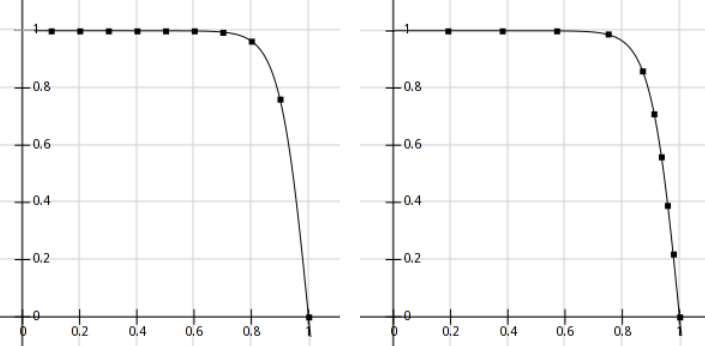
\includegraphics[width=200pt]{imagens_malhas_moveis/principio_equidistribuicao.png}
  \caption{\footnotesize{Comparação entre o PE utilizando o comprimento do arco (à direita) e uma malha dividida uniformemente (à esquerda) com dez pontos. Exemplo extraído de \citeonline{Oliveira2013} e originalmente adaptado de \citeonline{Tan2005}.
}}
  \label{fig_principio_equidistribuicao}
\end{figure}

Exemplos similares podem ser encontrados em \citeonline{Zegeling1996}, \citeonline{Li2000} e \citeonline{Tan2005}. Para mais informações sobre o PE, verifique \citeonline{Huang2011}, onde se apresentam os princípios básicos da adaptatividade e estratégias de movimentos de malha em casos unidimensionais e multimensionais.

\subsubsection{Computação em malhas móveis}
\label{cap_computacao_malhas_moveis}

\begin{quotation}

Segundo \apudonline{Huang2011}{Oliveira2013}, o problema de se computar soluções de EDPs, utilizando métodos de malhas móveis pode ser separado em três problemas:
\begin{itemize}

\item Uma função de densidade da malha, também chamada de função monitora, é necessária para guiar a redistribuição dos pontos da malha na evolução da EDP. Essa função monitora, normalmente, é restrita tanto para equidistribuir essa redistribuição, quanto para se obter um relaxamento da malha na busca de um estado equidistribuído. A escolha da função monitora pode depender do comprimento de arco da solução em problemas unidimensionais, na curvatura da solução e em erros {\it a posteriori} \apud{Huang2011}{Oliveira2013}. 

\item Determinada a função monitora, deve-se verificar uma malha que se equidistribui de alguma maneira. O problema da equidistribuição em si é um problema algébrico não linear \apud{Huang2011}{Oliveira2013}. 

\item A EDP é, então, discretizada, tanto no domínio computacional da malha quanto no domínio físico original e, geralmente, elementos finitos ou volumes finitos são empregados \cite{Oliveira2013}.
\end{itemize}

Na prática, qualquer que seja a escolha da função monitora, alguma suavização espacial (e temporal) é empregada. Segundo \apudonline{Huang2011}{Oliveira2013}, a chave para o sucesso dos métodos de malhas móveis reside na escolha adequada dessa função de densidade da malha. Essa função controla a concentração de pontos na malha por meio do PE e, tipicamente, mensura-se a dificuldade na aproximação numérica espacial do problema fundamental. Ainda de acordo com \apudonline{Huang2011}{Oliveira2013}, a seleção da função de densidade da malha pode ser baseada na estimativa de erro de interpolação, na invariância de escala ou em uma estimativa de erro {\it a posteriori}, com o limite ótimo para o erro de interpolação ou o erro da solução, também obtido pela malha equidistribuída correspondente \cite{Oliveira2013}. 
\end{quotation}

\citeonline{Huang2011} apresentam diversas equações de malhas para problemas estacionários e dependentes do tempo, abordando-se questões práticas de implementação, incluindo a discretização de equações de malhas e questões sobre adaptatividade de malhas no contexto multidimensional.

\subsubsection{Uma revisão de métodos de malhas móveis}
\label{cap_revisao_metodos_malhas_moveis}

Já foi desenvolvida e aplicada uma grande variedade de métodos de malhas móveis, de uma e duas dimensões, na resolução de diversos problemas, conforme pode-se verificar, por exemplo, em \citeonline{Hawken1991} e \citeonline{Tang2005}, em que há revisão de técnicas em malhas móveis de suas aplicações na dinâmica de fluidos computacional. Ainda, vários outros métodos, especialmente multi-dimensionais, têm sido desenvolvidos e utilizados com sucesso \cite{Tan2004, Tan2006, Springel2009, Springel2011}.

A seguir, são apresentadas algumas propostas de resolução de problemas utilizando malhas móveis. Também são apresentados alguns dos trabalhos desenvolvidos por Tan e seus colaboradores e por Springel e outros colaboradores. 

\textbf{Algumas propostas de malhas móveis}
\label{subcap_algumas_propostas_malhas_moveis}

De acordo com \citeonline{Marlow2010}, os métodos para movimentar os pontos de uma malha podem ser classificados em duas formas: os métodos com base na localização dos pontos e os métodos com base na velocidade dos pontos. Nos métodos com base na localização, utiliza-se um método para controlar diretamente a posição dos pontos da malha e, nos métodos com base na velocidade, um método é utilizado apenas para proporcionar a velocidade da malha, encontrando-se a posição dos pontos por um esquema a cada intervalo de tempo, como o método {\it Forward} Euler. Dois trabalhos apresentam uma visão geral desses métodos: \citeonline{Hawken1991}, comentado anteriormente nesta seção, e \citeonline{Huang2009}. Em \citeonline{Marlow2010, Marlow2011}, utilizam-se malhas móveis com elementos finitos contínuos para resolver EDPs parabólicas não lineares com fronteiras móveis por meio de um método adaptativo. \citeonline{Marlow2010, Marlow2011} descrevem os métodos utilizados em detalhes. Também são apresentados exemplos computacionais, com diferentes funções monitoras aplicadas à equação de meios porosos, em uma e duas dimensões espaciais.

\citeonline{Duffell2011} generalizam o método para a solução numérica de sistemas de equações hiperbólicas utilizando um diagrama de Voronoi dinâmico. O diagrama de Voronoi foi utilizado para gerar malhas móveis para a solução de sistemas multidimensionais das leis de conservação na forma de volumes finitos. Os pontos da malha são livres para se movimentar com uma velocidade arbitrária, de modo que a escolha da velocidade zero resulta na formulação euleriana. Movimentar os pontos na velocidade local do fluido torna a formulação efetivamente lagrangeana. Um código, TESS, foi escrito para resolver as equações hidrodinâmicas e magneto-hidrodinâmicas compressíveis para fluidos relativistas e não relativistas. Esse código foi modularizado, tornando-o facilmente adaptado para solucionar sistemas de equações gerais.

\citeonline{Olivier2011} realizaram simulações, em 3D, envolvendo geometrias móveis sujeitas, potencialmente, a grandes deslocamentos. Apresentaram dois métodos para lidar com deslocamentos grandes nas simulações com malhas móveis: o primeiro método consiste em movimentar a malha, o quanto for possível, mantendo a topologia fixa. Um inconveniente é que, ao movimentar a malha com uma topologia fixa, piora-se a forma dos elementos, o que influencia negativamente na precisão da solução e também retarda a computação, pois o intervalo de tempo é controlado pelo elemento mínimo de malha, isto é, a abordagem é sujeita à condição Courant-Friedrichs-Lewy (CFL) \cite{Courant1928}. O segundo método objetiva manter a qualidade da malha o melhor possível, enquanto movimenta os pontos, refazendo a malha utilizando 
operações locais, como adição de vértices, colapsos de vértices, alterações na conectividade e deslocamento dos vértices. Essa estratégia permite manter a qualidade da malha aceitável, entretanto, isso induz a um número grande de etapas de interpolação. Detalhes desse método podem ser encontrados em \citeonline{Lohner1999, Bruchon2009, Frey2008, Compere2010}. Um solucionador HLLC ({\it Harten-Lax-van Leer-Contact}) \cite{Toro1994} aproximado de Riemann é utilizado em \citeonline{Olivier2011}. Também utiliza-se um método de reconstrução do tipo MUSCL para melhorar a precisão do sistema. 

\citeonline{Mcnally2012} utilizam uma metodologia rigorosa para comparar resultados de diferentes códigos em duas dimensões para a solução do problema de instabilidade de Kelvin-Helmholtz (KHI). O KHI é uma das mais importantes instabilidades hidrodinâmicas e representa uma regra signifitiva em várias partes da astrofísica. O problema é testado nos códigos Pencil Code \footnote{http://pencil-code.nordita.org/}, Athena \footnote{https://trac.princeton.edu/Athena/}, Enzo \footnote{http://enzo-project.org/}, NDSPMHD \footnote{http://users.monash.edu.au/\~{ }dprice/software/index.html} e no código Phurbas \cite{Maron2012}.

\citeonline{Silva2012} propuseram uma técnica alternativa para atualização de malhas que se submetem a alterações geométricas e topológicas. Explora-se a propriedade {\it Weighted Delaunay Triangulation}, que pode ser utilizada para, implicitamente, definir a conectividade da malha. Em vez de se manterem as informações de conectividade, simplesmente, mantém-se uma coleção de pesos associados a cada vértice. Essa propriedade da triangulação de Delaunay é o fato de que todos os vértices podem ser emergidos em um poliedro convexo em uma dimensão extra, também conhecida como {\it lifting property}. Porém, o mesmo não se aplica a malhas que não são de Delaunay. Nesse trabalho também descreve-se um mecanismo para suavização das transições entre as malhas emergidas com diferentes níveis de refinamento. %Em síntese, as principais características desse trabalho são:

\textbf{Proposta de Tan e colaboradores e trabalhos relacionados}
\label{subcap_proposta_tan_colaboradores}

\citeonline{Tan2004} mostraram que, nos métodos de malhas móveis, os intervalos de tempo são proporcionais ao tamanho do menor volume espacial da malha e, como resultado, os volumes são cada vez menores a cada intervalo de tempo. Nesse trabalho, foi desenvolvido um algoritmo de escalonamento local de tempo para métodos de malhas móveis. A ideia principal foi apresentada pela investigação das leis de conservação não lineares hiperbólicas. 

\citeonline{Tan2006} propuseram um método simples de malha móvel para resolver equações de campo de fases. Sua estratégia numérica baseou-se na abordagem proposta em \citeonline{Li2000} para separar a malha móvel e a evolução da EDP. As equações de campo de fases foram discretizadas por um método dos volumes finitos e o movimento da malha foi realizado resolvendo as equações euleriana-lagrangeanas com a função monitora baseada em gradiente.

\citeonline{Tan2007} resolveu problemas magneto-hidrodinâmicos (MHD) por meio de técnicas de malhas móveis adaptativas, com malhas quadrangulares. \citeonline{Tan2007A} resolveram um modelo de campo de fases para o fluxo da mistura de dois fluidos incompressíveis, as equações de Navier-Stokes e Allen-Cahn, com malhas adaptativas quadrangulares. \citeonline{Tan2007} e \citeonline{Tan2007A} utilizaram uma estratégia baseada na proposta de \citeonline{Li2000}, para separar o movimento da malha e a evolução da EDP a cada intervalo de tempo. \citeonline{Tan2007} obteve a solução adaptativa da malha pela resolução de um conjunto de EDPs elípticas, não lineares, para o mapa da malha.

Nos trabalhos de \citeonline{Tan2007} e \citeonline{Tan2007A}, a aproximação da solução do sistema gerado foi obtida por meio do método iterativo Gauss-Seidel. As iterações ocorrem até que não existam alterações significativas no cálculo da nova malha, entre uma iteração e sua sucessora. Os autores afirmam que, na prática, algumas iterações foram necessárias a cada intervalo de tempo, mas o custo para gerar a malha não foi tão dispendioso. Em comparação com o método Fourier-spectral, utilizado por \citeonline{Shen2003}, \citeonline{Tan2007A} necessitaram de menos pontos na malha, com economia de custo computacional, para obter o mesmo resultado.

Uma escolha apropriada da função monitora gera malhas com qualidade em termos de suavização, obliquidade e relação de aspecto. \citeonline{Tan2007} afirma que existem diversas escolhas possíveis da função monitora para modelos aproximativos MHD. Entre as escolhas de funções monitoras, uma escolha convencional, segundo \citeonline{Tan2007A}, do tipo comprimento do arco, é $\omega = \sqrt{1 + \alpha |\nabla \phi |^2 }$. Uma outra, segundo \citeonline{Tan2007}, que depende da magnitude do valor e do gradiente da solução, é $\omega = \sqrt{1 + \alpha | u |^2 + \beta|\nabla u|^2}$. Nessas funções, $\alpha$ e $\beta$ são considerados parâmetros de ``adaptatividade'', que controlam a amplitude da adaptatividade.  Para valores altos de $\alpha$ e $\beta$, tem-se uma maior adaptatividade. Para $\alpha$ e $\beta$ iguais a zero, tem-se $\omega = 1$, representando uma malha uniforme. Os valores de $\alpha$ e $\beta$ são dependentes do problema, não existindo uma regra direta para a escolha desses parâmetros. Segundo \citeonline{Tan2007A}, em muitos casos, as funções monitoras envolvem parâmetros definidos pelo usuário que precisam ser obtidos por experimentos iniciais.

Uma função monitora aperfeiçoada envolve um parâmetro {\it dependente do tempo}, que é {\it escolhido automaticamente}. Para detalhes, verifique os trabalhos de \citeonline{Beckett2002, Mackenzie2006} e \citeonline{Zegeling2004, Zegeling2005}. \citeonline{Huang1999, Huang2003} generalizaram uma função monitora com um parâmetro dependente do tempo e com um parâmetro $\beta$ que controla a proporção dos pontos em regiões críticas. Em \citeonline{Tan2007A}, escolheu-se $\beta = 0,5$ e, consequentemente, metade dos pontos localizou-se em regiões críticas.

\textbf{Propostas de Springel e outros}
\label{subcap_propostas_springel_outros}

De acordo com \citeonline{Springel2009}, atualmente, simulações hidrodinâmicas cosmológicas, geralmente, empregam a técnica hidrodinâmica de partículas suavizadas de Lagrange ({\it smoothed particle hydrodynamics} - SPH) ou a técnica hidrodinâmica de Euler, em uma malha cartesiana com refinamento opcional da malha adaptativa ({\it adaptive mesh refinement} - AMR). Ambos os métodos têm desvantagens que impactam negativamente na sua exatidão em determinadas situações, por exemplo, a supressão da instabilidade de fluidos no caso SPH, a falta de invariância de Galileu e a presença de {\it overmixing} no caso do AMR. \citeonline{Springel2009} propôs um novo esquema que, em grande parte, eliminou esses pontos fracos. Baseou-se em malhas móveis, irregulares, definidas pelo diagrama de Voronoi de um conjunto de pontos discretos. 

Em \citeonline{Springel2009}, a malha é utilizada para resolver as leis de conservação hiperbólicas de hidrodinâmica ideal, por volumes finitos, com base em um esquema de Godunov de segunda ordem, não divisível, com um solucionador exato de Riemann. 

De acordo com \citeonline{Springel2011}, é possível obter um comportamento lagrangeano em métodos baseados em malhas, se for permitida que a malha se mova de acordo com o fluxo. No entanto, tal abordagem tem sido, muitas vezes, repleta de problemas substanciais, relacionados ao desenvolvimento de irregularidades na topologia da malha. \citeonline{Springel2011} descreve um esquema que elimina esses problemas. Esse esquema baseia-se em malhas móveis, irregulares, definidas pelo diagrama de Voronoi de um conjunto de pontos discretos. Em \citeonline{Springel2011}, resolveu-se o mesmo problema de  \citeonline{Springel2009} utilizando-se esse esquema proposto.

\citeonline{Pakmor2011} discutem a implementação de um problema magneto-hidrodinâmico (MHD) ideal em uma malha móvel, utilizando o código de volumes finitos hidrodinâmicos AREPO, desenvolvido por \citeonline{Springel2009}, que combina algumas das vantagens dos métodos eulerianos e lagrangeanos em uma técnica computacional simples. O código AREPO é um método de volumes finitos, com precisão de segunda ordem, que resolve as equações de Euler baseadas na reconstrução linear por partes e no cálculo do fluxo hidrodinâmico em toda face de célula com um solucionador exato de Riemann. A malha computacional é construída como um diagrama de Voronoi de um conjunto de pontos geradores de malha. O esquema AREPO combina a precisão de malhas baseadas na hidrodinâmica com a adaptatividade natural e a invariância translacional, fornecido, geralmente, por técnicas SPH.

\citeonline{Greif2011} utilizaram uma série de simulações de alta resolução hidrodinâmica, realizadas com malhas móveis, semilagrangeanas, utilizando o código AREPO, com o intuito de estudar a influência dos parâmetros ambientais no nível de fragmentação. Nesse trabalho, os autores estudaram o colapso de gases em miniauréolas refinadas.

\citeonline{Hes2012} realizaram testes, analisando a evolução de galáxias, com os esquemas de partículas suavizadas hidrodinâmicas de Lagrange (SPH) \cite{Springel2005}, partículas de Voronoi hidrodinâmicas (VPH) \cite{Hes2010} e o código AREPO de malhas móveis hidrodinâmicas \cite{Springel2009}. Como resultado, o método VPH leva a um {\it stripping} do gás da galáxia mais rápido do que o método SPH e, em melhor acordo com o código da malha que o método SPH. Mostra-se que, apesar do fato de que o método VPH não é tão preciso quanto o código de malhas móveis, nos casos investigados, a maior precisão das estimativas de inclinação pode tornar o método VPH como uma alternativa atraente ao método SPH.

\citeonline{Springel2012} descreveram uma nova formulação de viscosidade hidrodinâmica contínua, que resolve as equações do movimento sobre uma malha de Voronoi, criada por um conjunto de pontos geradores da malha. Os pontos podem se mover de uma forma arbitrária, mas o movimento mais natural é dado, por si só, pela velocidade do fluido de tal forma que a malha se ajusta dinamicamente em função do fluxo. Essa implementação considera as equações totais de Navier-Stokes em 2D e em 3D. \citeonline{Springel2012} propuseram uma abordagem para calcular os fluxos viscosos precisos para uma malha de Voronoi dinâmica e para formular um solucionador por volumes finitos das equações de Navier-Stokes.

\subsubsection{Trabalhos que utilizam a suavização laplaciana}
\label{cap_movimento_laplaciano}

Nesta subseção, apresentam-se alguns trabalhos que utilizam a suavização laplaciana, a fim de obter melhorias na qualidade da malha.

\citeonline{Ohtake2001} apresentam um conjunto de ferramentas de suavização de malhas triangulares baseadas no laplaciano. Realizam comparações gráficas de um método proposto, baseado no fluxo médio da curvatura ({\it mean curvature flow}), com a suavização laplaciana simplificada, com a suavização de \citeonline{Taubin1995, Taubin1995A}, com a suavização bi-laplaciana, conforme \citeonline{Kobbelt1998}, que trata-se da anterior com $\lambda = \mu = 1$, e com a suavização baseada no fluxo médio da curvatura ({\it mean curvature flow}), em que $\Delta S_{P}^{n} =  H{\mathbf n}(S_{P}^{n})$, tal que $H$ é a versão discreta da curvatura média e ${\mathbf n}$ é o vetor normal unitário. Uma aproximação discreta $H$ da curvatura média, proposta por \citeonline{Desbrun1999}, é tal que $H{\mathbf n}(S_{P}) = \frac {1} {4A} \sum_{i=1}^{m} (\cot \hat{a_i} + \cot \hat{b_i}) (S_i - S_P)$, em que $A$ é a soma das áreas dos triângulos em volta de $P$ e $\hat{a_i}$ e $\hat{b_i}$ são os ângulos opostos à aresta que liga os vértices com posição $S_i$ e $S_P$, conforme pode-se observar na figura (\ref{fig_curvatura_media}). Na suavização proposta, $\Delta S_{P}^{n} =  H{\mathbf n}(S_{P}^{n}) + C \{ \mathscr{U} (S_{P}^{n}) - [\mathscr{U} (S_{P}^{n}) \cdot {\mathbf n} (S_{P}^{n}) ] {\mathbf n} (S_{P}^{n}) \} $, em que $C$ é uma constante e  $\mathscr{U} = \frac {1}{m} \sum_{i=1}^{m}S_{i}^{n} - S_{P}^{n}$, verificou-se que a malha possui a mesma qualidade utilizando a suavização baseada no fluxo médio da curvatura, mas com uma distribuição uniforme dos vértices.

\begin{figure}[!ht]
  \centering
  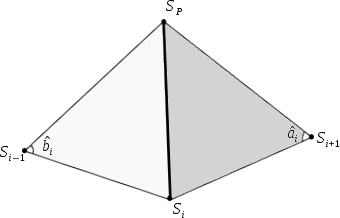
\includegraphics[width=150pt]{imagens_malhas_moveis/curvatura_media.png}
  \caption{\footnotesize{Variáveis da fórmula da curvatura média.
}}
  \label{fig_curvatura_media}
\end{figure}

Em seu trabalho, \citeonline{Ohtake2003} apresentam uma suavização de malha baseada na difusão linear das retas normais da malha. Apresentam-se resultados comparativos do método proposto, chamado filtragem média iterativa nas retas normais ({\it iterative mean filtering on mesh normals}), com a suavização laplaciana simplificada, com a suavização baseada no fluxo médio da curvatura, conforme \citeonline{Desbrun1999}, com a suavização de \citeonline{Taubin1995, Taubin1995A} e com a suavização bi-laplaciana, conforme \citeonline{Kobbelt1998}. Comparou-se com esses métodos, pois, segundo \citeonline{Ohtake2003}, esses métodos provém ao usuário uma combinação de simplicidade, eficiência e velocidade e, consequentemente, são amplamente utilizados em diversas aplicações de modelagem geométrica. O método proposto foi o mais lento porém,  apresentou bons resultados em relação a características nítidas de formas com ruídos ({\it denoising shapes}). 

\citeonline{Freitag1997} combinou a suavização laplaciana com uma suavização baseada em otimização. Nesse trabalho, definiu-se uma suavização chamada ``suavização laplaciana inteligente'' ({\it smart laplacian smoothing}), em que realoca-se os vértices da malha apenas se houve alguma melhora da qualidade local da malha de acordo com alguma métrica de qualidade. Nas técnicas de suavização baseadas em otimização, para encontrar a nova posição do vértice, objetiva-se maximizar a função composta $F(S_{P}) = \min G_i(S_{P})$, para $0<i<n$, em que $n$ é o número de vértices e a função $G_i$ é uma métrica de qualidade. Realizam-se experimentos numéricos para comparar métricas de qualidade e custo computacional dos métodos propostos em duas e três dimensões.

\citeonline{Vartziotis2013} realizam comparações de um método proposto com a suavização laplaciana em que $\omega_i = A_i$, em que $A_i$ é a área do triângulo $i$, conforme \citeonline{Jones1974}; com a suavização laplaciana inteligente, conforme \citeonline{Freitag1997}; e com um método de otimização global, conforme \citeonline{Brewer2003, Zhang2005, Diachin2006}. O novo  método é chamado de método de transformações de elemento geométrico ({\it geometric element transformation method} - GETMe), e baseia-se na técnica de regularização de transformações de elemento, conforme \citeonline{Knupp2001, Diachin2006}. Nessa proposta, realiza-se o movimento avaliando duas métricas de qualidade de malha $q_{min}$ e $q_{mean}$, em que $q_{min} \leftarrow \min q(E_{i})$ e $q_{mean} \leftarrow \frac{1}{m} \sum_{i=1}^{m}q(E_{i})$, $i = [1,m]$, que representam, respectivamente, o elemento de qualidade mínima e a média da qualidade dos elementos, em que $E_{i}$ é um elemento da malha,. As novas posições são definidas como médias ponderadas, conforme  $S_{P}^{n+1} = \frac{ \sum_{i=1}^{m} \omega_{i}(S_{i}^{n+1} - S_{P}^{n+1}) } { \sum_{i=1}^{m} \omega_{i} }$, de forma que $\omega_{i} \leftarrow [1 - q(E_{i})]^k$, em que $k \geq 0$ é um parâmetro fixo de amplificação. Trata-se de um método de suavização baseado em otimização. Essa técnica é aplicada de forma iterativa até que as melhorias estejam abaixo de um determinado limiar.

Outros trabalhos que utilizam movimento de vértices baseado no laplaciano, alguns apresentando comparações com  o bi-laplaciano, conforme \citeonline{Kobbelt1998}, e o método de \citeonline{Taubin1995, Taubin1995A}, podem ser verificados em \citeonline{Freitag1997a, Vollmer1999, Soni2000, Schneider2001, Ohtake2000, Kim2004, Lange2005}.

\subsubsection{Trabalhos que realizam movimento de vértices baseado na formulação laplaciana}
\label{trabalhos_laplacianos}

Nesta subseção, apresentam-se alguns trabalhos que realizam o movimento de vértices, por meio da adaptatividade-{\it r}, baseado na formulação laplaciana. Nesses trabalhos, movimentam-se os vértices a fim de se obter melhorias na aproximação da solução da EDP.

Dentre as diversas variações desenvolvidas, segundo \citeonline[p. 57 - 58]{Thompson1999}, existe uma forma típica, conforme a equação $S_{P}^{n+1} = S_{P}^{n} + \beta \frac{ \sum_{i=1}^{m} \omega_{P,i}(S_{i}^{n} - S_{P}^{n}) } { \sum_{i=1}^{m} \omega_{P,i} }$, em que se calcula $\omega_{P,i}$ conforme $\omega_{P,i} = \iota \left| \frac { \phi_{i} - \phi_{P} } {\phi_{i} + \phi_{P}} \right|$, em que $\phi$ é o parâmetro adaptativo e $ 0 < \iota < 1$ é uma constante de intensidade de $\omega$. 

\citeonline{Littlefield2001} descreve um método explícito de elementos finitos de adaptatividade {\it r}, para aplicações de alto impacto e penetração. O esquema de adaptatividade {\it r} implementado nesse trabalho realiza o movimento baseado na suavização laplaciana e é semelhante à aplicação ALE, de forma que o movimento dos vértices é restrido aos limites físicos do material. A reconstrução da malha é realizada de forma local.

\citeonline{Shontz2006} realizam um estudo de movimento dos vértices em que se objetiva determinar, a partir da malha inicial, um conjunto de pesos locais para cada nó interior em função de seus vizinhos. Esses pesos são calculados usando uma matriz de rigidez dos elementos finitos. Nesse trabalho, utiliza-se um método chamado suavização laplaciana ponderada linear ({\it Linear Weighted Laplacian Smoothing - LWLS}).

\citeonline{Rajagopal2006} realizam uma avaliação de algoritmos de adaptatividade {\it r} com base no método de forças configuracionais e analogia a molas.  A avaliação é feita com base em aspectos qualitativos e quantitativos de estimativas de erro. O método proposto de adaptação da malha é baseado no método de força de configuracional em conjunto com o movimento baseado na suavização laplaciana ponderada e melhoria da malha através do refinamento {\it h}, baseado no erro de discretização. Os estudo numéricos confirmam que a proposta de adaptação {\it rh} é mais eficiente do que uma abordagem puramente {\it h} e mais flexível do que uma abordagem puramente {\it r}, com melhores características de convergência.

Um sistema adaptativo {\it rh}, proposto por \citeonline{Rajagopal2007}, foi formulado para analisar problemas de interface bi-materiais, utilizando o método dos elementos finitos. Trata-se de um combinação da força configuracional de adaptação {\it r}, com movimento baseado na suavização laplaciana ponderada e melhoria da malha por refinamento {\it h}.

\citeonline{Popiolek2009} apresentam uma estratégia de malha adaptativa para simulação numérica de fluxos transientes incompressíveis com transferência de calor e transporte de massa. Emprega-se o método dos elementos finitos com malhas não estruturadas formadas por tetraedros.  A fim de obter resultados precisos, utilizam-se indicadores de erro, um esquema de refinamento e um processo de movimento baseado na suavização laplaciana inteligente ({\it smart laplacian smoothing}), conforme \citeonline{Freitag1997}.

\subsubsection{Resumo}
\label{cap_malhas_moveis_consideracoes_finais}

Nesta seção, abordou-se malhas móveis. Na subseção (\ref{cap_adaptatividade}), diferentes tipos de adaptatividade de malhas foram apresentados, com ênfase nos métodos de malhas móveis. Também foi abordado o princípio de equidistribuição, na subseção (\ref{cap_principio_equidistribuicao}), com apresentação de um exemplo unidimensional. 

Comentou-se sobre o problema de computar soluções de EDPs, na subseção (\ref{cap_computacao_malhas_moveis}), utilizando malhas móveis. Ainda, na subseção (\ref{cap_revisao_metodos_malhas_moveis}), foram citados alguns trabalhos sobre malhas móveis desenvolvidos recentemente. Na subseção (\ref{cap_movimento_laplaciano}), apresentaram-se trabalhos que realizam melhorias na qualidade da malha por meio da suavização laplaciana e, na seção (\ref{trabalhos_laplacianos}), trabalhos que realizam o movimento dos vértices baseado na formulação laplaciana, com o intuito de obter melhorias na aproximação da solução da EDP.

\subsection{Métrica geométrica da qualidade da malha}
\label{cap_metrica_geometrica}

\citeonline{Bank97} propõem um algoritmo de suavização e utilizam uma métrica geométrica. Considere $\delta$ o triângulo da figura (\ref{fig_medida_t}), com vértices $v_1$, $v_2$ e $v_3$ e os vetores $ l_1 = \left[ \begin{array}{c}  x_3 - x_2 \\  y_3 - y_2 \end{array} \right ]$, $l_2 = \left[ \begin{array}{c}  x_1 - x_3 \\  y_1 - y_3 \end{array} \right ]$ e $l_3 = \left[ \begin{array}{c}  x_2 - x_1 \\  y_2 - y_1 \end{array} \right ]$, orientados em sentido anti-horário. A medida geométrica, utilizada por \citeonline{Bank97}, chamada {\it Shape Regularity Quality} (SRQ), denotada por $\upsilon(\delta)$, é dada por $\upsilon(\delta) = \frac {4 \sqrt{3}|\delta|} {|l_1|^2 + |l_2|^2 + |l_3|^2}$, em que $2|\delta| = (x_2 - x_3)(y_3 - y_1) - (x_3 - x_1)(y_2 - y_1)$, com os vértices orientados em sentido anti-horário. Caso estejam orientados em sentido horário, o valor de $|\delta|$ será negativo. Trata-se da razão entre a área do triângulo e a soma dos quadrados dos comprimentos das arestas. A constante $4\sqrt{3}$ é utilizada como fator de normalização, para que os valores fiquem entre $0 < \upsilon(\delta) < 1$. Para um triângulo equilátero, $\upsilon(\delta) = 1$, e para triângulos com ângulos muito pequenos será próximo a zero. Para entender o significado geométrico dessa medida, verifique \citeonline{Bank97}. Dada uma malha $M$, a medida SRQ dessa malha é dada pelo menor valor dessa métrica, denominado $\upsilon(\delta)_{min}$.

\begin{figure}[!ht]
  \centering
  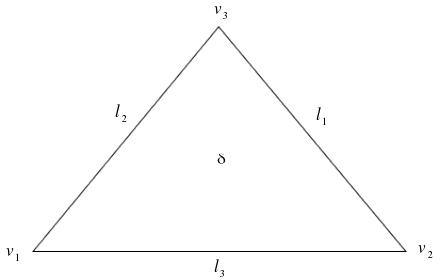
\includegraphics[width=150pt]{imagens_malhas_moveis/medida_t.png}
  \caption{\footnotesize{Rótulos e orientação do triângulo $\delta$.
}}
  \label{fig_medida_t}
\end{figure}

Segundo \citeonline{Bank97}, o único triângulo para o qual $\upsilon (\delta) = 1$ é o triângulo equilátero. Para $\frac{ \sqrt{3} } {2} \leq \upsilon(\delta) \leq 1$ tem-se triângulos sem ocorrência de ângulos obtusos. Conforme $\upsilon(\delta)$ é reduzido, o triângulo $\delta$ se torna mais degenerado.
 

\section{DESCRIÇÃO DO PROJETO COMPUTACIONAL PARA A SOLUÇÃO DA EQUAÇÃO DE CONDUÇÃO DO CALOR}
\label{cap:desenvolvimento}

Neste capítulo, descreve-se o projeto computacional para a solução de equações diferenciais parciais (EDPs) por discretizações por volumes finitos com refinamento de Delaunay e malhas móveis. Na seção (\ref{cap_aritmetica_precisão_arbitraria}), trata-se de apresentar a biblioteca de aritmética de precisão arbitrária e os motivos que levaram à sua escolha. Na seção (\ref{cap_malha_inicial}),  explica-se como é criada a triangulação inicial. Na seção (\ref{cap_refinamento_adaptativo}), descreve-se o procedimento de refinamento adaptativo, detalhando como é feita a seleção dos triângulos localizados nas regiões de grande variação. Apresenta-se um pseudocódigo desses procedimentos. Na seção (\ref{cap_resolucao_malha_inicial}), descreve-se como é realizada a resolução da malha inicial. Na seção (\ref{cap_movimento_vertices}), expõe-se o procedimento que realiza o movimento dos vértices entre as variações temporais da EDP, a função monitora escolhida e o critério de parada. Também apresenta-se um pseudocódigo desse procedimento. Todo o código foi implementado utilizando a linguagem de programação C++.

\subsection{Aritmética de precisão arbitrária}
\label{cap_aritmetica_precisão_arbitraria}

Preliminarmente, com o intuito de reduzir erros numéricos, verificou-se que seria necessário utilizar uma biblioteca para aritmética de precisão arbitrária. Dentre as diversas opções disponíveis, há a  {\it GNU Multiple-Precision Library}, também conhecida como GMP, que é uma biblioteca de código aberto para aritmética de precisão arbitrária, trabalhando sobre inteiros, racionais e números de ponto flutuante. Essa biblioteca permite que variáveis tenham um tamanho de bytes variável. Detalhes sobre a GMP podem ser verificados em \citeonline{GMP2012}. 

Outra opção, baseada na GMP, é a {\it Multiple-Precision Floating-point computations with correct Rounding} (MPFR). Essa biblioteca possui um conjunto maior de funções em comparação com a GMP, em especial funções transcendentais como exponenciais, logaritmos e funções trigonométricas, e valores especiais, como zeros assinados, infinitos e indicando o que não é um número - NaN. Além disso, a MPFR fornece um argumento adicional para as suas funções, em que se define o arredondamento utilizado, conforme especificado pelo padrão IEEE 754-200  \footnote{Disponível em http://ieeexplore.ieee.org/stamp/stamp.jsp?tp=\&arnumber=4610935 }. 

Neste trabalho, o parâmetro utilizado em todas as operações especifica o arredondamento ``{\it round to nearest}``, em que, ao realizar o arredondamento, o {\it bit} menos significativo é definido para zero. Conforme \citeonline{MPFR2007}, utilizando a MPFR é garantido que o resultado de qualquer operação seja o valor de ponto flutuante mais próximo possível do resultado exato. Maiores informações sobre a MPFR podem ser encontradas em \citeonline{MPFR2007}. Ainda, optou-se por utilizar uma interface da MPFR para C++, chamada {\it mpfr::real} \footnote{Disponível em: http:://chschneider.eu/programming/mpfr\_real/}, publicada sob os termos da GNU GPL v3  \footnote{Disponível em: http://www.gnu.org/licenses/}, que minimiza as alterações necessárias no código para utilizar a biblioteca para aritmética de precisão arbitrária MPFR.

\subsection{Criação da malha inicial}
\label{cap_malha_inicial}

Ao executar o código, inicialmente, lê-se um arquivo de entrada contendo os vértices iniciais da triangulação. O domínio é dividido em dois triângulos, formados pelos vértices situados na fronteira do domínio. A malha inicial, formada pelos vértices do arquivo de entrada, é criada utilizando o algoritmo de \citeonline{Green1978}, conforme o algoritmo (\ref{algoritmo_green_sibson}) apresentado na seção (\ref{cap_algoritmo_green_sibson}), na página \pageref{cap_algoritmo_green_sibson}. Neste trabalho, para geração da malha inicial, utilizou-se o projeto computacional criado para as simulações publicadas em \citeonline{TallesSanderson2012}.

A malha inicial gerada conterá triângulos de Delaunay em todo o domínio que envolve o \emph {Planar Straight Line Graph} (PSLG). Este algoritmo recebe como entrada um PSLG, permitindo arestas pendentes e pontos isolados, tendo apenas a restrição de que todos os ângulos presentes no PSLG sejam, de pelo menos, $60^{\circ}$. Dessa forma, tem-se a triangulação inicial, formada pelos vértices do arquivo de entrada. Com a malha inicial gerada, pode-se realizar o refinamento adaptativo.

\subsection{Refinamento de Delaunay}
\label{cap_refinamento_adaptativo}

Executam-se os algoritmos de \citeonline{Ruppert1995} e, em seguida, o de \citeonline{Ungor2004, Ungor2009}, cujos códigos-fonte foram criados pelo projeto computacional desenvolvido por \citeonline{TallesSanderson2012a}. Neste, trabalho realiza-se o refinamento de Delaunay seguindo dois critérios, que são explicados a seguir, até que o número mínimo de vértices, denotado por $\chi$, seja atingido. Apresentou-se o algoritmo de \citeonline{Ungor2004, Ungor2009} na subseção (\ref{cap_off_centers}), representado pelo algoritmo (\ref{algoritmo_ungor}), na página \pageref{algoritmo_ungor}. O número mínimo de vértices para a fase de refinamento é definido na subseção (\ref{comparativo_a}), página \pageref{comparativo_a}.

O primeiro critério, denotado por $\sigma$, definido automaticamente durante a execução, seleciona triângulos localizados em regiões de grande variação. Para isso, utiliza-se o gradiente, chamado aqui de $\gamma$. Para calcular $\gamma$, considere uma aresta $a$ de um determinado triângulo, formada pelos vértices $v_1$ e $v_2$. Calcula-se o módulo da diferença do valor $\phi$ da EDP nesses vértices, dividido pela distância que os separa. Com isso, tem-se que $\gamma_{a} = \frac{ | \phi_{v_1} - \phi_{v_2} | }{d_{( v_{1},v_{2} )}}$, em que $\phi_{v_1}$ é o valor da EDP no vértice $v_1$, $\phi_{v_2}$ é o valor da EDP no vértice $v_2$ e $d_{( v_{1},v_{2} )}$ é a distância que separa os vértices $v_1$ e $v_2$. 

No passo de refinamento adaptativo, em que se verifica se a quantidade mínima de vértices é alcançada, o valor do critério $\sigma$ é aumentado, de modo a selecionar triângulos localizados em regiões de maior variação em relação à iteração anterior. Ao se aumentar $\sigma$, seleciona-se menos arestas para o refinamento, mas somente arestas nas regiões de maior variação da solução. Para se definir o aumento de $\sigma$, calcula-se o maior e menor valor de $\gamma$ na malha, $\gamma_{max}$ e $\gamma_{min}$ respectivamente, e obtém-se a diferença entre esses valores. Essa diferença será multiplicada por uma constante $0 < \theta < 1$ de forma que, quanto menor o valor de $\theta$, mais triângulos serão selecionados por esse critério. Para os testes realizados, define-se o valor de $\theta$ na pág. \pageref{cap:resultados}, do capítulo (\ref{cap:resultados}). Dessa forma, a cada iteração do passo de refinamento adaptativo, atualiza-se $\sigma$, com seu valor inicial igual a zero, de forma que $\sigma \leftarrow \sigma + \theta( \gamma_{max} - \gamma_{min})$. Com isso, triângulos que foram refinados em uma iteração não serão selecionados na iteração posterior, pois o valor de $\gamma$ aumentou. Triângulos que contêm, pelo menos, uma aresta com $\gamma > \sigma$ serão refinados utilizando o algoritmo de \citeonline{Ruppert1995}, cujo código-fonte foi desenvolvido pela implementação em \citeonline{TallesSanderson2012}. 

O segundo critério refere-se ao ângulo mínimo $\alpha$, definido pelo usuário. Triângulos com ângulo mínimo menor que $\alpha$ serão refinados utilizando o algoritmo de \citeonline{Ungor2004, Ungor2009}, cujo código-fonte foi desenvolvido pela implementação de \citeonline{TallesSanderson2012a}. Em vez de se verificar o ângulo mínimo de cada triângulo, considera-se a métrica {\it Circunradius-to-shortest Edge Radio} (CER), explicada na subseção (\ref{cap_algoritmo_ruppert}), na página \pageref{cap_algoritmo_ruppert}, denotada por $\rho$. Como $\rho$ é inversamente proporcional ao ângulo, para uma boa qualidade geométrica, $\rho$ deve ser menor que $\rho_{\alpha}$, em que $\rho_{\alpha}$ é o valor da medida CER do ângulo $\alpha$. Com isso, refinam-se os triângulos com $\rho > \rho_{\alpha}$. Consequentemente, o maior valor da medida CER encontrado na malha, denotado por $\rho_{max}$, será tal que $\rho_{max} < \rho_{\alpha}$.

Dessa forma, tem-se o refinamento dos triângulos localizados nas regiões de grande variação, com uma qualidade mínima garantida pelo algoritmo de \citeonline{Ungor2004, Ungor2009}.

\subsection{Resolução da equação de condução do calor por discretizações de volumes finitos na malha inicial}
\label{cap_resolucao_malha_inicial}

Após realizar o refinamento adaptativo, executa-se o método dos volumes finitos (MVF), representado pelo algoritmo (\ref{algoritmo_metodo_volumes_finitos}) da subseção (\ref{cap_discretizacao_malha_irregular}), página \pageref{algoritmo_metodo_volumes_finitos}, a fim de gerar o sistema linear. Para solucionar a equação da condução de calor adaptou-se o código-fonte desenvolvido por \citeonline{TallesSanderson2012a} a fim de obter a solução da equação de Laplace por discretizações de volumes finitos. Considera-se que o valor da EDP, em todos os vértices internos, na iteração inicial no tempo, é igual a zero. 

Realiza-se o reordenamento da lista de vértices utilizando o algoritmo Cuthill-McKee reverso (CMr), conforme o algoritmo (\ref{algoritmo_cuthill_mckee}), introduzido na subseção (\ref{cap_cuthill_mckee_reverso}), página \pageref{algoritmo_cuthill_mckee}, com o vértice pseudoperiférico $\nu$ como vértice inicial, conforme o algoritmo (\ref{algoritmo_pseudo_periferico}), apresentado na mesma subseção, na página \pageref{algoritmo_pseudo_periferico}, cujo código-fonte foi desenvolvido na implementação de \citeonline{GuilhermeSanderson2013}. 

Executa-se o método dos gradientes conjugados (MGC) com precisão numérica $\epsilon$, cujo código-fonte foi desenvolvido na implementação de \citeonline{TallesSanderson2012a}, tal qual o algoritmo (\ref{algoritmo_gradiente_conjugado}), introduzido na subseção (\ref{cap_construcao}), página \pageref{algoritmo_gradiente_conjugado}, a fim de atualizar os valores da EDP em cada vértice, obtendo melhores resultados após o refinamento adaptativo. 

O processo para criação da malha inicial e refinamento adaptativo pode ser observado no algoritmo (\ref{malha_refinamento_adaptativo}). Os parâmetros de entrada do algoritmo (\ref{malha_refinamento_adaptativo}) são mostrados na tabela (\ref{tabelaParametrosEntrada}). O algoritmo 7 é apresentado conforme desenvolvido em \citeonline{GuilhermeSanderson2013}. A próxima etapa trata do movimento dos vértices, na subseção (\ref{cap_movimento_vertices}). 

\begin{algorithm}
\caption{ Método de geração e refinamento da malha.} 
\label{malha_refinamento_adaptativo}
\Entrada{Grafo $G=(L_V,L_E)$, em que $L_V$ é a lista dos v\'ertices e $L_A$ é a lista de arestas da triangulação inicial, $\alpha$, $\theta$, $\epsilon$, $\Delta t$ e $\chi$.  \CommentSty{// Verifique tabela (\ref{tabelaParametrosEntrada}).} }
\Saida{Solução inicial. \CommentSty{// Malha com \^angulos entre $\alpha$ e\\ // $\pi - 2 \alpha$, refinada nas regiões de grande varia\c{c}\~ao.} }
\Inicio{
  $\sigma \leftarrow 0$; \\
  \CommentSty{// Gera malha $M$, a partir de $L_V$.}  \\   
  $M \leftarrow AlgoritmoGreenSibson(L_V);$ \\ 
  \CommentSty{// Nas simula\c{c}\~oes, $\chi$ \'e definido na subse\c{c}\~ao\\ // (\ref{comparativo_a}), p\'agina \pageref{comparativo_a}.} \\
  \Enqto{ ($M.numeroVertices < \chi$ ) } 
  { \nllabel{laco_enquanto_inicio} 
      \CommentSty{// $\gamma_{max}$ e $\gamma_{min}$ são o maior e menor valor de $\gamma$ da\\ // malha, em que $\gamma$ \'e o gradiente.} \\           
      $\gamma_{max} \leftarrow calcula\gamma_{max}(M)$; \\
      $\gamma_{min} \leftarrow calcula\gamma_{min}(M)$; \\
      \CommentSty{// $\sigma$ \'e o crit\'erio de sele\c{c}\~ao de tri\^angulos\\ // para refinamento.} \\           
      $\sigma \leftarrow \sigma + \theta ( \gamma_{max} - \gamma_{min} )$; \\
      \CommentSty{// Refina triangulos com $\gamma > \sigma$.}  \\   
      $RefinaPorAlgoritmoRuppert(\sigma , M);$ \\
      \CommentSty{// Refina tri\^angulos com \^angulos menores que\\ // $\alpha$.}  \\ 
      $RefinaPorAlgoritmoUngor(\alpha, M);$ \\      
      \CommentSty{// Gera sistema linear pelo MVF.}  \\ 
      $MetodoVolumesFinitos(M, t \times \Delta t)$; \\
      \CommentSty{// Executa reordenação dos v\'ertices.}  \\
      $\nu \leftarrow AlgoritmoVerticePseudoPeriferico(M)$; \\
      $AlgoritmoCuthillMcKeeReverso(M, \nu);$ \\      
      \CommentSty{// Atualiza valores da EDP pelo MGC.}  \\       
      $MetodoGradientesConjugados(M, \epsilon)$; \\         
  } \nllabel{laco_enquanto_fim} 
}
\end{algorithm}

\begin{table}[!h!t!b]
\centering%fim da centralização da tabela
\vspace*{11pt}
\begin{tabularx}{\textwidth}{c c X}
\hline
Variável & Algoritmo &  Descrição \\
\hline %----- linha horizontal
$L$             & (\ref{malha_refinamento_adaptativo})                       & Lista de vértices e arestas da triangulação inicial de Delaunay. \\
$\theta$        & (\ref{malha_refinamento_adaptativo})                       & Constante quantificadora do critério de seleção para refinamento.  \\
$\chi$          & (\ref{malha_refinamento_adaptativo})                       & Número mínimo de vértices na malha. \\
$M$             & (\ref{malha_movel})                                        & Malha inicial gerada no algoritmo (\ref{malha_refinamento_adaptativo}). \\
$\beta$         & (\ref{malha_movel})                                        & Parâmetro que controla a amplitude do movimento dos vértices. \\
$\lambda$,$\mu$ & (\ref{malha_movel})                                        & Parâmetros de relaxamento específicos da função de \citeonline{Taubin1995, Taubin1995A}. \\
$\eta$          & (\ref{malha_movel})                                        & Valor de tolerância da métrica SRQ para continuar movimentando os vértices. \\
$t_{final}$     & (\ref{malha_movel})                                        & Número máximo de iterações temporais. \\
$\Delta t$      & (\ref{malha_refinamento_adaptativo}) e (\ref{malha_movel}) & Variação do tempo utilizado na discretização da equação do calor pelo MVF. \\
$\alpha$        & (\ref{malha_refinamento_adaptativo}) e (\ref{malha_movel}) & Ângulo mínimo utilizado para realizar refinamento. \\
$\epsilon$      & (\ref{malha_refinamento_adaptativo}) e (\ref{malha_movel}) & Precisão numérica do MGC. \\
\hline %----- linha horizontal
\end{tabularx}%--- fechamento do ambiente tabular
\caption{Descrição dos parâmetros de entrada dos algoritmos (\ref{malha_refinamento_adaptativo}) e (\ref{malha_movel}). Todas as variáveis são definidas pelo usuário via arquivo de configuração.} %legenda da tabela
\label{tabelaParametrosEntrada}
\end{table}

\subsection{Movimento dos vértices}
\label{cap_movimento_vertices}

O movimento dos vértices ocorre entre cada etapa de variação do tempo, referente à discretização da equação do calor. Entre cada etapa de variação do tempo optou-se por realizar o movimento dos vértices enquanto uma condição de qualidade geométrica da malha for satisfeita. Quando essa condição não for mais satisfeita, executa-se o algoritmo de \citeonline{Ungor2004, Ungor2009}, pela implementação desenvolvida por \citeonline{TallesSanderson2012a}, com o objetivo de melhorar a qualidade da malha. Essa métrica de qualidade geométrica será explicada mais adiante.

Definiu-se uma nova função monitora, chamada de $\Lambda$, baseada no laplaciano. Leva-se em consideração a maior diferença do valor da EDP em toda a malha entre vértices adjacentes. Para um vértice $P$, a função monitora $\Lambda$ fica $S_{P}' \leftarrow S_{P} + \frac {\beta} {\Delta \phi_{max} } \sum_{i=1}^{n} (S_i - S_P) (| \phi_i - \phi_P |)$, em que $S_P$ é a posição do vértice $P$, $0 < \beta < 1$ é um parâmentro para controle do movimento, $n$ é o número de vértices adjacentes a $P$, $\phi_i$ é o valor da EDP no vértice $i$, adjacente à $P$, $\phi_P$ é o valor da EDP no vértice $P$, $\Delta \phi_{max}$ é o maior valor de $| \phi_i - \phi_P|$, para toda aresta pertencente à malha e $S_P'$ é o valor da nova posição do vértice $P$. Essa função realiza movimentos mais rápidos nas regiões de maior variação, onde o $| \phi_i - \phi_P $| é próximo ao valor de $\Delta \phi_{max}$.

A função monitora $\Lambda$ é comparada com outras quatro funções, todas conforme $S_{P}' \leftarrow S_{P} + \beta  \frac { \Sigma_{i = 1}^{n} (S_{i} - S_{P}) \omega_{P,i} } { \Sigma_{i = 1}^{n}  \omega_{P,i}  }$, apresentadas na seção (\ref{cap_suavizacao_laplaciana}), página \pageref{cap_suavizacao_laplaciana}. As funções, escolhidas por serem consideradas clássicas na literatura, são as seguintes:

\begin{enumerate}
 \item Comparação com a função monitora baseada diretamente na formulação laplaciana, em que $\omega_{P,i} = { | \phi_{i} - \phi_{P} | }$. Essa função é aqui chamada de $\Gamma$;
 
 \item Comparação com uma função proposta por \citeonline{Taubin1995, Taubin1995A}, em que $\omega_{P,i} = { | \phi_{i} - \phi_{P} | }$, combinada por dois movimentos sucessivos, conforme tal que $S_{P}' = S_{P} + \lambda \Delta S_{P}$ e $S_{P}'' = S_{P}' - \mu \Delta S_{P}'$, em que $\Delta S_{P} =  \frac{ \sum_{i=1}^{m} \omega_{P,i}(S_{i}^{n} - S_{P}^{n}) } { \sum_{i=1}^{m} \omega_{P,i} }$ e os parâmetros de relaxamento $0 < \lambda < \mu$. Essa função é aqui chamada de $\Xi$, mas é conhecida como função $\lambda - \mu$. Esse esquema de duas combinações sucessivas foi utilizado no âmbito da suavização laplaciana em \citeonline{Taubin1995, Taubin1995A}. Na subseção (\ref{cap_movimento_laplaciano}), página \pageref{cap_movimento_laplaciano}, apresentam-se alguns trabalhos que utilizam essa função para melhoria da qualidade da malha. Não foram encontrados trabalhos em que se utilizou essa função como função monitora; 
 
 \item Comparação com a função monitora proposta por \citeonline{Taubin1995, Taubin1995A}, entretanto, configurada com $\lambda = \mu$, conforme proposto por \citeonline{Kobbelt1998}, conhecida como bi-laplaciana, chamada aqui de $\Psi$. Na subseção (\ref{cap_movimento_laplaciano}), página \pageref{cap_movimento_laplaciano}, apresentam-se trabalhos que utilizam essa função. Não foram encontrados trabalhos em que se utilizou essa função como função monitora;
 
 \item Comparação com a função definida por \citeonline[p. 57 - 58]{Thompson1999}, em que o peso $\omega_{P,i}$ é tal que $\omega_{P,i} = \iota \left( \frac { | \phi_{i} - \phi_{P} | } { | \phi_{i} + \phi_{P} | } \right) $, para $0 < \iota < 1$. Essa função é aqui chamada de $\Upsilon$.
\end{enumerate}

Os valores de $\beta$, $\lambda$, $\mu$ e $\iota$, utilizados nas funções monitoras, são definidos no capítulo (\ref{cap:resultados}).

Escolheram-se essas funções monitoras, pois são funções consideradas eficientes, graças à sua velocidade e simplicidade. São funções já concretizadas na literatura, clássicas, sendo utilizadas em diversos trabalhos comparativos, conforme apresentados nas subseções (\ref{cap_movimento_laplaciano}) e (\ref{trabalhos_laplacianos}). Além disso, quanto às funções de \citeonline{Taubin1995, Taubin1995A} e \citeonline{Kobbelt1998}, chamadas aqui respectivamente de $\Xi$ e $\Psi$, não foram encontrados trabalhos em que essas funções foram utilizadas a fim de obter melhorias na aproximação da solução da EDP. Optou-se também pela função de \citeonline{Thompson1999}, chamada aqui de $\Upsilon$, por apresentar bons resultados nos testes realizados e, além disso, segundo o autor, trata-se de uma típica abordagem.

Avaliou-se a possibilidade de movimentar os vértices, repetidamente, até que não houvesse mais movimento, em seguida, executar o algoritmo de \citeonline{Ungor2004, Ungor2009} e avançar a etapa de tempo. Entretanto, devido à alta precisão da biblioteca MPFR, experimentos mostraram que o movimento, ainda que pequeno, sempre ocorre. Ao se realizar testes em uma malha com 100 vértices, movimentando-a, incondicionalmente, ao atingir 400 iterações de movimento dos vértices, os valores das métricas de qualidade não variavam mais. No entanto, o movimento dos vértices ainda existia. 

O procedimento de movimento dos vértices repete-se enquanto a malha tiver uma qualidade geométrica mínima. A métrica {\it Shape Regularity Quality} (SRQ), descrita na subseção (\ref{cap_metrica_geometrica}), na página \pageref{cap_metrica_geometrica}, denotada  por $\upsilon$, é verificada. O valor de $\upsilon$ varia de zero a um e, quanto mais próximo de um, mais se assemelha a um triângulo equilátero. Então, movimenta-se a malha enquanto esta ainda tiver um valor satisfatório de $\upsilon$. Dessa forma, define-se um valor $0 < \eta < 1$ de forma que, o procedimento de movimento dos vértices é repetido enquanto $\upsilon_{min} > \eta$, em que $\upsilon_{min}$ é o menor valor da medida SRQ encontrado na malha. O valor de tolerância $\eta$ da métrica SRQ para continuar movimentando  os vértices é definido na página \pageref{cap:resultados}, do capítulo (\ref{cap:resultados}).

Com o término do procedimento de movimento dos vértices, executa-se o algoritmo de \citeonline{Ungor2004, Ungor2009} e avança-se uma iteração no tempo. O algoritmo de \citeonline{Ungor2004, Ungor2009} torna a malha uma triangulação de Delaunay, caso essa tenha deixado de ser, exceto se tiver ocorrido o emaranhamento das arestas, apresentando erros caso triângulos com essas arestas sejam selecionados para refinamento. Após avançar a etapa de tempo, executa-se o MVF, o algoritmo CMr com o vértice pseudoperiférico $\nu$ como vértice inicial e o MGC, com precisão numérica $\epsilon$. O procedimento para movimentar os vértices e realizar o refinamento de triângulos com $\measuredangle < \alpha$ pode ser observado no algoritmo (\ref{malha_movel}). Os parâmetros de entrada do algoritmo (\ref{malha_movel}) são mostrados na tabela (\ref{tabelaParametrosEntrada}), página \pageref{tabelaParametrosEntrada}. Por fim, verifica-se se houve o emaranhamento de arestas, por meio de um método que busca vértices dentro dos triângulos. Um método de força bruta mostrou-se demasiadamente demorado portanto, utilizou-se um método que verifica se os vértices vizinhos e os vizinhos desses encontram-se dentro do triângulo em questão.

\begin{algorithm}
\caption{ Método de movimento da malha (malha móvel).} 
\label{malha_movel}
\Entrada{Malha inicial $M$, $\alpha$, $\beta$, $\epsilon$, $\eta$, $\Delta t$ e $t_{final}$. \\ \CommentSty{ // Verifique tabela (\ref{tabelaParametrosEntrada}).} }
\Saida{Solução da equa\c{c}\~ao do calor por discretiza\c{c}\~oes de volunes finitos com diagrama de Voronoi.}
\Inicio{    
    $t \leftarrow 1;$ \CommentSty{// Para t=0, considera-se o algoritmo (\ref{malha_refinamento_adaptativo}).}  \\        
    \Enqto{ ($t \leq t_{final}$) } 
    {
	\Repita{ ($houveMov = falso$) ou ($\upsilon_{min} < \eta$) } 
	{ \nllabel{laco_repita_inicio}    
	    \CommentSty{// Movimenta a malha e calcula $\upsilon_{min}$}  \\   	    
	    $houveMov \leftarrow MovimentaMalha(\beta, M)$;  \nllabel{movimenta_malha}  \\
	    $ \upsilon_{min} \leftarrow ShapeRegularityQuality(M)$; \\
	    \Se { ($houveMov$ e $\upsilon_{min} \geq \eta$) } {    
	      \CommentSty{// Gera sistema linear pelo MVF.}  \\ 
	      $MetodoVolumesFinitos(M, t \times \Delta t)$; \\
	      \CommentSty{// Executa reordenação dos v\'ertices.}  \\
	      $\nu \leftarrow AlgoritmoVerticePseudoPeriferico(M)$; \\
	      $AlgoritmoCuthillMcKeeReverso(M, \nu);$ \\
	      \CommentSty{// Atualiza valores da EDP pelo MGC.}  \\ 
	      $MetodoGradientesConjugados(M, \epsilon)$; \\
	    }
	} \nllabel{laco_repita_fim}    
	\Se { ($\upsilon_{min} < \eta$) } {
	  \CommentSty{// Refina tri\^angulos com $\measuredangle < \alpha$.}  \\   	  
	  $RefinaPorAlgoritmoUngor(\alpha , M)$;  \CommentSty{ // se a malha\\ // deixou de ser uma triangulação de\\ // Delaunay, off-centers fará com que seja.}  \\	  
	}
	\Se { (houveMov)  } {
	  \CommentSty{// Gera sistema linear pelo MVF.}  \\ 
	  $MetodoVolumesFinitos(M, t \times \Delta t)$; \\	
	  \CommentSty{// Executa reordenação dos v\'ertices.}  \\
	  $\nu \leftarrow AlgoritmoVerticePseudoPeriferico(M)$; \\
	  $AlgoritmoCuthillMcKeeReverso(M, \nu)$; \\      		
	  \CommentSty{// Atualiza valores da EDP pelo MGC.}  \\ 
	  $MetodoGradientesConjugados(M, \epsilon)$; \\    	
        }	
	$t \leftarrow t + 1$; \CommentSty{// Avan\c{c}a a etapa de tempo.}  \\ 
	\CommentSty{// Gera sistema linear para etapa $t+1$.}  \\ 
	$MetodoVolumesFinitos(M, t \times \Delta t)$; \\
	\CommentSty{// Executa reordenação dos v\'ertices.}  \\
	$\nu \leftarrow AlgoritmoVerticePseudoPeriferico(M)$; \\
	$AlgoritmoCuthillMcKeeReverso(M, \nu)$; \\ 
	\CommentSty{// Atualiza valores da EDP para etapa $t+1$.}  \\ 
	$MetodoGradientesConjugados(M, \epsilon)$; \\ 
    }
}
\end{algorithm}  

Apesar de o algoritmo de \citeonline{Ungor2004, Ungor2009} utilizar a métrica CER, para se avaliar a qualidade da malha, utiliza-se a métrica SRQ no algoritmo (\ref{malha_movel}). Inicialmente, considerou-se a possibilidade de se utilizar também a métrica CER como critério de parada do movimento de vértices. Entretanto, para utilizar a métrica CER e para existir a possibilidade de movimentar a malha por sucessivas vezes com essa métrica, seria necessário criar uma malha com um ângulo mínimo de $32^{\circ}$, e movimentar a malha enquanto $\alpha_{min} > 30^{\circ}$, criando uma ``folga'' de $2^{\circ}$, por exemplo. Caso contrário, cada função seria executada uma só vez. A utilização da SRQ permitiu que o movimento de malhas com uma função monitora pudesse ser executado sucessivas vezes, sem haver emaranhamentos da malha.


\subsection{Resumo}
\label{cap_consideracoes_finais}

Nesse capítulo, apresentou-se a biblioteca de aritmética de precisão arbitrária MPFR e os motivos que levaram à sua escolha. Também elucidou-se como é criada a triangulação de Delaunay inicial, o refinamento adaptativo e o procedimento que realiza o movimento dos vértices. 

Definiu-se uma nova função monitora, denotada $\Lambda$. Também esclareceu-se como é realizado o movimento dos vértices enquanto atender um critério de qualidade mínima, definido por uma métrica de qualidade geométrica. Outras funções monitoras foram apresentadas, que serão comparadas com a função monitora $\Lambda$. Também apresentam-se pseudocódigos de todos os procedimentos.

\section{TESTES EXPERIMENTAIS E DISCUSSÃO DOS RESULTADOS}
\label{cap:resultados}

Este capítulo tem o objetivo de apresentar os resultados dos experimentos realizados. Os detalhes referentes à implementação foram elucidados no capítulo (\ref{cap:desenvolvimento}) portanto, os detalhes das variáveis e dos algoritmos citados também se encontram nesse capítulo. Utiliza-se uma precisão de cinco casas decimais na exibição dos resultados e, para valores menores que $10^{-3}$ ou valores grandes, emprega-se a notação científica, de forma que $1e-4 = 0,0001$.

Os experimentos numéricos foram realizados utilizando o sistema operacional Ubuntu 12.04 LTS 64 bits, processador Intel(R) i3 de 3.10GHz e memória de 16Gb. De modo a se obter soluções em tempo hábil e que atendesse a precisão possível de acordo com a memória disponível, utilizou-se 512 bits de precisão na configuração da biblioteca {\it Multiple-Precision Floating-point computations with correct Rounding}. Os resultados descritos aqui são uma seleção representativa de um grande número de experimentos.

O domínio discretizado nos experimentos trata-se de um quadrado, de dimensões $50 \times 50$, com o valor das condições de fronteira nas faces leste, oeste e sul igual a dez, e na face norte, igual a zero. A estimativa inicial da equação diferencial parcial (EDP), em todos os vértices internos, na iteração inicial no tempo, é igual a zero. 

Quanto às variáveis da tabela (\ref{tabelaParametrosEntrada}), mostrada na página \pageref{tabelaParametrosEntrada}, definiram-se dez iterações no tempo, denotadas por $t$, tal que $t_{final} = 10$, com uma variação $\Delta t = 0,1$. O ângulo mínimo $\alpha$, conforme a subseção (\ref{cap_algoritmo_ruppert}), página \pageref{cap_algoritmo_ruppert}, é definido para $\alpha = 30^{\circ}$ com $\rho_{\alpha} = 1,0$. Essa escolha do valor de $\alpha$ se deve por estar próximo dos limites práticos do algoritmo de refinamento. O parâmetro de refinamento adaptativo $\theta$, definido na subseção (\ref{cap_refinamento_adaptativo}), página \pageref{cap_refinamento_adaptativo}, é tal que $\theta = 1e-10$, tornando menos brusca a diferença na proporção dos triângulos. A precisão numérica $\epsilon$ do métodos dos gradientes conjugados é $\epsilon = 1e-10$, com o intuito de obter uma precisão aceitável dos resultados,  minimizando o número de iterações desse método, conforme observado no algoritmo (\ref{algoritmo_gradiente_conjugado}), apresentado na subseção (\ref{cap_construcao}), página \pageref{algoritmo_gradiente_conjugado}. O movimento da malha é repetido enquanto $\upsilon_{min} > \eta$ tal que o valor $\eta = 0,6$, em que ambos os valores de $\upsilon_{min}$ e $\eta$ denotam os valores da métrica {\it Shape Regularity Quality} (SRQ), apresentados, respectivamente, na subseção (\ref{cap_metrica_geometrica}), página \pageref{cap_metrica_geometrica} e na subseção (\ref{cap_movimento_vertices}), página \pageref{cap_movimento_vertices}. A escolha desse valor de $\eta$ é devido ao limite do algoritmo de \citeonline{Ungor2004, Ungor2009}, que consegue gerar malhas com ângulo mínimo próximo à $32^{\circ}$. Os experimentos mostraram que malhas geradas pelo algoritmo (\ref{malha_refinamento_adaptativo}), configuradas com $\eta = 0,6$ e $\alpha = 30^{\circ}$ possuem $\upsilon_{min} = 0,6$ e $\rho_{max} = 1$

Para todas as funções monitoras, realizam-se comparações, apresentadas nas próximas subseções, para diferentes malhas, utilizando o parâmetro de adaptatividade $\beta = 0,1$, $\beta = 0,2$, $\beta = 0,3$, $\beta = 0,4$, $\beta = 0,5$ e $\beta = 0,6$. Os valores dessas variáveis estão resumidos na tabela (\ref{tabelaValorParametros}). Nos experimentos utilizando $\beta = 0,6$ no entanto, ocorreram emaranhamentos na função $\Lambda$. Nos resultados apresentados, em que é informado que utilizou-se $\beta = 0,1$, equivale a $\lambda = 0,1$ e $\mu = 0,1001$, na função $\Xi$, e $\lambda = \mu = 0,1$ na função $\Psi$. Ao informar que utilizou-se $\beta = 0,2$, equivale a $\lambda = 0,2$ e $\mu = 0,2001$, na função $\Xi$, e $\lambda = \mu = 0,2$, na função $\Psi$, e assim suscessivamente.

\begin{table}[!h!t!b]
\centering
\vspace*{11pt}
 \begin{tabularx}{\textwidth}{c c X}
\hline
Variável & Algoritmo & Valor \\
\hline
$L_V$             & (\ref{malha_refinamento_adaptativo}) & {\small $v_0 = (0,0), v_1 = (50,0), v_2 = (0,50), v_3 = (50,50),$} \\
                  &                                      & {\small $v_4 = (10,10), v_5 = (25,25), v_6 = (40,40)$}\\
$L_A$             & (\ref{malha_refinamento_adaptativo}) & $(v_0, v_1), (v_0,v_2), (v_3,v_2), (v_3, v_1)$ \\
$\theta$          & (\ref{malha_refinamento_adaptativo}) & 1e-10 \\
$\chi$            & (\ref{malha_refinamento_adaptativo}) & 15.000, 30.000, 60.000 e 100.000 \\
$\beta$           & (\ref{malha_movel}) & 0,1, 0,2, 0,3, 0,4, 0,5 e 0,6 \\
$\lambda_{\Psi}$  & (\ref{malha_movel}) & 0,1, 0,2, 0,3, 0,4, 0,5 e 0,6 \\
$\lambda_{\Xi}$   & (\ref{malha_movel}) & 0,1, 0,2, 0,3, 0,4, 0,5 e 0,6 \\
$\mu_{\Psi}$      & (\ref{malha_movel}) & 0,1, 0,2, 0,3, 0,4, 0,5 e 0,6 \\
$\mu_{\Xi}$       & (\ref{malha_movel}) & 0,1001, 0,2001, 0,3001, 0,4001, 0,5001 e 0,6001\\
$\iota$           & (\ref{malha_movel}) & 1 \\
$\eta$            & (\ref{malha_movel}) & 0,6 \\
$t_{final}$       & (\ref{malha_movel}) & 10 \\
$\Delta t$        & (\ref{malha_refinamento_adaptativo}) e (\ref{malha_movel}) & 0,1 \\
$\alpha$          & (\ref{malha_refinamento_adaptativo}) e (\ref{malha_movel}) & $30^{\circ}$\\
$\epsilon$        & (\ref{malha_refinamento_adaptativo}) e (\ref{malha_movel}) & 1e-10\\
\hline %----- linha horizontal
\end{tabularx}
\caption{Valores das variáveis referentes ao parâmetros de entrada dos algoritmos (\ref{malha_refinamento_adaptativo}) e (\ref{malha_movel}) .} %legenda da tabela
\label{tabelaValorParametros}
\end{table}


O grafo $G = (L_V,L_E)$, que representa o {\it Planar Straight Line Graph}, contém o conjunto de vértices $L_V$, formado por $v_0 = (0,0), v_1 = (50,0), v_2 = (0,50), v_3 = (50,50), v_4 = (10,10), v_5 = (25,25)$ e $v_6 = (40,40)$, e o conjunto de arestas $L_E $, formado por $\{(v_0, v_1), (v_0,v_2), (v_3,v_2), (v_3, v_1)\}$. Quanto aos parâmetros exclusivos de algumas funções monitoras, que quantificam o movimento, na função $\Upsilon$ utilizou $\iota = 1$. Na função $\Xi$, realiza-se experimentos com $\lambda = 0,1$ e $\mu = 0,1001$, $\lambda = 0,2$ e $\mu = 0,2001$, $\lambda = 0,3$ e $\mu = 0,3001$, $\lambda = 0,4$ e $\mu = 0,4001$, $\lambda = 0,5$ e $\mu = 0,5001$ e $\lambda = 0,6$ e $\mu = 0,6001$. Na função, $\Psi$, utiliza-se $\lambda = \mu = 0,1$, $\lambda = \mu = 0,2$, $\lambda = \mu = 0,3$, $\lambda = \mu = 0,4$, $\lambda = \mu = 0,5$ e  $\lambda = \mu = 0,6$ mostrados na subseção (\ref{cap_movimento_vertices}), página \pageref{cap_movimento_vertices}. Esses valores se encontram resumidos na tabela (\ref{tabelaValorParametros}). Para diferenciar os valores de $\lambda$ e $\mu$ das funções $\Xi$ e $\Psi$, são denotados na tabela (\ref{tabelaValorParametros}), respectivamente, por $\lambda_{\Xi}$, $\lambda_{\Psi}$, $\mu_{\Xi}$ e $\mu_{\Psi}$. Em outros trabalhos, conforme mencionado na subseção (\ref{cap_suavizacao_laplaciana}), página \pageref{cap_suavizacao_laplaciana}, utiliza-se $\lambda = \mu= 1$ na função bi-laplaciana entretanto, nos testes realizados com esse valor ocorreu o emaranhamento das arestas, por isso optou-se por utilizar esses valores de $\lambda$ e $\mu$.

Para que se possa comparar visualmente as diferenças de movimento entre as funções monitoras, criou-se uma malha por refinamento adaptativo, conforme o pseudocódigo (\ref{malha_refinamento_adaptativo}), com 3.841 vértices e avançou-se dez iterações temporais, movimentando os vértices conforme o pseudocódigo (\ref{malha_movel}), sob as condições de configuração mencionadas nesta subseção. Exemplos de malhas geradas após o movimento, guiado pelas funções monitoras $\Lambda$, $\Gamma$, $\Xi$, $\Psi$ e $\Upsilon$ podem ser visualizadas na figura (\ref{fig_comparacao_movimentos}).

\begin{figure}[!ht]
  \centering
  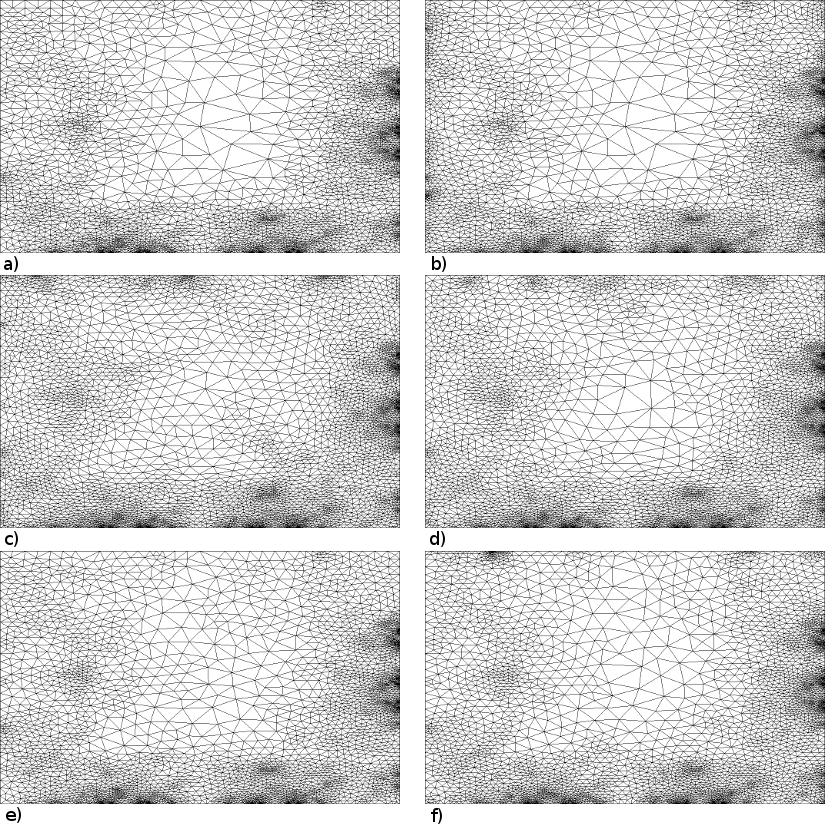
\includegraphics[width=400pt]{imagens_resultados/comparacao_movimentos.png}
  \caption{\footnotesize{Em a) malha inicial com 3.841 vértices. Em b), malha final movimentada pela função $\Lambda$; em c), pela função $\Gamma$; em d), pela função $\Xi$, em e), pela função $\Psi$ e em f), pela função $\Upsilon$.
}}
  \label{fig_comparacao_movimentos}
\end{figure}

Nas próximas subseções, apresenta-se os resultados comparativos entre as funções monitoras $\Lambda$, $\Gamma$, $\Xi$, $\Psi$ e $\Upsilon$.

\subsection{Comparativo funções monitoras}
\label{comparativo_a}

As malhas, geradas pelo algoritmo (\ref{malha_refinamento_adaptativo}), que foi configurado com número mínimo de vértices $\chi = 15.000$, $\chi = 30.000$, $\chi = 60.000$ e $\chi = 100.000$, possuem, respectivamente, um total de $15.788$, $32.515$, $67.963$ e $142.253$ vértices. Todas as malhas possuem, inicialmente, as métricas de qualidade $\rho_{max} = 1,0$ e $\upsilon_{min} = 0,6$. Na etapa temporal $t=1$, previamente ao se movimentar os vértices, o maior valor de $\gamma$, denotado $\gamma_{max}$, e o valor médio de $\gamma$, denotado $\gamma_{mean}$, das malhas geradas, encontram-se resumidos na tabela (\ref{tabela_malha_inicial}). O valor de $\gamma_{mean}$ tende a diminuir ao avançar a etapa temporal. A cada iteração do laço enquanto, linhas \ref{laco_enquanto_inicio} a \ref{laco_enquanto_fim}, do algoritmo (\ref{malha_refinamento_adaptativo}) aumenta-se o valor de $\gamma_{mean}$, inserindo-se novos vértices nas regiões de maior variação. Realizar o movimento dos vértices em direção à região de maior variação também aumenta o valor de $\gamma_{mean}$.

\begin{table}[!ht]
\begin{center}
 %aqui centralizamos a tabela
\begin{tabular}{|l|l|l|l|l|} %-----dividir em sete colunas
\hline
$\chi$ & 15.000 & 30.000 & 60.000 & 100.000 \\
\hline %----- linha horizontal
 $\gamma_{max}$    & 30,25185 & 30,91983 & 45,65052 &  65,18423\\
 $\gamma_{mean}$   & 3,08635 & 3,58712 & 4,08809 &  4,47127\\
\hline %----- linha horizontal
\end{tabular}%--- fechamento do ambiente tabular
\end{center}
 %fim da centralização da tabela
\caption{Valores de $\gamma_{max}$ e $\gamma_{mean}$, respectivamente, o maior valor de $\gamma$ e o valor médio de $\gamma$, na etapa temporal $t=1$.} %legenda da tabela
\label{tabela_malha_inicial}
\end{table}

\begin{sidewaystable}
% \scalefont{0.7}
\begin{center}
 %aqui centralizamos a tabela
\begin{tabular}{|c|l|r|r|r|r|r|r|r|} %-----dividir em sete colunas
\hline
& Função & $\Lambda$ & $\Gamma$ & $\Xi$ & $\Psi$ & $\Upsilon$ & S/Mov.1 & S/Mov.2 \\
\hline %----- linha horizontal
\multirow{5}{*}{\begin{sideways}$\chi = 15.000$\end{sideways} } 
& Total de vértices                                                     & 16.255 & 16.618 & 16.615 & 16.481 & 17.060 & 15.788 & 32.515 \\
& {\it Clocks} exp.	                                             	& 5,34e10 & 1,78e10 & 6,71e10 & 6,43e10 & 2,71e10 & 1,33e09 & 4,05e09 \\
& {\it Clocks} para mov.                                      		& 6,00e09 & 1,32e09 & 9,08e09 & 8,62e09 & 2,84e09 & - & - \\
& Rep. linhas \ref{laco_repita_inicio}-\ref{laco_repita_fim} 		& 163 & 24 & 344 & 267 & 49 & - & - \\
& Valor $\gamma_{max}$							& 128,89 & 26,39 & 26,26  & 26,21 & 180,42 & 26,13 & 36,13 \\
& Valor $\gamma_{mean}$							& 1,02420 & 0,99315 & 0,99602 & 0,99759 & 0,99436& 0,98318 & 1,03107 \\
\hline %----- linha horizontal
\multirow{5}{*}{\begin{sideways}$\chi = 30.000$\end{sideways} } 
& Total de vértices                                                     & 33.034 & 33.790 & 33.755 & 33.551 & 33.908 & 32.515 & 67.963 \\
& {\it Clocks} exp.	                                             	& 1,03e11 & 5,12e10 & 1,33e11 & 1,23e11 & 6,25e10 & 4,05e09 & 1,53e10 \\
& {\it Clocks} para mov.                                      		& 7,97e09 & 2,96e09 & 1,35e10 & 1,19e10 & 4,27e09 & - & - \\
& Rep. linhas \ref{laco_repita_inicio}-\ref{laco_repita_fim} 		& 105 & 26 & 291 & 183 & 37 & - & - \\
& Valor $\gamma_{max}$							& 50,36 & 51,24 & 50,21  & 49,43 & 111,51 & 36,13 & 52,37 \\
& Valor $\gamma_{mean}$							& 1,06513 & 1,05096 & 1,05477 & 1,05560 & 1,05921 & 1,03107 & 1,06202 \\
\hline %----- linha horizontal
\multirow{5}{*}{\begin{sideways}$\chi = 60.000$\end{sideways} } 
& Total de vértices                                                     & 68.840& 70.224 & 69.926 & 70.076 & 70.498 & 67.963 & 142.253 \\
& {\it Clocks} exp.	                                             	& 2,84e11 & 1,48e11 & 3,36e11 & 3,51e11 & 1,51e11 & 1,53e10  & 5,30e10 \\
& {\it Clocks} para mov.                                      		& 1,69e10 & 6,49e09 & 2,43e10 & 2,60e10 & 6,81e09 & - & - \\
& Rep. linhas \ref{laco_repita_inicio}-\ref{laco_repita_fim} 		& 109 & 27 & 180 & 215 & 31 & - & - \\
& Valor $\gamma_{max}$							& 177,60 & 49,47 & 52,24 & 52,35 & 174,41 & 52,37 & 72,37 \\
& Valor $\gamma_{mean}$							& 1,12378 & 1,09497 & 1,09474 & 1,09483 & 1,09755 &  1,06202 & 1,11495 \\
\hline %----- linha horizontal
\multirow{5}{*}{\begin{sideways}$\chi = 100.000$\end{sideways} } 
& Total de vértices                                                     & 143.107 & 145.346 & 145.130 & 145.163 & 146.585 & 142.253 & 298.574 \\
& {\it Clocks} exp.	                                             	& 6,00e11 & 3,80e11 & 6,25e11 & 6,26e11 & 4,36e11 & 5,30e10 & 2,18e11 \\
& {\it Clocks} para mov.                                      		& 2,30e10 & 9,66e09 & 2,84e10 & 2,92e10 & 1,27e10 & - & - \\
& Rep. linhas \ref{laco_repita_inicio}-\ref{laco_repita_fim} 		& 71 & 20 & 92 & 93 & 28 & - & - \\
& Valor $\gamma_{max}$							& 104,09 & 101,95 & 94,64 & 94,82 & 394,68 & 72,37 & 104,80 \\
& Valor $\gamma_{mean}$							& 1,12121 & 1,11986 & 1,11864 & 1,11845 & 1,12224 & 1,11495 & 1,13468 \\
\hline %----- linha horizontal
\end{tabular}%--- fechamento do ambiente tabular
\end{center}
 %fim da centralização da tabela
\caption{Comparativo das funções executadas com $\beta = 0,1$, utilizando malhas geradas pelo algoritmo (\ref{malha_refinamento_adaptativo}), configurado com $\chi = 15.000$, $\chi = 30.000$, $\chi = 60.000$ e $\chi = 100.000$, que possuem, inicialmente e respectivamente, um total de $15.788$, $32.515$, $67.963$ e $142.253$ vértices.} %legenda da tabela
\label{tabelaComparativo_beta_1}
\end{sidewaystable}

\begin{sidewaystable}
% \scalefont{0.7}
\begin{center}
 %aqui centralizamos a tabela
\begin{tabular}{|c|l|r|r|r|r|r|r|r|} %-----dividir em sete colunas
\hline
& Função & $\Lambda$ & $\Gamma$ & $\Xi$ & $\Psi$ & $\Upsilon$ & S/Mov.1 & S/Mov.2 \\
\hline %----- linha horizontal
\multirow{5}{*}{\begin{sideways}$\chi = 15.000$\end{sideways} } 
& Total de vértices                                                     & 16.263 & 17.077 & 16.596 & 16.589 & 16.785 & 15.788 & 32.515 \\
& {\it Clocks} exp.	                                             	& 2,82e10 & 1,55e10 & 2,73e10 & 2,63e10 & 1,61e10 & 1,33e09 & 4,05e09\\
& {\it Clocks} para mov.                                      		& 2,70e09 & 1,04e09 &3,01e09  & 2,85e09 & 1,05e09 & - & - \\
& Rep. linhas \ref{laco_repita_inicio}-\ref{laco_repita_fim} 		& 80 & 19 & 73 & 70 & 20 & - & - \\
& Valor $\gamma_{max}$							& 237,75 & 48,50 & 26.22 & 26.21 & 218,35 & 26,13 & 36,13 \\
& Valor $\gamma_{mean}$							& 1,02373 & 0,97805 & 0.99631 & 0,99664 & 1.02131 & 0,98318 & 1,03107 \\
\hline %----- linha horizontal
\multirow{5}{*}{\begin{sideways}$\chi = 30.000$\end{sideways} } 
& Total de vértices                                                     & 33.182 & 34.069 & 33.775 & 33.770 & 34.284 & 32.515 & 67.963 \\
& {\it Clocks} exp.	                                             	& 6,91e10 & 4,13e10 & 6,81e10 & 6,82e10 & 4,27e10 & 4,05e09 & 1,53e10 \\
& {\it Clocks} para mov.                                      		& 4,63e09 & 1,91e09 & 5,92e09 & 5,57e09 & 1,94e09 & - & - \\
& Rep. linhas \ref{laco_repita_inicio}-\ref{laco_repita_fim} 		& 61 & 17 & 69 & 69 & 18 & - & - \\
& Valor $\gamma_{max}$							& 99,92 & 53,50 & 50,17 & 50,18 & 105,29 & 36,13 & 52,37 \\
& Valor $\gamma_{mean}$							& 1,07718 & 1,04963 & 1,05470 & 1,05460 & 1,06094 & 1,03107 & 1,06202 \\
\hline %----- linha horizontal
\multirow{5}{*}{\begin{sideways}$\chi = 60.000$\end{sideways} } 
& Total de vértices                                                     & 68.789 & 70.889 & 70.003 & 69.997 & 71.222 & 67.963 & 142.253 \\
& {\it Clocks} exp.	                                             	& 1,76e11 & 1,23e11 & 1,67e11 & 1,66e11 & 1,30e11 & 1,53e10 &  5,30e10 \\
& {\it Clocks} para mov.                                  		& 8,39e09 & 3,79e09 & 8,46e09 & 8,41e09 & 4,69e09 & - & - \\
& Rep. linhas \ref{laco_repita_inicio}-\ref{laco_repita_fim} 		& 64 & 16 & 45 & 45 & 20 & - & - \\
& Valor $\gamma_{max}$							& 221,19 & 151,52 & 52,25 & 52.26 & 221,87 & 52,37 & 72,37 \\
& Valor $\gamma_{mean}$							& 1,10905 & 1,09070 & 1.09452 & 1.09468 & 1,09799 & 1,06202 & 1,11495 \\
\hline %----- linha horizontal
\multirow{5}{*}{\begin{sideways}$\chi = 100.000$\end{sideways} } 
& Total de vértices                                                     & 143.319 & 145.768 & 145.355 & 145.352 & 147.731 & 142.253 & 298.574 \\
& {\it Clocks} exp.	                                             	& 3,95e11 & 3,08e11 & 3,72e11 & 3,73e11 & 3,59e11 & 5,30e10 & 2,18e11 \\
& {\it Clocks} para mov.                                      		& 1,22e10 & 5,33e09 & 1,17e10 & 1,12e10 & 8,99e09 & - & - \\
& Rep. linhas \ref{laco_repita_inicio}-\ref{laco_repita_fim} 		& 45 & 11 & 25 & 25 & 19 & - & - \\
& Valor $\gamma_{max}$							& 108,01 & 102,34 & 95,79 & 95,81 & 135,68 & 72,37 & 104,80 \\
& Valor $\gamma_{mean}$							& 1,12327 & 1,12005 & 1,11871 & 1,11870 & 1,12471 & 1,11495 & 1,13468 \\
\hline %----- linha horizontal
\end{tabular}%--- fechamento do ambiente tabular
\end{center}
 %fim da centralização da tabela
\caption{Comparativo das funções executadas com $\beta = 0,2$, utilizando malhas geradas pelo algoritmo (\ref{malha_refinamento_adaptativo}), configurado com $\chi = 15.000$, $\chi = 30.000$, $\chi = 60.000$ e $\chi = 100.000$. que possuem, inicialmente e respectivamente, um total de $15.788$, $32.515$, $67.963$ e $142.253$ vértices.} %legenda da tabela
\label{tabelaComparativo_beta_2}
\end{sidewaystable}


\begin{sidewaystable}
% \scalefont{0.7}
\begin{center}
 %aqui centralizamos a tabela
\begin{tabular}{|c|l|r|r|r|r|r|r|r|} %-----dividir em sete colunas
\hline
& Função & $\Lambda$ & $\Gamma$ & $\Xi$ & $\Psi$ & $\Upsilon$ & S/Mov.1 & S/Mov.2 \\
\hline %----- linha horizontal
\multirow{5}{*}{\begin{sideways}$\chi = 15.000$\end{sideways} } 
& Total de vértices                                                     & 16.252 & 16.928 & 16.911 & 16.889 & 17.362 & 15.788 & 32.515 \\
& {\it Clocks} exp.	                                             	& 1,93e10 & 1,18e10 & 2,07e10 & 2,08e10 & 1,49e10 & 1,33e09 & 4,05e09\\
& {\it Clocks} para mov.                                      		& 1,47e09 & 5,72e08 & 2,04e09 &  2,08e09& 9,19e08 & - & - \\
& Rep. linhas \ref{laco_repita_inicio}-\ref{laco_repita_fim} 		& 35 & 10 & 50 & 50 & 18 & - & - \\
& Valor $\gamma_{max}$							& 50,62 & 25,05 & 26,34 & 26,35 & 226,14 & 26,13 & 36,13 \\
& Valor $\gamma_{mean}$							& 1,03007 & 0,98279 & 0,98485 & 0,98614 & 1,00625 & 0,98318 & 1,03107 \\
\hline %----- linha horizontal
\multirow{5}{*}{\begin{sideways}$\chi = 30.000$\end{sideways} } 
& Total de vértices                                                     & 33.094 & 34.521 & 34.005 & 34.007 & 34.605 & 32.515 & 67.963 \\
& {\it Clocks} exp.	                                             	& 5,04e10 & 3,82e10 & 5,16e10 & 5,19e10 & 3,99e10 & 4,05e09 & 1,53e10 \\
& {\it Clocks} para mov.                                      		& 2,82e09 & 1,56e09 & 3,75e09 & 3,70e09 & 1,82e09 & - & - \\
& Rep. linhas \ref{laco_repita_inicio}-\ref{laco_repita_fim} 		& 31 & 13 & 40 & 40 & 15 & - & - \\
& Valor $\gamma_{max}$							& 103,83 & 53,56 & 50,58 & 50,59 & 184,96 & 36,13 & 52,37 \\
& Valor $\gamma_{mean}$							& 1,06771 & 1,04496 & 1,05362 & 1,05377 & 1,05276 & 1,03107 & 1,06202 \\
\hline %----- linha horizontal
\multirow{5}{*}{\begin{sideways}$\chi = 60.000$\end{sideways} } 
& Total de vértices                                                     & 68.904 & 71.040 & 70.587 & 70.588 & 71.576 & 67.963 & 142.253 \\
& {\it Clocks} exp.	                                             	& 1,48e11 & 1,07e11 & 1,35e11 & 1,35e11 & 1,11e11 & 1,53e10 &  5,30e10 \\
& {\it Clocks} para mov.                                  		& 6,26e09 & 2,92e09 & 6,29e09 & 5,95e09 & 3,28e09 & - & - \\
& Rep. linhas \ref{laco_repita_inicio}-\ref{laco_repita_fim} 		& 49 & 12 & 32 & 32 & 14 & - & - \\
& Valor $\gamma_{max}$							& 207,01 & 75,58 & 52,55 & 52,56 & 221,22 & 52,37 & 72,37 \\
& Valor $\gamma_{mean}$							& 1,11019 & 1,09184 & 1,09593 & 1,09592 & 1,09860 & 1,06202 & 1,11495 \\
\hline %----- linha horizontal
\multirow{5}{*}{\begin{sideways}$\chi = 100.000$\end{sideways} } 
& Total de vértices                                                     & 143.316 & 147.723 & 146.457 & 146.452 & 147.899 & 142.253 & 298.574 \\
& {\it Clocks} exp.	                                             	& 3,65e11 & 3,40e11 & 3,52e11 & 3,51e11 & 3,33e11 & 5,30e10 & 2,18e11 \\
& {\it Clocks} para mov.                                      		& 8,88e09 & 6,97e09 & 8,82e09 & 9,52e09 & 5,74e09 & - & - \\
& Rep. linhas \ref{laco_repita_inicio}-\ref{laco_repita_fim} 		& 30 & 13 & 19 & 19 & 12 & - & - \\
& Valor $\gamma_{max}$							& 107,99 & 90,95 & 98,87 & 98,88 & 224,65 & 72,37 & 104,80 \\
& Valor $\gamma_{mean}$							& 1,12210 & 1,11902 & 1,11867 & 1,11870 & 1,12318 & 1,11495 & 1,13468 \\
\hline %----- linha horizontal
\end{tabular}%--- fechamento do ambiente tabular
\end{center}
 %fim da centralização da tabela
\caption{Comparativo das funções executadas com $\beta = 0,3$, utilizando malhas geradas pelo algoritmo (\ref{malha_refinamento_adaptativo}), configurado com $\chi = 15.000$, $\chi = 30.000$, $\chi = 60.000$ e $\chi = 100.000$. que possuem, inicialmente e respectivamente, um total de $15.788$, $32.515$, $67.963$ e $142.253$ vértices.} %legenda da tabela
\label{tabelaComparativo_beta_3}
\end{sidewaystable}

\begin{sidewaystable}
% \scalefont{0.7}
\begin{center}
 %aqui centralizamos a tabela
\begin{tabular}{|c|l|r|r|r|r|r|r|r|} %-----dividir em sete colunas
\hline
& Função & $\Lambda$ & $\Gamma$ & $\Xi$ & $\Psi$ & $\Upsilon$ & S/Mov.1 & S/Mov.2 \\
\hline %----- linha horizontal
\multirow{5}{*}{\begin{sideways}$\chi = 15.000$\end{sideways} } 
& Total de vértices                                                     & 16.701 & 17.579 & 16.837 & 16.821 & 17.355 & 15.788 & 32.515 \\
& {\it Clocks} exp.	                                             	& 1,62e10 & 1,27e10 & 1,55e10 & 1,56e10 & 1,32e10 & 1,33e09 & 4,05e09\\
& {\it Clocks} para mov.                                      		& 1,14e09 & 6,37e08 & 1,22e09 & 1,28e09 & 7,26e08 & - & - \\
& Rep. linhas \ref{laco_repita_inicio}-\ref{laco_repita_fim} 		& 30 & 11 & 26 & 25 & 13 & - & - \\
& Valor $\gamma_{max}$							& 388,50 & 58,95 & 26,29 & 26,28 & 211,07 & 26,13 & 36,13 \\
& Valor $\gamma_{mean}$							& 1,14899 & 0,96986 & 0,99102 & 0,99077 & 1,01422 & 0,98318 & 1,03107 \\
\hline %----- linha horizontal
\multirow{5}{*}{\begin{sideways}$\chi = 30.000$\end{sideways} } 
& Total de vértices                                                     & 33.315 & 34.980 &  34.391 & 34.381 & 34.746 & 32.515 & 67.963 \\
& {\it Clocks} exp.	                                             	& 4,27e10 & 3,54e10 & 4,47e10 & 4,50e10 & 3,69e10 & 4,05e09 & 1,53e10 \\
& {\it Clocks} para mov.                                      		& 1,88e09 & 1,13e09 & 2,67e09 & 2,51e09 & 1,29e09 & - & - \\
& Rep. linhas \ref{laco_repita_inicio}-\ref{laco_repita_fim} 		& 21 & 10 & 29 & 29 & 11 & - & - \\
& Valor $\gamma_{max}$							& 224,84 & 65,94 & 50,86 &  50,85 & 215,36 & 36,13 & 52,37 \\
& Valor $\gamma_{mean}$							& 1,11159 & 1,04457 & 1,04929 & 1,04969 & 1,05862 & 1,03107 & 1,06202 \\
\hline %----- linha horizontal
\multirow{5}{*}{\begin{sideways}$\chi = 60.000$\end{sideways} } 
& Total de vértices                                                     & 68.846 & 71.937 & 71.170 & 71.125 & 72.224 & 67.963 & 142.253 \\
& {\it Clocks} exp.	                                             	& 1,22e11 & 1,06e11 & 1,18e11 & 1,17e11 & 1,07e11 & 1,53e10 &  5,30e10 \\
& {\it Clocks} para mov.                                      		& 4,39e09 & 2,50e09 & 4,39e09 & 4,41e09 & 2,63e09 & - & - \\
& Rep. linhas \ref{laco_repita_inicio}-\ref{laco_repita_fim} 		& 24 & 11 & 21 & 20 & 11 & - & - \\
& Valor $\gamma_{max}$							& 227,53 & 106,15 & 52,68 & 52,64 & 365,12 & 52,37 & 72,37 \\
& Valor $\gamma_{mean}$							& 1,10886 & 1,09097 & 1,09448 & 1,09445 & 1,10247 & 1,06202 & 1,11495 \\
\hline %----- linha horizontal
\multirow{5}{*}{\begin{sideways}$\chi = 100.000$\end{sideways} } 
& Total de vértices                                                     & 143.306 & 149.079 & 147.478 & 147.508 & 148.898 & 142.253 & 298.574 \\
& {\it Clocks} exp.	                                             	& 3,48e11 & 3,33e11 & 3,42e11 & 3,41e11 & 3,20e11 & 5,30e10 & 2,18e11 \\
& {\it Clocks} para mov.                                      		& 7,48e09 & 5,87e09 & 7,93e09 & 8,20e09 & 5,07e09 & - & - \\
& Rep. linhas \ref{laco_repita_inicio}-\ref{laco_repita_fim} 		& 19 & 12 & 16 & 16 & 10 & - & - \\
& Valor $\gamma_{max}$							& 298,82 & 387,05 & 100,34 & 100,35 & 212,82 & 72,37 & 104,80 \\
& Valor $\gamma_{mean}$							& 1,12429 & 1,12151 & 1,11912 & 1,11908 & 1,12472 & 1,11495 & 1,13468 \\
\hline %----- linha horizontal
\end{tabular}%--- fechamento do ambiente tabular
\end{center}
 %fim da centralização da tabela
\caption{Comparativo das funções executadas com $\beta = 0,4$, utilizando malhas geradas pelo algoritmo (\ref{malha_refinamento_adaptativo}), configurado com $\chi = 15.000$, $\chi = 30.000$, $\chi = 60.000$ e $\chi = 100.000$. que possuem, inicialmente e respectivamente, um total de $15.788$, $32.515$, $67.963$ e $142.253$ vértices.} %legenda da tabela
\label{tabelaComparativo_beta_4}
\end{sidewaystable}

\begin{sidewaystable}
% \scalefont{0.7}
\begin{center}
 %aqui centralizamos a tabela
\begin{tabular}{|c|l|r|r|r|r|r|r|r|} %-----dividir em sete colunas
\hline
& Função & $\Lambda$ & $\Gamma$ & $\Xi$ & $\Psi$ & $\Upsilon$ & S/Mov.1 & S/Mov.2 \\
\hline %----- linha horizontal
\multirow{5}{*}{\begin{sideways}$\chi = 15.000$\end{sideways} } 
& Total de vértices                                                     & 16.917 & 18.196 & 17.172 & 17.281 & 17.933 & 15.788 & 32.515 \\
& {\it Clocks} exp.	                                             	& 1,50e10 & 1,29e10 & 1,44e10 & 1,46e10 & 1,30e10 & 1,33e09 & 4,05e09 \\
& {\it Clocks} para mov.                                      		& 4,24e08 & 5,98e08 & 9,41e08 & 9,67e08 & 6,16e08 & - & - \\
& Rep. linhas \ref{laco_repita_inicio}-\ref{laco_repita_fim} 		& 10 & 10 & 19 & 20 & 11 & - & - \\
& Valor $\gamma_{max}$							& 67,98 & 50,23 & 26,38 & 26,40 & 447,48 & 26,13 & 36,13 \\
& Valor $\gamma_{mean}$							& 1,04517 & 0,95807 & 0,98742 & 0,98068 & 1,04418 & 0,98318 & 1,03107 \\
\hline %----- linha horizontal
\multirow{5}{*}{\begin{sideways}$\chi = 30.000$\end{sideways} } 
& Total de vértices                                                     & 33.852 & 35.659 & 34.639 & 34.640 & 35.215 & 32.515 & 67.963 \\
& {\it Clocks} exp.	                                             	& 4,17e10 & 3,78e10 & 4,16e10 & 4,13e10 & 3,59e10 & 4,05e09 & 1,53e10 \\
& {\it Clocks} para mov.                                      		& 1,60e09 & 1,23e09 & 2,20e09 & 2,04e09 & 1,09e09 & - & - \\
& Rep. linhas \ref{laco_repita_inicio}-\ref{laco_repita_fim} 		& 16 & 11 & 20 & 20 & 10 & - & - \\
& Valor $\gamma_{max}$							& 219,21 & 48,97 & 51,01 & 51,02 & 374,23 & 36,13 & 52,37 \\
& Valor $\gamma_{mean}$							& 1,09169 & 1,03820 & 1,05415 & 1,05422 & 1,05477 & 1,03107 & 1,06202 \\
\hline %----- linha horizontal
\multirow{5}{*}{\begin{sideways}$\chi = 60.000$\end{sideways} } 
& Total de vértices                                                     & 69.059 & 72.892 & 71.639 & 71.622 & 74.041 & 67.963 & 142.253 \\
& {\it Clocks} exp.	                                             	& 1,18e11 & 1,06e11 & 1,10e11 & 1,10e11 & 1,11e11 & 1,53e10  & 5,30e10 \\
& {\it Clocks} para mov.                                      		& 4,07e09 & 2,38e09 & 3,32e09 & 3,34e09 & 3,01e09 & - & - \\
& Rep. linhas \ref{laco_repita_inicio}-\ref{laco_repita_fim} 		& 25 & 10 & 14 & 14 & 12 & - & - \\
& Valor $\gamma_{max}$							& 417,86 & 104,08 & 67,41 & 67.42 & 758,03 & 52,37 & 72,37 \\
& Valor $\gamma_{mean}$							& 1,12834 & 1,08956 & 1,09577 & 1,09572 & 1,11319 &  1,06202 & 1,11495 \\
\hline %----- linha horizontal
\multirow{5}{*}{\begin{sideways}$\chi = 100.000$\end{sideways} } 
& Total de vértices                                                     & 143.497 & 150.672 & 148.841 & 148.791 & 151.400 & 142.253 & 298.574 \\
& {\it Clocks} exp.	                                             	& 3,36e11 & 3,25e11 & 3,28e11 & 3,29e11 & 3,30e11 & 5,30e10 & 2,18e11 \\
& {\it Clocks} para mov.                                      		& 6,49e09 & 5,05e09 & 6,02e09 & 6,00e09 & 5,51e09 & - & - \\
& Rep. linhas \ref{laco_repita_inicio}-\ref{laco_repita_fim} 		& 17 & 10 & 12 & 12 & 10 & - & - \\
& Valor $\gamma_{max}$							& 202,91 & 99,86 & 100,82 & 100,83 & 723,86 & 72,37 & 104,80 \\
& Valor $\gamma_{mean}$							& 1,12883 & 1,11895 & 1,11961 & 1,11971 & 1,13135 & 1,11495 & 1,13468 \\
\hline %----- linha horizontal
\end{tabular}%--- fechamento do ambiente tabular
\end{center}
 %fim da centralização da tabela
\caption{Comparativo das funções executadas com $\beta = 0,5$, utilizando malhas geradas pelo algoritmo (\ref{malha_refinamento_adaptativo}), configurado com $\chi = 15.000$, $\chi = 30.000$, $\chi = 60.000$ e $\chi = 100.000$, que possuem, inicialmente e respectivamente, um total de $15.788$, $32.515$, $67.963$ e $142.253$ vértices.} %legenda da tabela
\label{tabelaComparativo_beta_5}
\end{sidewaystable}


\begin{sidewaystable}
% \scalefont{0.7}
\begin{center}
 %aqui centralizamos a tabela
\begin{tabular}{|c|l|r|r|r|r|r|r|r|} %-----dividir em sete colunas
\hline
& Função & $\Lambda$ & $\Gamma$ & $\Xi$ & $\Psi$ & $\Upsilon$ & S/Mov.1 & S/Mov.2 \\
\hline %----- linha horizontal
\multirow{5}{*}{\begin{sideways}$\chi = 15.000$\end{sideways} } 
& Total de vértices                                                     & - & 19.997 & 18.528 & 18.517 & 18.614 & 15.788 & 32.515 \\
& {\it Clocks} exp.	                                             	& - & 1,40e10 & 1,37e10 & 1,36e10 & 1,35e10 & 1,33e09 & 4,05e09 \\
& {\it Clocks} para mov.                                      		& - & 6,32e08 & 6,49e08 & 6,51e08 & 5,93e08 & - & - \\
& Rep. linhas \ref{laco_repita_inicio}-\ref{laco_repita_fim} 		& - & 10 & 11 & 11 & 10 & - & - \\
& Valor $\gamma_{max}$							& - & 97,91 & 26,25 & 26.26 & 399,67 & 26,13 & 36,13 \\
& Valor $\gamma_{mean}$							& - & 0,91555 & 0,99277 & 0,99308 & 1,03788 & 0,98318 & 1,03107 \\
\hline %----- linha horizontal
\multirow{5}{*}{\begin{sideways}$\chi = 30.000$\end{sideways} } 
& Total de vértices                                                     & - & 38.077 & 37.604 & 37.690 & 37.550 & 32.515 & 67.963 \\
& {\it Clocks} exp.	                                             	& - & 3,23e10 & 2,42e10 & 3,21e10 & 2,44e10 & 4,05e09 & 1,53e10 \\
& {\it Clocks} para mov.                                      		& - & 1,00e09 & 7,06e08 & 9,50e08 & 7,39e08 & - & - \\
& Rep. linhas \ref{laco_repita_inicio}-\ref{laco_repita_fim} 		& - & 10 & 10 & 10 & 10 & - & - \\
& Valor $\gamma_{max}$							& - & 215,22 & 50,59 & 50,60 & 717,38 & 36,13 & 52,37 \\
& Valor $\gamma_{mean}$							& - & 1,01722 & 1,04631 & 1,04435 & 1,07486 & 1,03107 & 1,06202 \\
\hline %----- linha horizontal
\multirow{5}{*}{\begin{sideways}$\chi = 60.000$\end{sideways} } 
& Total de vértices                                                     & - & 77.253 & 77.471 & 77.536 & 77.250 & 67.963 & 142.253 \\
& {\it Clocks} exp.	                                             	& - & 1,15e11 & 1,14e11 & 1,16e11 & 1,17e11 & 1,53e10  & 5,30e10 \\
& {\it Clocks} para mov.                                      		& - & 2,64e09 & 2,67e09 & 2,44e09 & 2,51e09 & - & - \\
& Rep. linhas \ref{laco_repita_inicio}-\ref{laco_repita_fim} 		& - & 10 & 10 & 10 & 10 & - & - \\
& Valor $\gamma_{max}$							& - & 371,55 & 52,58 & 52,59 & 1.427,98 & 52,37 & 72,37 \\
& Valor $\gamma_{mean}$							& - & 1,07850 & 1,09331 & 1.09449 & 1,11611 &  1,06202 & 1,11495 \\
\hline %----- linha horizontal
\multirow{5}{*}{\begin{sideways}$\chi = 100.000$\end{sideways} } 
& Total de vértices                                                     & - & 157.280 & 162.631 & 162.660 & 157.798 & 142.253 & 298.574 \\
& {\it Clocks} exp.	                                             	& - & 3,54e11 & 3,61e11 & 3,62e11 & 3,59e11 & 5,30e10 & 2,18e11 \\
& {\it Clocks} para mov.                                      		& - & 5,46e09 & 5,36e09 & 5,18e09 & 5,04e09 & - & - \\
& Rep. linhas \ref{laco_repita_inicio}-\ref{laco_repita_fim} 		& - & 10 & 10 & 10 & 10 & - & - \\
& Valor $\gamma_{max}$							& - & 353,98 & 105,56 & 105.57 & 2.236,51 & 72,37 & 104,80 \\
& Valor $\gamma_{mean}$							& - & 1,11889 & 1,11625 & 1,11611 & 1,14206 & 1,11495 & 1,13468 \\
\hline %----- linha horizontal
\end{tabular}%--- fechamento do ambiente tabular
\end{center}
 %fim da centralização da tabela
\caption{Comparativo das funções executadas com $\beta = 0,6$, utilizando malhas geradas pelo algoritmo (\ref{malha_refinamento_adaptativo}), configurado com $\chi = 15.000$, $\chi = 30.000$, $\chi = 60.000$ e $\chi = 100.000$, que possuem, inicialmente e respectivamente, um total de $15.788$, $32.515$, $67.963$ e $142.253$ vértices. A função $\Lambda$ apresentou emaranhamentos em todos os experimentos e, para malha inicial com $32.515$ vértices, todas as funções monitoras apresentaram emaranhamentos.} %legenda da tabela
\label{tabelaComparativo_beta_6}
\end{sidewaystable}

Pode-se verificar nas tabelas (\ref{tabelaComparativo_beta_1}) a (\ref{tabelaComparativo_beta_6}) os valores gerais comparativos executando-se o algoritmo (\ref{malha_movel}) para cada função monitora. Utilizaram-se malhas geradas pelo algoritmo (\ref{malha_refinamento_adaptativo}), com $15.788$, $32.515$, $67.963$ e $142.253$ vértices, que são movimentadas  pelo algoritmo (\ref{malha_movel}), utilizando-se $\beta = 0,1$, $\beta = 0,2$, $\beta = 0,3$, $\beta = 0,4$, $\beta = 0,5$ e $\beta = 0,6$. Nessas tabelas, nas linhas rotuladas ``Total de vértices'', tem-se o total de vértices no fim da execução do algoritmo (\ref{malha_movel}), que realiza o movimento dos vértices e a melhoria da qualidade da malha. Nas linhas rotuladas ``{\it Clocks} exp.'' tem-se o total de {\it clocks} para execução total do experimento. Nas linhas rotuladas ``{\it Clocks} para mov.'', tem-se o total de {\it clocks} para movimentar os vértices, linha \ref{movimenta_malha} do algoritmo (\ref{malha_movel}). Nas linhas rotuladas ``Rep. linhas \ref{laco_repita_inicio}-\ref{laco_repita_fim}'', apresenta-se o total de repetições das linhas \ref{laco_repita_inicio} a \ref{laco_repita_fim} do algoritmo (\ref{malha_movel}). Nas linhas rotuladas ``Valor $\gamma_{max}$'', tem-se o valor de $\gamma_{max}$ no fim do experimento. E, nas linhas rotuladas ``Valor $\gamma_{mean}$'', expõe-se o valor de $\gamma_{mean}$ da malha.

Na penúltima coluna das tabelas (\ref{tabelaComparativo_beta_1}) a (\ref{tabelaComparativo_beta_6}), rotulada ``S/Mov.1'', apresentam-se os resultados obtidos avançando as dez etapas temporais para cada uma das malhas iniciais, geradas pelo algoritmo (\ref{malha_refinamento_adaptativo}), sem movimentar os vértices, configuradas com os valores de entrada conforme a tabela (\ref{tabelaValorParametros}). Na última coluna dessas tabelas, rotulada ``S/Mov.2'', apresentam-se os resultados obtidos avançando as dez etapas temporais, sem movimentar os vértices, utilizando uma malha com uma maior quantidade de vértices. 

Com os dados da penúltima coluna, das tabelas (\ref{tabelaComparativo_beta_1}) a (\ref{tabelaComparativo_beta_6}), confirma-se que movimentar os vértices aumenta o valor do gradiente, conforme pode-se verificar os valores de $\gamma_{max}$ e $\gamma_{mean}$. No entanto, em alguns resultados os valores de $\gamma_{max}$ foram menores que o experimento ``S/Mov.1'', como por exemplo nas funções $\Xi$ e $\Psi$ com $\chi = 60.000$, $\beta = 0,1$ e $\beta = 0,2$. Acredita-se que a etapa de movimento negativo dessas funções, controlado por $\mu$,  afetou os triângulos com maiores valores de $\gamma$ da malha. Nota-se também que, no caso da função $\Gamma$, no experimento $\chi = 60.000$ e $\beta = 0,1$, também obteve-se valor de $\gamma_{max}$ menor que no experimento ``S/Mov.1''.

Apresentam-se os experimentos na última coluna, das tabelas (\ref{tabelaComparativo_beta_1}) a (\ref{tabelaComparativo_beta_6}), a fim de comparar o custo do refinamento adaptativo com o custo ao se movimentar os vértices.  Em todos os experimentos, movimentar os vértices acarretou um custo computacional maior que o experimento ``S/Mov.2''. Na tabela (\ref{tabela_analise_clock}), dividiu-se o tempo de execução do experimento ``S/Mov.2'' pelo tempo de execução da função com menor custo computacional. A partir dessa tabela, verifica-se a média dessa porcentagem para cada valor de $\beta$, com arredondamento para cima. Os melhores valores foram obtidos utilizando-se $\beta = 0,6$. 

\begin{table}[!ht]
\scalefont{0.6}
\begin{center}
\begin{tabular}{ccc}
\hline
$\beta$ & $\chi$ & Percentual \\
\hline
\multirow{5}{*}{$0,1$}  
& 15.000  & 23 \% \\
& 30.000  & 30 \% \\
& 60.000  & 36 \% \\
& 100.000 & 57 \% \\
\hline              
& Média & 37 \% \\
& & \\          
\multirow{5}{*}{$0,2$}  
& 15.000  & 26  \% \\
& 30.000  & 37  \% \\
& 60.000  & 43  \% \\
& 100.000 & 71  \% \\
\hline              
& Média & 44 \% \\
& & \\        
\multirow{5}{*}{$0,3$} 
& 15.000  & 34  \% \\
& 30.000  & 40  \% \\
& 60.000  & 50  \% \\
& 100.000 & 65  \% \\
\hline              
& Média & 47 \% \\
& & \\   
\multirow{5}{*}{$0,4$} 
& 15.000  & 32 \% \\
& 30.000  & 43 \% \\
& 60.000  & 50 \% \\
& 100.000 & 68 \% \\
\hline              
& Média & 48 \% \\
& & \\   
\multirow{5}{*}{$0,5$} 
& 15.000  &  31 \% \\
& 30.000  &  42 \% \\
& 60.000  &  50 \% \\
& 100.000 &  67 \% \\
\hline              
& Média & 48 \% \\
& & \\   
\multirow{5}{*}{$0,6$} 
& 15.000  &  30 \% \\
& 30.000  &  63 \% \\
& 60.000  &  46 \% \\
& 100.000 &  61 \% \\
\hline              
& Média & 50 \% \\
\end{tabular}%--- fechamento do ambiente tabular
\end{center}
\caption{Percentagem do tempo de execução do experimento ``S/Mov.2'' em relação ao experimento com menor custo computacional ao se movimentar os vértices. Apresenta-se a média dessa percentagem para cada valor de $\beta$.}
\label{tabela_analise_clock}
\end{table}

Ainda em relação ao experimento ``S/Mov.2'', a maioria dos experimentos, em que movimentou-se os vértices, apresentou valores de $\gamma_{mean}$ relativamente próximos aos valores do experimento ``S/Mov.2'' e valores de $\gamma_{max}$ superiores, com um custo computacional também superior ao custo do experimento ``S/Mov.2''. Um motivo do valor de $\gamma_{mean}$ não ser muito superior se deve ao parâmetro $\beta$, que é definido globalmente, podendo ocorrer degeneração de triângulos localizados em regiões de baixa variação. Logo, esses triângulos necessitariam ser refinados, gerando dois novos triângulos nas regiões de baixa variação, diminuindo o valor de $\gamma_{mean}$. Provavelmente, definir um $\beta$ local apresentaria melhores resultados.

Em alguns casos, ocorreu redução dos valores de $\gamma_{max}$ e $\gamma_{mean}$ ao se utilizar malhas com mais vértices. Como por exemplo, a função $\Gamma$, no experimento $\beta = 0,2$ e $\chi = 60.000$, possuía $\gamma_{max} = 151,52$, e no experimento com $\beta = 0,2$ e $\chi = 100.000$ esse valor diminuiu para $\gamma_{max} = 102,34$. Algumas análises mostraram que, ao se movimentar os vértices, tornando-os muito próximos, os valores da EDP desses vértices serão praticamente iguais, devido à precisão definida por $\epsilon$. Com isso, triângulos que contenham esses vértices terão o valor de $\gamma$ diminuído, afetando os valores de $\gamma_{max}$ e $\gamma_{mean}$. 

Analisando-se a velocidade de execução do experimento e a quantidade de vértices nas tabelas (\ref{tabelaComparativo_beta_1}) a (\ref{tabelaComparativo_beta_5}), percebe-se que, mesmo a função $\Lambda$ obtendo a menor quantidade final de vértices em todos os experimentos,  demandou mais recursos computacionais que a função $\Gamma$ e $\Upsilon$ pois, necessitou de um número maior de iterações do laço que movimenta os vértices. Ainda, na função $\Lambda$ é necessário encontrar o maior valor de $\Delta \phi_{max}$. Entretanto, o tempo de execução é afetado principalmente pelo método dos gradientes conjugados, procedimento que mais demanda recursos, e é executado dentro do laço que movimenta os vértices. As funções $\Xi$ e $\Psi$ necessitaram de um número maior de {\it clocks} devido à combinação das duas suavizações, que torna o movimento vagaroso em relação às demais funções.

Pelos resultados das tabelas (\ref{tabelaComparativo_beta_1}) a (\ref{tabelaComparativo_beta_5}), verifica-se que a função monitora proposta, $\Lambda$, apresentou bons resultados ao se analisar a quantidade final de vértices e os valores de $\gamma_{max}$ e $\gamma_{mean}$. A função $\Gamma$ foi a que necessitou da menor quantidade de {\it clocks} de execução em quase todos os experimentos, consequência do menor número de iterações da linhas \ref{laco_repita_inicio} a \ref{laco_repita_fim} do algoritmo (\ref{malha_movel}) e, ainda, resultou em $\gamma_{max}$ e $\gamma_{mean}$ finais razoáveis. As funções $\Xi$ e $\Psi$ em todos os experimentos sempre estiveram entre os três piores resultados em relação ao número de {\it clocks} para movimentar os vértices. A função $\Upsilon$ apresentou, em dois experimentos, o melhor custo computacional, e nos demais, o segundo melhor custo computacional e, ainda, apresentou bons resultados em relação aos valores de $\gamma_{max}$ e $\gamma_{mean}$, sempre estando entre os dois melhores resultados no entanto, quanto à quantidade de vértices, obteve o pior desempenho em quase todos os experimentos. 

Na tabela (\ref{tabela_rho}), apresenta-se a média das dez iterações temporais da métrica {\it Circunradius-to-shortest Edge Radio} (CER), denotada $\rho_{max}$, após movimentar os vértices, para cada experimento realizado. Quanto maior o valor da métrica CER, pior é o resultado, pois menor é o ângulo mínimo. Os valores são agrupados para cada experimento. Nessa tabela, pode-se observar que as funções $\Psi$ e $\Xi$ apresentaram os melhores resultados e $\Gamma$ os piores, na maioria dos casos.

\begin{table}[!ht]
\begin{center}
 %aqui centralizamos a tabela
\begin{tabular}{|l|l|l|l|l|l|l|} %-----dividir em sete colunas
\hline
$\beta$ & $\chi$ & $\Lambda$ & $\Gamma$ & $\Xi$ & $\Psi$ & $\Upsilon$ \\
\hline %----- linha horizontal
\multirow{4}{*}{$0,1$}
& 15.000 & 1,15824 & 1,13563 & 1,11155 & 1,08556 & 1,14298 \\
& 30.000 & 1,08060 & 1,19005 & 1,09516 & 1,08460 & 1,12088 \\
& 60.000 & 1,12058 & 1,15848 & 1,07265 & 1,08692 & 1,12528 \\
& 100.000 & 1,07919 & 1,10902 & 1,04850 & 1,04756 & 1,10878 \\
\hline %----- linha horizontal
\multirow{4}{*}{$0,2$}
& 15.000 & 1,17876 & 1,23320 & 1,13482 & 1,13301 & 1,16649 \\
& 30.000 & 1,12482 & 1,26227 & 1,09764 & 1,10480 & 1,20191 \\
& 60.000 & 1,10528 & 1,22472 & 1,08806 & 1,09810 & 1,16519\\
& 100.000 & 1,12786 & 1,13104 & 1,06125 & 1,06139 & 1,16649 \\
\hline %----- linha horizontal
\multirow{4}{*}{$0,3$}
& 15.000 & 1,20717 & 1,24393 & 1,19507 & 1,20842 & 1,22321 \\
& 30.000 & 1,16724 & 1,31336 & 1,12671 & 1,11300 & 1,19550 \\
& 60.000 & 1,14563 & 1,32805 & 1,11670 & 1,11709 & 1,24962 \\
& 100.000 & 1,15702 & 1,26131 & 1,08974 & 1,08982 & 1,19858 \\
\hline %----- linha horizontal
\multirow{4}{*}{$0,4$}
& 15.000 & 1,44468 & 1,33633 & 1,19630 & 1,19693 & 1,21874 \\
& 30.000 & 1,39521 & 1,31444 & 1,25018 & 1,25135 & 1,22399 \\
& 60.000 & 1,26923 & 1,37858 & 1,16041 & 1,15642 & 1,24856 \\
& 100.000 & 1,14348 & 1,34365 & 1,14234 & 1,14245 & 1,26469 \\
\hline %----- linha horizontal
\multirow{4}{*}{$0,5$}
& 15.000 & 6,17023 & 1,49158 & 1,28772 & 1,28006 & 1,30849 \\
& 30.000 & 2,95550 & 1,48424 & 1,25607 & 1,25613 & 1,31918 \\
& 60.000 & 1,33681 & 1,53118 & 1,24452 & 1,24459 & 1,35976 \\
& 100.000 & 1,42481 & 1,44644 & 1,24274 & 1,24271 & 1,39356 \\
\hline %----- linha horizontal
\multirow{4}{*}{$0,6$}
& 15.000 & - & 1,76168 & 1,39727 & 1,38998 & 1,47413 \\
& 30.000 & - & 1,69881 & 1,45262 & 1,46328 & 1,39493 \\
& 60.000 & - & 1,60797 & 1,50165 & 1,49268 & 1,50090 \\
& 100.000 & - & 1,68472 & 1,60225 & 1,60185 & 1,49906 \\
\hline %----- linha horizontal
\end{tabular}%--- fechamento do ambiente tabular
\end{center}
 %fim da centralização da tabela
\caption{Média do valor de $\rho_{max}$, das dez iterações temporais, após movimentar os vértices.} %legenda da tabela
\label{tabela_rho}
\end{table}

Na tabela (\ref{tabela_upsilon}), expõe-se a média das dez iterações temporais da métrica SRQ, denotada $\upsilon_{min}$, após movimentar os vértices, para cada experimento realizado. Quanto maior o valor da métrica SRQ, melhor é o resultado, pois mais se torna mais semelhante a um triângulo equilátero. Nessa tabela, pode-se observar que as funções $\Xi$ e $\Psi$ apresentam os melhores resultados e a função $\Gamma$ os piores, na maioria dos casos.

\begin{table}[!ht]
\begin{center}
 %aqui centralizamos a tabela
\begin{tabular}{|l|l|l|l|l|l|l|l|} %-----dividir em sete colunas
\hline
$\beta$ & $\chi$ & $\Lambda$ & $\Gamma$ & $\Xi$ & $\Psi$ & $\Upsilon$ \\
\hline %----- linha horizontal
\multirow{4}{*}{$0,1$}
& 15.000 & 0,59465 & 0,58347 & 0,59841 & 0,59834 & 0,59466 \\
& 30.000 & 0,59832 & 0,58450 & 0,59866 & 0,59878 & 0,59375 \\
& 60.000 & 0,59599 & 0,58650 & 0,59861 & 0,59834 & 0,59236 \\
& 100.000 & 0,59594 & 0,58931 & 0,59810 & 0,59798 & 0,59292 \\
\hline %----- linha horizontal
\multirow{4}{*}{$0,2$}
& 15.000 & 0,58912 & 0,56636 & 0,59341 & 0,59332 & 0,58391 \\
& 30.000 & 0,59181 & 0,56499 & 0,59721 & 0,59748 & 0,58272 \\
& 60.000 & 0,58949 & 0,57775 & 0,59303 & 0,59298 & 0,58366 \\
& 100.000 & 0,58635 & 0,58561 & 0,59323 & 0,59322 & 0,58556 \\
\hline %----- linha horizontal
\multirow{4}{*}{$0,3$}
& 15.000 & 0,57718 & 0,54930 & 0,58115 & 0,58103 & 0,58021 \\
& 30.000 & 0,58618 & 0,54770 & 0,59056 & 0,59062 & 0,57412 \\
& 60.000 & 0,57907 & 0,53761 & 0,58731 & 0,58722 & 0,55938 \\
& 100.000 & 0,58042 & 0,54905 & 0,59029 & 0,59031 & 0,57673 \\
\hline %----- linha horizontal
\multirow{4}{*}{$0,4$}
& 15.000 & 0,53673 & 0,53757 & 0,57690 & 0,57544 & 0,56354 \\
& 30.000 & 0,50970 & 0,54284 & 0,57205 & 0,57274 & 0,57245 \\
& 60.000 & 0,56615 & 0,53543 & 0,57778 & 0,57807 & 0,56777 \\
& 100.000 & 0,57560 & 0,53598 & 0,58327 & 0,58325 & 0,57559 \\
\hline %----- linha horizontal
\multirow{4}{*}{$0,5$}
& 15.000 & 0,31796 & 0,51447 & 0,55775 & 0,56101 & 0,55143 \\
& 30.000 & 0,48989 & 0,48925 & 0,56352 & 0,56358 & 0,54352 \\
& 60.000 & 0,53837 & 0,48579 & 0,55343 & 0,55345 & 0,52197 \\
& 100.000 & 0,52618 & 0,50880 & 0,54023 & 0,54019 & 0,50501 \\
\hline %----- linha horizontal
\multirow{4}{*}{$0,6$}
& 15.000 & - & 0,44853 & 0,51762 & 0,51755 & 0,52100 \\
& 30.000 & - & 0,42959 & 0,48023 & 0,48030 & 0,52184 \\
& 60.000 & - & 0,46645 & 0,47547 & 0,47552 & 0,51617 \\
& 100.000 & - & 0,44364 & 0,43217 & 0,43583 & 0,50000 \\
\hline %----- linha horizontal
\end{tabular}%--- fechamento do ambiente tabular
\end{center}
 %fim da centralização da tabela
\caption{Média do valor de $\upsilon_{min}$, das dez iterações temporais, após movimentar os vértices.} %legenda da tabela
\label{tabela_upsilon}
\end{table}

Na tabela (\ref{tabela_per_rho}), apresenta-se a percentagem média de triângulos com $\rho > \rho_{\alpha}$ das dez iterações temporais, para cada função monitora. O valor de $\rho$ é obtido após movimentar os vértices. Quanto menor o valor da percentagem média de triângulos com $\rho > \rho_{\alpha}$, melhor é o resultado. Conforme pode-se observar nessa tabela, a função $\Lambda$ superou as demais em praticamente todos os experimentos. A função $\Gamma$ apresentou os piores resultados, com grandes percentagens de triângulos com $\rho > \rho_{\alpha}$, na maioria dos casos.

\begin{table}[!ht]
\scalefont{0.6}
\begin{center}
 %aqui centralizamos a tabela
\begin{tabular}{|l|l|l|l|l|l|l|l|} %-----dividir em duas colunas
\hline
$\beta$ & $\chi$ & $\Lambda$ & $\Gamma$ & $\Xi$ & $\Psi$ & $\Upsilon$ \\
\hline %----- linha horizontal
\multirow{4}{*}{$0,1$}
& 15.000 & 5,72738e-04\% & 1,02110e-03\% & 1,00270e-03\% & 9,21288e-04\% & 9,31399e-04\% \\
& 30.000 & 3,62734e-04\% & 7,69637e-04\% & 7,95189e-04\% & 7,03225e-04\% & 7,20160e-04\% \\
& 60.000 & 2,61211e-04\% & 5,86783e-04\% & 6,06642e-04\% & 6,35853e-04\% & 5,80936e-04\% \\
& 100.000 & 1,69738e-04\% & 4,40143e-04\% & 4,87852e-04\% & 4,88137e-04\% & 4,99830e-04\% \\
\hline %----- linha horizontal
\multirow{4}{*}{$0,2$}
& 15.000 & 5,72549e-04\% & 1,56123e-03\% & 1,00608e-03\% & 9,99809e-04\% & 8,76757e-04\% \\
& 30.000 & 4,43828e-04\% & 9,96196e-04\% & 8,21628e-04\% & 8,15540e-04\% & 7,77340e-04\% \\
& 60.000 & 2,74589e-04\% & 7,25158e-04\% & 6,42138e-04\% & 6,39909e-04\% & 6,81090e-04\% \\
& 100.000 & 2,00632e-04\% & 5,06478e-04\% & 5,18327e-04\% & 5,17625e-04\% & 6,19685e-04\% \\
\hline %----- linha horizontal
\multirow{4}{*}{$0,3$}
& 15.000 & 5,92929e-04\% & 1,57200e-03\% & 1,33465e-03\% & 1,32853e-03\% & 1,21410e-03\% \\
& 30.000 & 4,31556e-04\% & 1,16756e-03\% & 9,62971e-04\% & 9,63092e-04\% & 8,95291e-04\% \\
& 60.000 & 2,88652e-04\% & 8,32678e-04\% & 7,83318e-04\% & 7,84044e-04\% & 7,59816e-04\% \\
& 100.000 & 2,02775e-04\% & 7,09407e-04\% & 6,65755e-04\% & 6,65742e-04\% & 6,71386e-04\% \\
\hline %----- linha horizontal
\multirow{4}{*}{$0,4$}
& 15.000 & 8,30070e-04\% & 2,13195e-03\% & 1,28728e-03\% & 1,27463e-03\% & 1,31130e-03\% \\
& 30.000 & 4,91979e-04\% & 1,40499e-03\% & 1,21152e-03\% & 1,21162e-03\% & 1,01763e-03\% \\
& 60.000 & 2,89390e-04\% & 1,09661e-03\% & 9,20326e-04\% & 9,10266e-04\% & 9,37984e-04\% \\
& 100.000 & 2,01008e-04\% & 9,03660e-04\% & 8,07205e-04\% & 8,07491e-04\% & 8,25447e-04\% \\
\hline %----- linha horizontal
\multirow{4}{*}{$0,5$}
& 15.000 & 9,52267e-04\% & 2,85801e-03\% & 1,72572e-03\% & 1,74603e-03\% & 1,60877e-03\% \\
& 30.000 & 6,50956e-04\% & 1,90112e-03\% & 1,44341e-03\% & 1,44340e-03\% & 1,28081e-03\% \\
& 60.000 & 3,39834e-04\% & 1,39349e-03\% & 1,16380e-03\% & 1,16308e-03\% & 1,29428e-03\% \\
& 100.000 & 2,28333e-04\% & 1,15386e-03\% & 1,06381e-03\% & 1,06533e-03\% & 1,10419e-03\% \\
\hline %----- linha horizontal
\multirow{4}{*}{$0,6$}
& 15.000 & - & 4,30554e-03\% & 3,35079e-03\% & 3,34873e-03\% & 2,31393e-03\% \\
& 30.000 & - & 3,02524e-03\% & 3,10910e-03\% & 3,13179e-03\% & 2,16016e-03\% \\
& 60.000 & - & 2,28737e-03\% & 2,72696e-03\% & 2,72887e-03\% & 1,93507e-03\% \\
& 100.000 & - & 1,94079e-03\% & 2,79009e-03\% & 2,79434e-03\% & 1,82321e-03\% \\
\hline %----- linha horizontal
\end{tabular}%--- fechamento do ambiente tabular
\end{center}
 %fim da centralização da tabela
\caption{Percentagem média de triângulos com $\rho > \rho_{\alpha}$ das dez iteraçoes temporais.} %legenda da tabela
\label{tabela_per_rho}
\end{table}

Na tabela (\ref{tabela_per_upsilon}), apresenta-se a percentagem média de triângulos com $\upsilon < \eta$ das dez iterações temporais, para cada experimento realizado. O valor de $\upsilon$ é obtido após movimentar os vértices. Quanto menor o valor da percentagem média de triângulos com $\upsilon < \eta$, melhor é o resultado. Com os resultados presentes nessa tabela, pode-se observar que as funções $\Xi$, $\Psi$ e $\Lambda$ estão entre os melhores resultados, apresentando baixas porcentagens de triângulos com $\upsilon < \eta$. $\Gamma$ se destaca como a pior, na maioria dos casos.

\begin{table}[!ht]
\scalefont{0.6}
\begin{center}
 %aqui centralizamos a tabela
\begin{tabular}{|l|l|l|l|l|l|l|} %-----dividir em duas colunas
\hline
$\beta$ & $\chi$ & $\Lambda$ & $\Gamma$ & $\Xi$ & $\Psi$ & $\Upsilon$ \\
\hline
\multirow{4}{*}{$0,1$}
& 15.000 & 4,21279e-05\% & 5,79641e-05\% & 3,52825e-05\% & 3,53504e-05\% & 4,49827e-05\% \\
& 30.000 & 1,57026e-05\% & 2,63429e-05\% & 1,55642e-05\% & 1,55685e-05\% & 1,54909e-05\% \\
& 60.000 & 1,49992e-05\% & 2,01129e-05\% & 1,04211e-05\% & 1,11602e-05\% & 1,56459e-05\% \\
& 100.000 & 6,06970e-06\% & 7,43434e-06\% & 5,68778e-06\% & 6,03846e-06\% & 7,42422e-06\% \\
\hline
\multirow{4}{*}{$0,2$}
& 15.000 & 4,53466e-05\% & 7,92577e-05\% & 5,14722e-05\% & 5,14711e-05\% & 4,82341e-05\% \\
& 30.000 & 2,03770e-05\% & 3,55792e-05\% & 1,55482e-05\% & 1,70848e-05\% & 2,16360e-05\% \\
& 60.000 & 1,79853e-05\% & 2,97400e-05\% & 1,71697e-05\% & 1,71696e-05\% & 1,92977e-05\% \\
& 100.000 & 7,13577e-06\% & 9,22842e-06\% & 8,17855e-06\% & 8,17858e-06\% & 9,86586e-06\% \\
\hline %----- linha horizontal
\multirow{4}{*}{$0,3$}
& 15.000 & 5,49531e-05\% & 1,08862e-04\% & 6,73410e-05\% & 6,73450e-05\% & 5,99797e-05\% \\
& 30.000 & 2,35184e-05\% & 6,90715e-05\% & 2,16443e-05\% & 2,47064e-05\% & 2,61928e-05\% \\
& 60.000 & 1,79742e-05\% & 3,19193e-05\% & 2,52998e-05\% & 2,52997e-05\% & 2,51032e-05\% \\
& 100.000 & 7,49192e-06\% & 2,04546e-05\% & 1,13491e-05\% & 1,10005e-05\% & 1,12757e-05\% \\
\hline %----- linha horizontal
\multirow{4}{*}{$0,4$}
& 15.000 & 1,29631e-04\% & 1,78129e-04\% & 6,75374e-05\% & 6,75304e-05\% & 7,28941e-05\% \\
& 30.000 & 4,24071e-05\% & 8,04860e-05\% & 3,55417e-05\% & 3,55440e-05\% & 2,75320e-05\% \\
& 60.000 & 2,32291e-05\% & 6,20035e-05\% & 2,97202e-05\% & 2,97205e-05\% & 3,01836e-05\% \\
& 100.000 & 8,92079e-06\% & 3,42136e-05\% & 1,73917e-05\% & 1,73910e-05\% & 1,72703e-05\% \\
\hline %----- linha horizontal
\multirow{4}{*}{$0,5$}
& 15.000 & 3,14392e-04\% & 3,94424e-04\% & 1,34591e-04\% & 1,34540e-04\% & 9,45161e-05\% \\
& 30.000 & 9,23607e-05\% & 1,76159e-04\% & 6,18742e-05\% & 6,18740e-05\% & 6,75403e-05\% \\
& 60.000 & 2,77326e-05\% & 1,34458e-04\% & 4,91227e-05\% & 4,91227e-05\% & 7,64596e-05\% \\
& 100.000 & 1,35465e-05\% & 7,70591e-05\% & 3,88710e-05\% & 3,92226e-05\% & 5,01487e-05\% \\
\hline %----- linha horizontal
\multirow{4}{*}{$0,6$}
& 15.000 & - & 7,39840e-04\% & 3,34625e-04\% & 3,28766e-04\% & 1,92190e-04\% \\
& 30.000 & - & 3,81732e-04\% & 2,20434e-04\% & 2,21754e-04\% & 1,53894e-04\% \\
& 60.000 & - & 2,61074e-04\% & 2,17662e-04\% & 2,17608e-04\% & 1,46646e-04\% \\
& 100.000 & - & 1,96125e-04\% & 2,23708e-04\% & 2,24318e-04\% & 1,48526e-04\% \\
\hline %----- linha horizontal
\end{tabular}%--- fechamento do ambiente tabular
\end{center}
 %fim da centralização da tabela
\caption{Percentagem média de triângulos com $\upsilon < \eta$ das dez iteraçoes temporais.} %legenda da tabela
\label{tabela_per_upsilon}
\end{table}

Na tabela (\ref{tabela_per_gamma}) tem-se a percentagem média de crescimento de $\gamma_{mean}$ das dez iterações temporais, para cada experimento realizado. O valor de $\gamma_{mean}$ é obtido antes e após movimentar os vértices. Com esses dados, calcula-se a percentagem média de crescimento de $\gamma_{mean}$ ao movimentar os vértices. A função $\Gamma$ apresenta as maiores taxas de crescimento na maioria dos experimentos, enquanto que as demais funções alternam-se, apresentando as menores taxas de crescimento.

\begin{table}[!ht]
\scalefont{0.6}
\begin{center}
 %aqui centralizamos a tabela
\begin{tabular}{|l|l|l|l|l|l|l|} %-----dividir em duas colunas
\hline
$\beta$ & $\chi$ & $\Lambda$ & $\Gamma$ & $\Xi$ & $\Psi$ & $\Upsilon$ \\
\hline %----- linha horizontal
\multirow{4}{*}{$0,1$}
& 15.000 & 2,84444e-03\% & 1,85680e-03\% & 7,45447e-04\% & 7,30758e-04\% & 6,80480e-04\% \\
& 30.000 & 1,37007e-03\% & 1,42728e-03\% & 8,05840e-04\% & 7,37295e-04\% & 5,23861e-04\% \\
& 60.000 & 7,54116e-04\% & 1,03740e-03\% & 4,88688e-04\% & 5,18231e-04\% & 6,65238e-04\% \\
& 100.000 & 3,18040e-04\% & 8,24646e-04\% & 4,23258e-04\% & 4,26745e-04\% & 7,41664e-04\% \\
\hline %----- linha horizontal
\multirow{4}{*}{$0,2$}
& 15.000 & 3,01488e-03\% & 2,42703e-03\% & 7,76677e-04\% & 7,71896e-04\% & 4,02324e-04\% \\
& 30.000 & 1,90341e-03\% & 1,68887e-03\% & 8,11502e-04\% & 8,12612e-04\% & 8,63099e-04\% \\
& 60.000 & 8,13948e-04\% & 1,20654e-03\% & 5,36035e-04\% & 5,36355e-04\% & 7,42305e-04\% \\
& 100.000 & 4,36677e-04\% & 9,07735e-04\% & 4,71107e-04\% & 4,71853e-04\% & 9,34939e-04\% \\
\hline %----- linha horizontal
\multirow{4}{*}{$0,3$}
& 15.000 & 2,62197e-03\% & 2,58248e-03\% & 9,11691e-04\% & 9,13738e-04\% & 2,17064e-04\% \\
& 30.000 & 1,46262e-03\% & 1,89507e-03\% & 9,29914e-04\% & 9,31518e-04\% & 5,89346e-04\% \\
& 60.000 & 8,50141e-04\% & 1,26327e-03\% & 6,36968e-04\% & 6,38229e-04\% & 8,74091e-04\% \\
& 100.000 & 4,86621e-04\% & 1,15187e-03\% & 5,94349e-04\% & 5,94528e-04\% & 8,39555e-04\%\\
\hline %----- linha horizontal
\multirow{4}{*}{$0,4$}
& 15.000 & 4,39286e-03\% & 3,19536e-03\% & 9,82001e-04\% & 9,78266e-04\% & 7,52121e-04\% \\
& 30.000 & 2,08148e-03\% & 2,03709e-03\% & 1,03061e-03\% & 1,03269e-03\% & 6,08169e-04\% \\
& 60.000 & 9,32076e-04\% & 1,45870e-03\% & 7,03445e-04\% & 6,96073e-04\% & 8,39647e-04\% \\
& 100.000 & 5,54705e-04\% & 1,38669e-03\% & 6,87739e-04\% & 6,88083e-04\% & 9,37429e-04\% \\
\hline %----- linha horizontal
\multirow{4}{*}{$0,5$}
& 15.000 & 2,63251e-03\% & 3,71039e-03\% & 1,11534e-03\% & 1,13031e-03\% & 7,85852e-04\% \\
& 30.000 & 2,02566e-03\% & 2,35898e-03\% & 1,12605e-03\% & 1,12430e-03\% & 5,67102e-04\% \\
& 60.000 & 1,18176e-03\% & 1,52918e-03\% & 7,42224e-04\% & 7,42490e-04\% & 1,63156e-03\% \\
& 100.000 & 5,93194e-04\% & 1,42374e-03\% & 7,39369e-04\% & 7,39346e-04\% & 1,28194e-03\% \\
\hline %----- linha horizontal
\multirow{4}{*}{$0,6$}
& 15.000 & - & 3,99628e-03\% & 8,66991e-04\% & 8,68324e-04\% & 2,33332e-03\% \\
& 30.000 & - & 2,69575e-03\% & 7,27805e-04\% & 7,25817e-04\% & 2,12933e-03\% \\
& 60.000 & - & 1,62811e-03\% & 3,31236e-04\% & 3,32032e-04\% & 2,11477e-03\% \\
& 100.000 & - & 1,27850e-03\% & 3,47038e-04\% & 3,48505e-04\% & 1,64991e-03\% \\
\hline %----- linha horizontal
\end{tabular}%--- fechamento do ambiente tabular
\end{center}
 %fim da centralização da tabela
\caption{Percentagem média das dez iteraçoes temporais do crescimento de $\gamma_{mean}$ após movimentar os vértices.} %legenda da tabela
\label{tabela_per_gamma}
\end{table}

Com os resultados das tabelas (\ref{tabela_rho}), (\ref{tabela_upsilon}), (\ref{tabela_per_rho}) e (\ref{tabela_per_upsilon}) demonstram que aumentando a dimensão do movimento, controlado pela variável $\beta$, tem-se uma maior degeneração da malha. Os resultados da tabela (\ref{tabela_per_gamma}) confirmam que o aumento de $\beta$ provoca um maior crescimento do gradiente da malha.

Em um modelo ideal, os vértices são movidos de forma rápida, até que haja degeneração da malha, dentro do limite $\eta$ pré-estabelecido pelo usuário. A função que mais se aproximou de um movimento ideal, utilizando-se $\beta < 0,6$, foi a função $\Gamma$, que apresentou o menor número de iterações das linhas \ref{laco_repita_inicio} a \ref{laco_repita_fim} do algoritmo (\ref{malha_movel}), sendo que o ideal são dez iterações, uma para cada etapa temporal, conforme pode-se observar nas tabelas (\ref{tabelaComparativo_beta_1}) a (\ref{tabelaComparativo_beta_6}). Para $\beta = 0,6$, na maioria dos experimentos houve dez iterações. Utilizando-se valores $\beta < 0,6$, ocorreram movimentos curtos dos vértices até ocorrer a degeneração da malha.

\subsection{Organização e discussão dos resultados}
\label{organizacao_resultados}

Nos gráficos (\ref{grafico_total_vertices}) a (\ref{grafico_cresc_gamma}), pontua-se as funções monitoras em função dos resultados apresentados nas tabelas (\ref{tabelaComparativo_beta_1}) a (\ref{tabela_per_gamma}). A função com melhor resultado no critério analisado, recebe o pontuação ``5'', e a função com pior resultado, recebe pontuação ``1''. 

Nos gráficos (\ref{grafico_total_vertices}) a (\ref{grafico_cresc_gamma}), tem-se a pontuação das funções monitoras para os experimentos configurados com $\chi = 15.000$, $\chi = 30.000$, $\chi = 60.000$, e $\chi = 100.000$,  com $\beta = 0,1$, $\beta = 0,2$, $\beta = 0,3$, $\beta = 0,4$, $\beta = 0,5$ e $\beta = 0,6$.

No gráfico (\ref{grafico_total_vertices}), tem-se a pontuação das funções monitoras conforme o total de vértices no fim da execução; no gráfico (\ref{grafico_total_clocks}), conforme o total de {\it clocks} para execução total do experimento; no gráfico (\ref{grafico_total_mov}), conforme o total de {\it clocks} para movimentar os vértices; no gráfico (\ref{grafico_gamma_max}), conforme o valor de $\gamma_{max}$ da malha no fim do experimento; no gráfico (\ref{grafico_gamma_mean}), conforme o valor de $\gamma_{mean}$ da malha no fim do experimento; no gráfico (\ref{grafico_rho_max}), conforme o valor médio de $\rho_{max}$ após cada iteração temporal; no gráfico (\ref{grafico_per_rho}), conforme a percentagem média de triângulos com $\rho > \rho_{\alpha}$; no gráfico (\ref{grafico_upsilon_min}), conforme o valor médio de $\upsilon_{min}$; no gráfico (\ref{grafico_per_upsilon}), conforme a percentagem média de triângulos com $\upsilon > \eta$ e, por fim, no gráfico (\ref{grafico_cresc_gamma}), pontua-se de acordo com o crescimento de $\gamma_{mean}$. Supondo-se que todos os itens tivessem o mesmo peso, a função $\Lambda$ obteria os melhores resultados.

\begin{figure}[!ht]
  \centering
  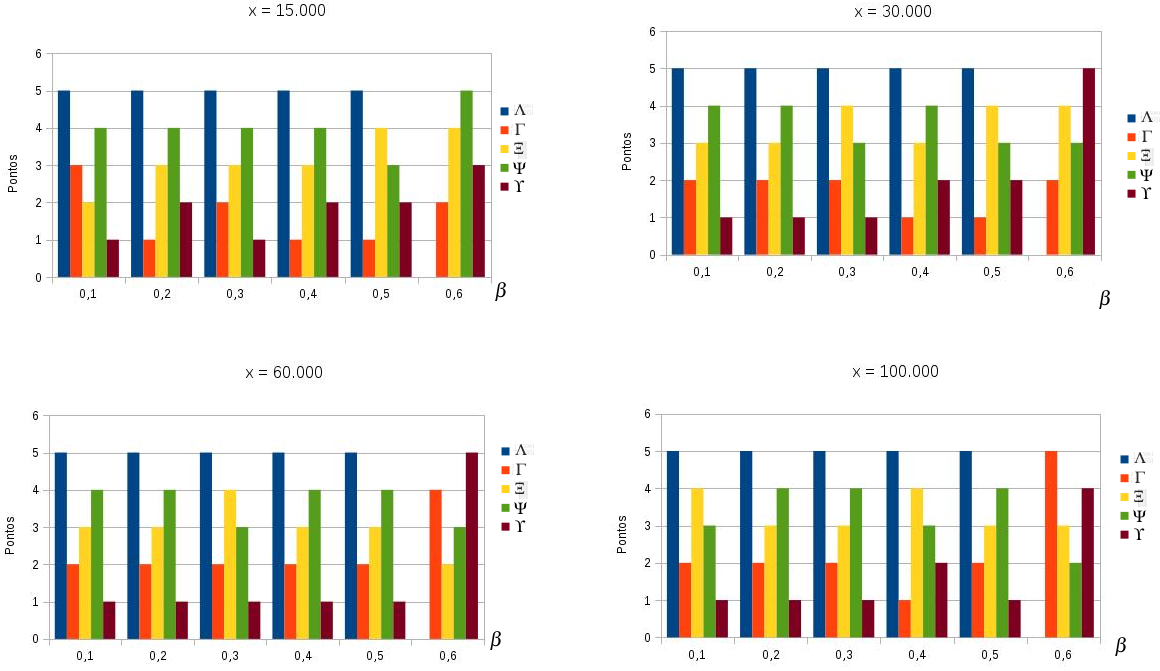
\includegraphics[width=300pt]{imagens_resultados/total_vertices.png}
  \caption{\footnotesize{Pontuação referente ao total de vértices para malhas com $\chi = 15.000$, $\chi = 30.000$, $\chi = 60.000$ e $\chi = 100.000$, com $\beta = 0,1$,
 $\beta = 0,2$, $\beta = 0,3$, $\beta = 0,4$, $\beta = 0,5$ e $\beta = 0,6$.
 \label{grafico_total_vertices}
}}
\end{figure}

\begin{figure}[!ht]
  \centering
  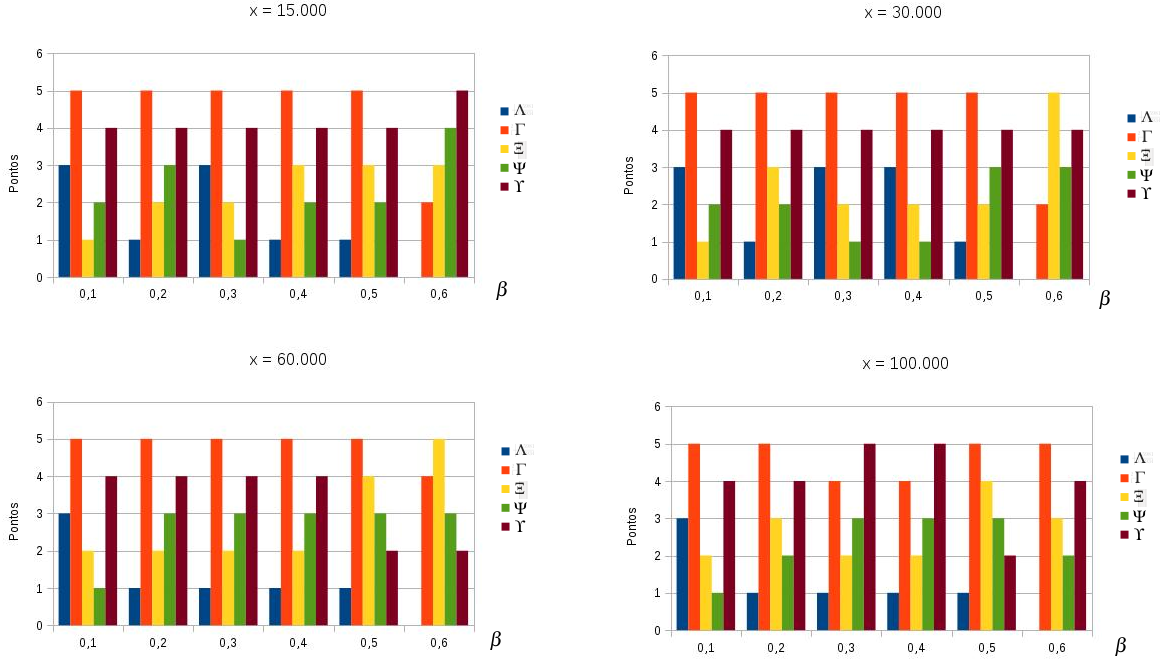
\includegraphics[width=300pt]{imagens_resultados/total_clocks.png}
  \caption{\footnotesize{Pontuação referente ao total de {\it clocks} para malhas com $\chi = 15.000$, $\chi = 30.000$, $\chi = 60.000$ e $\chi = 100.000$, com $\beta = 0,1$, $\beta = 0,2$, $\beta = 0,3$, $\beta = 0,4$, $\beta = 0,5$ e $\beta = 0,6$.
   \label{grafico_total_clocks}
}}
\end{figure}

\begin{figure}[!ht]
  \centering
  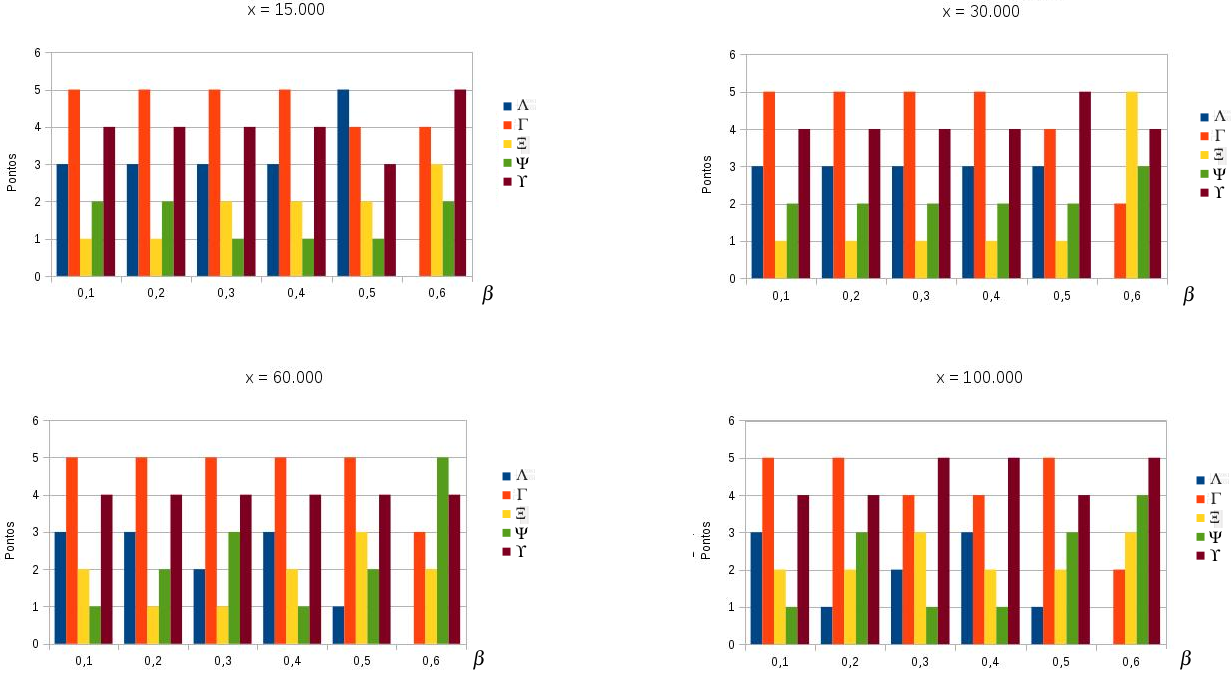
\includegraphics[width=300pt]{imagens_resultados/clocks_mov.png}
  \caption{\footnotesize{Pontuação referente ao total de {\it clocks} para movimentar os vértices, para malhas com $\chi = 15.000$, $\chi = 30.000$, $\chi = 60.000$ e $\chi = 100.000$, com $\beta = 0,1$, $\beta = 0,2$, $\beta = 0,3$, $\beta = 0,4$, $\beta = 0,5$ e $\beta = 0,6$.
   \label{grafico_total_mov}
}}
\end{figure}

\begin{figure}[!ht]
  \centering
  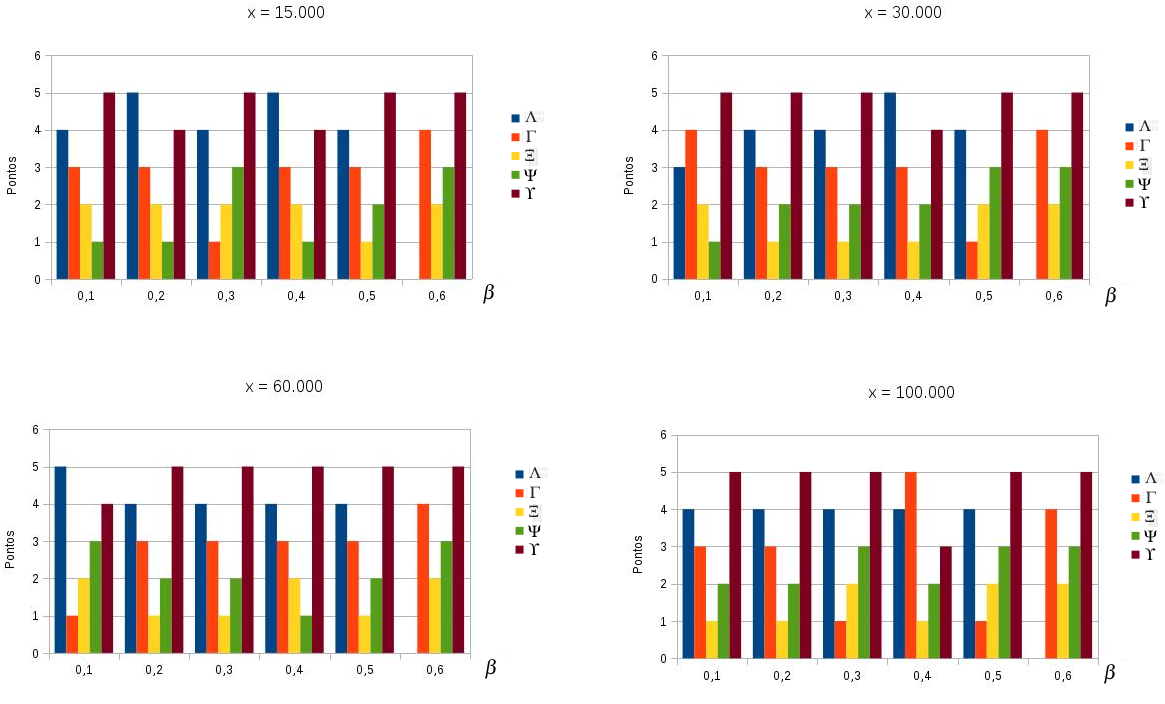
\includegraphics[width=300pt]{imagens_resultados/gamma_max.png}
  \caption{\footnotesize{Pontuação referente ao valor de $\gamma_{max}$, para malhas com $\chi = 15.000$, $\chi = 30.000$, $\chi = 60.000$ e $\chi = 100.000$, com $\beta = 0,1$, $\beta = 0,2$, $\beta = 0,3$, $\beta = 0,4$, $\beta = 0,5$ e $\beta = 0,6$.
   \label{grafico_gamma_max}
}}
\end{figure}

\begin{figure}[!ht]
  \centering
  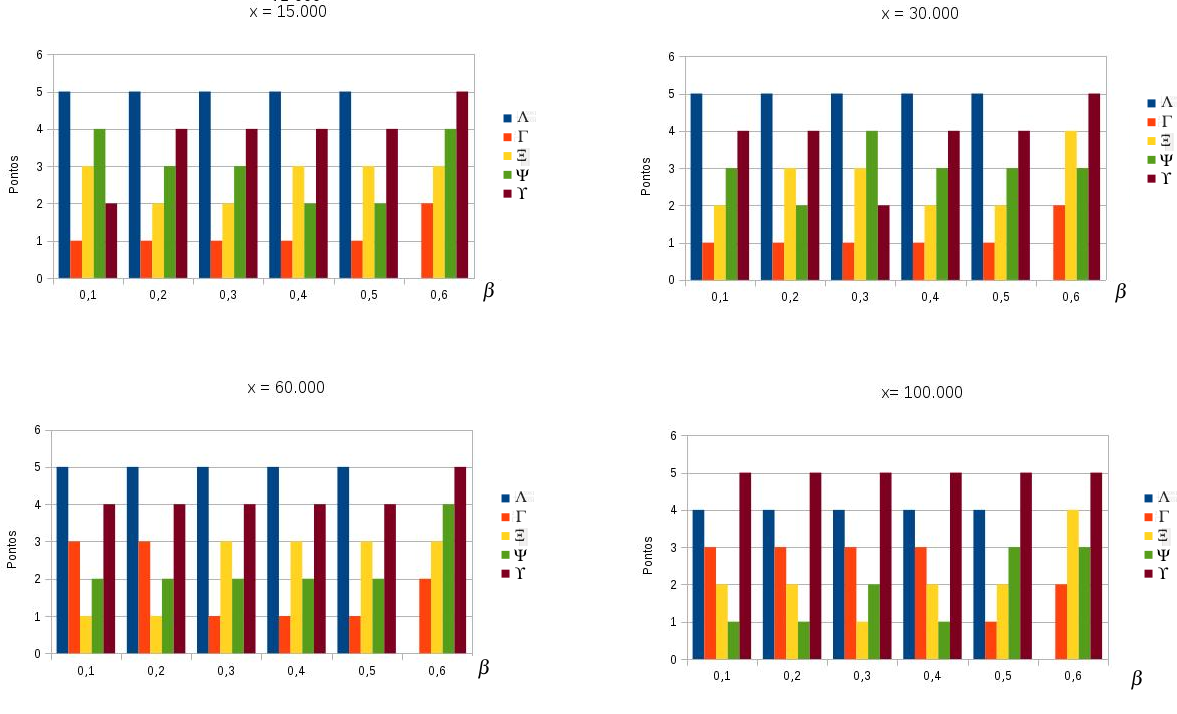
\includegraphics[width=300pt]{imagens_resultados/gamma_mean.png}
  \caption{\footnotesize{Pontuação referente ao valor de $\gamma_{mean}$, para malhas com $\chi = 15.000$, $\chi = 30.000$, $\chi = 60.000$ e $\chi = 100.000$, com $\beta = 0,1$, $\beta = 0,2$, $\beta = 0,3$, $\beta = 0,4$, $\beta = 0,5$ e $\beta = 0,6$.
   \label{grafico_gamma_mean}
}}
\end{figure}

\begin{figure}[!ht]
  \centering
  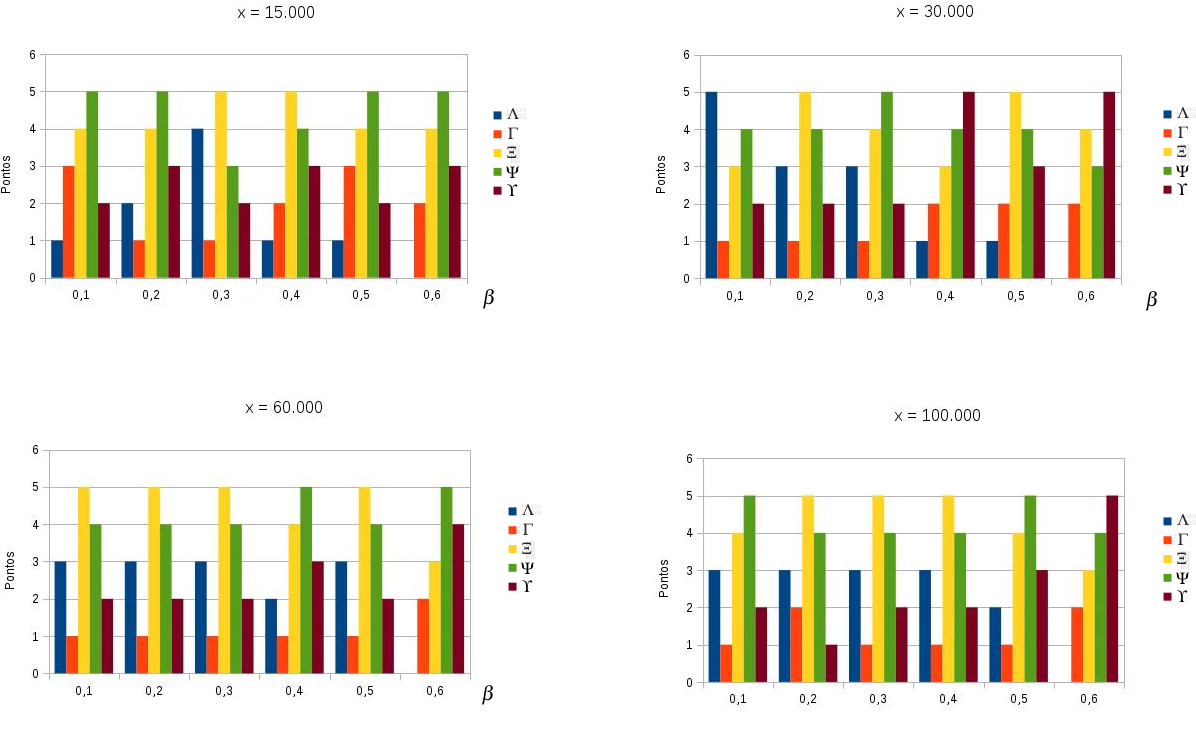
\includegraphics[width=300pt]{imagens_resultados/rho_max.png}
  \caption{\footnotesize{Pontuação referente ao valor de $\rho_{max}$, para malhas com $\chi = 15.000$, $\chi = 30.000$, $\chi = 60.000$ e $\chi = 100.000$, com $\beta = 0,1$, $\beta = 0,2$, $\beta = 0,3$, $\beta = 0,4$, $\beta = 0,5$ e $\beta = 0,6$.
   \label{grafico_rho_max}
}}
\end{figure}

\begin{figure}[!ht]
  \centering
  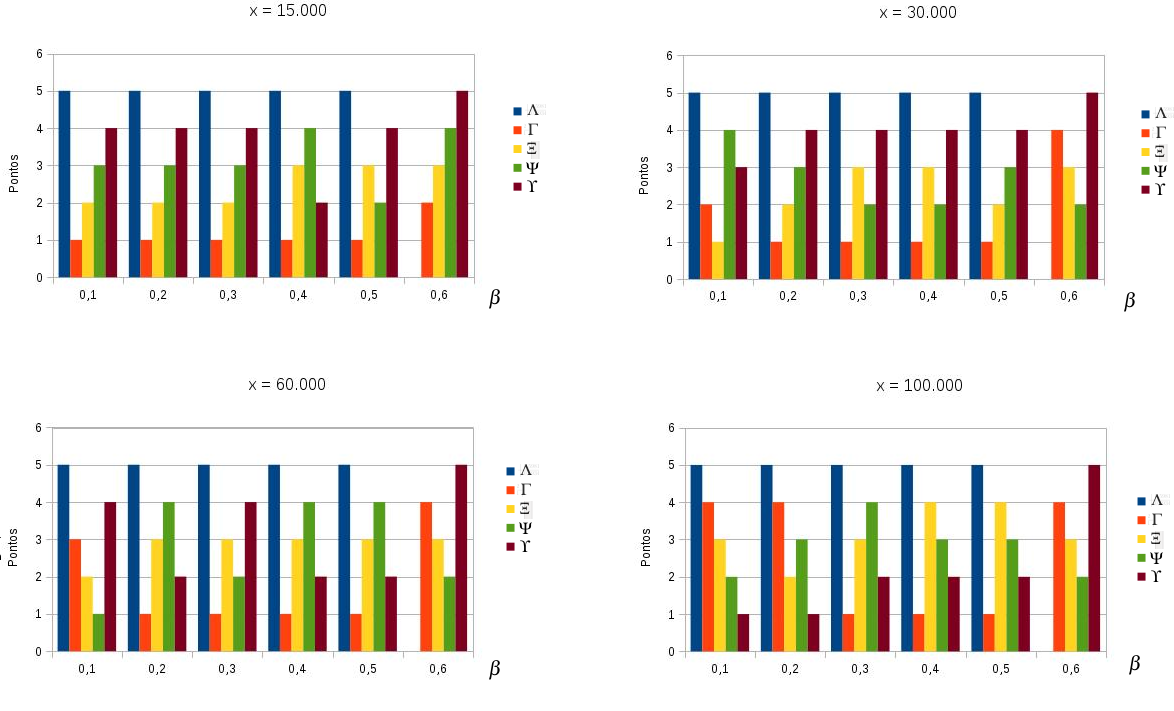
\includegraphics[width=300pt]{imagens_resultados/per_rho.png}
  \caption{\footnotesize{Pontuação referente à porcentagem de triângulos com $\rho > \rho_{\alpha}$, para malhas com $\chi = 15.000$, $\chi = 30.000$, $\chi = 60.000$ e $\chi = 100.000$, com $\beta = 0,1$, $\beta = 0,2$, $\beta = 0,3$, $\beta = 0,4$, $\beta = 0,5$ e $\beta = 0,6$.
   \label{grafico_per_rho}
}}
\end{figure}

\begin{figure}[!ht]
  \centering
  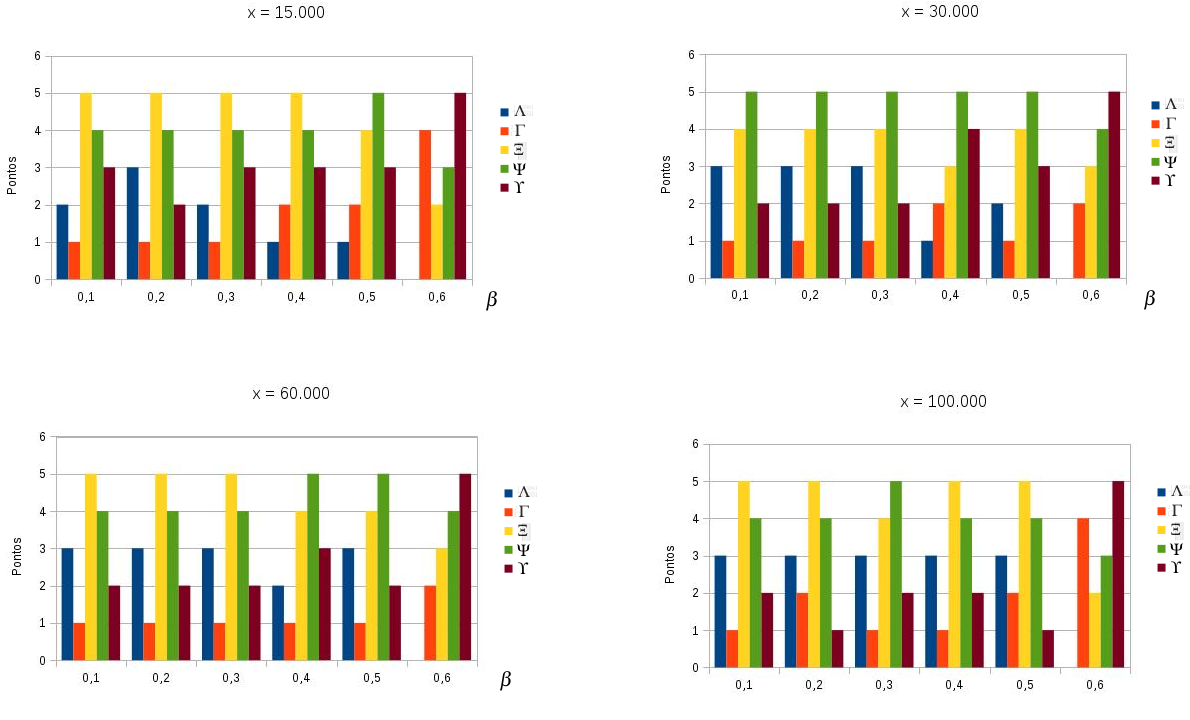
\includegraphics[width=300pt]{imagens_resultados/upsilon_min.png}
  \caption{\footnotesize{Pontuação referente ao valor de $\upsilon_{min}$, para malhas com $\chi = 15.000$, $\chi = 30.000$, $\chi = 60.000$ e $\chi = 100.000$, com $\beta = 0,1$, $\beta = 0,2$, $\beta = 0,3$, $\beta = 0,4$, $\beta = 0,5$ e $\beta = 0,6$.
   \label{grafico_upsilon_min}
}}
\end{figure}

\begin{figure}[!ht]
  \centering
  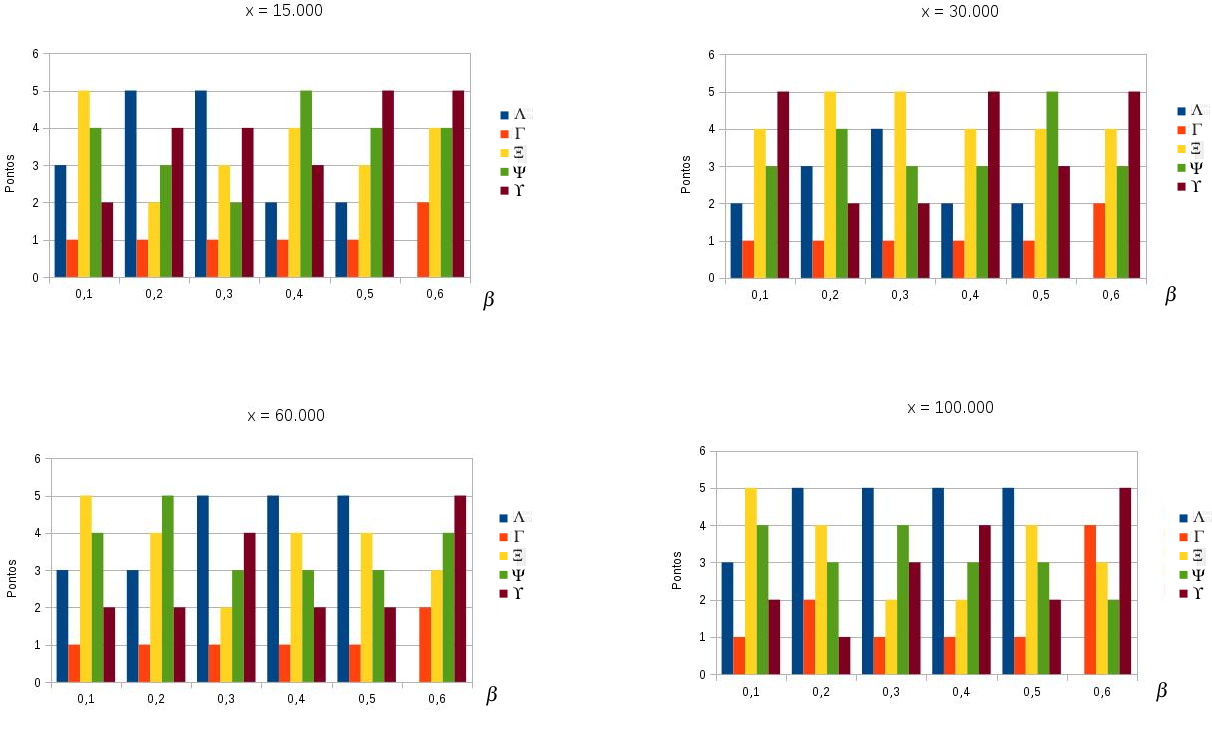
\includegraphics[width=300pt]{imagens_resultados/per_upsilon.png}
  \caption{\footnotesize{Pontuação referente à porcentagem de triângulos com $\upsilon < \eta$, para malhas com $\chi = 15.000$, $\chi = 30.000$, $\chi = 60.000$ e $\chi = 100.000$, com $\beta = 0,1$, $\beta = 0,2$, $\beta = 0,3$, $\beta = 0,4$, $\beta = 0,5$ e $\beta = 0,6$.
   \label{grafico_per_upsilon}
}}
\end{figure}

\begin{figure}[!ht]
  \centering
  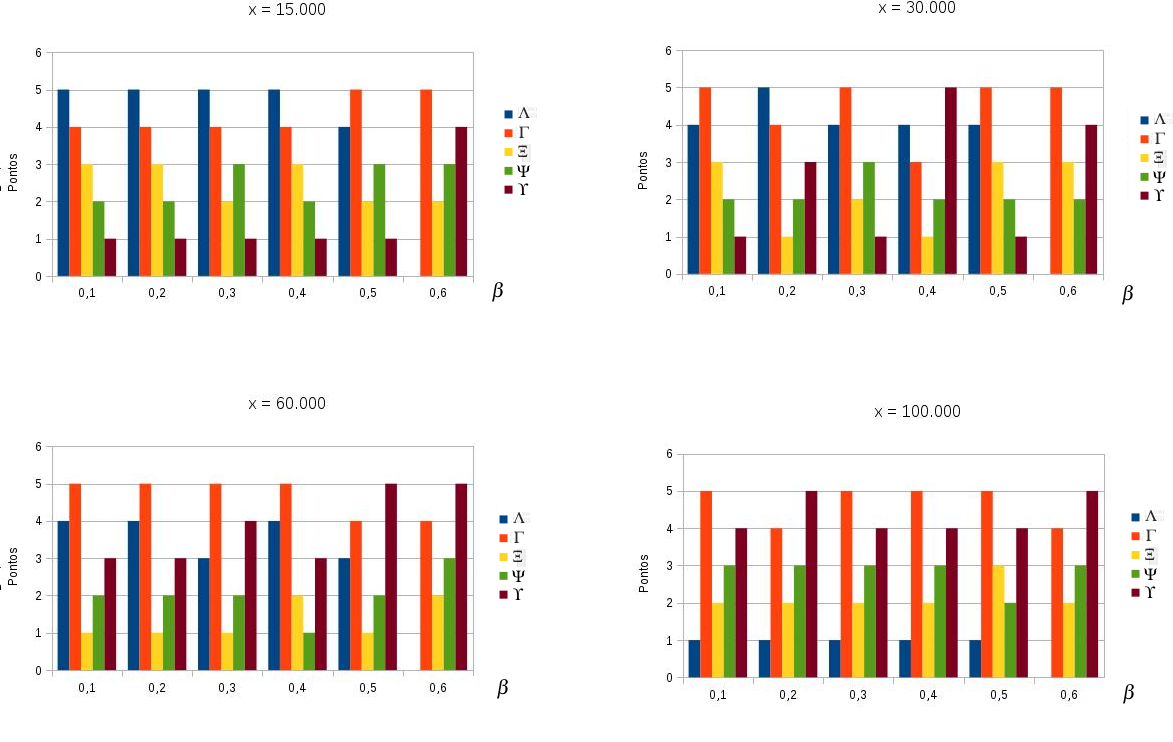
\includegraphics[width=300pt]{imagens_resultados/cresc_gamma.png}
  \caption{\footnotesize{Pontuação referente à porcentagem de crescimento de $\gamma_{mean}$, para malhas com $\chi = 15.000$, $\chi = 30.000$, $\chi = 60.000$ e $\chi = 100.000$, com $\beta = 0,1$, $\beta = 0,2$, $\beta = 0,3$, $\beta = 0,4$, $\beta = 0,5$ e $\beta = 0,6$.
   \label{grafico_cresc_gamma}
}}
\end{figure}
\section{CONCLUSÃO E PROPOSTAS DE TRABALHOS FUTUROS}
\label{cap:conclusao}

Neste trabalho, foi proposta uma nova função monitora, chamada de $\Lambda$, e comparou-se os resultados  obtidos com os resultados de outras funções monitoras encontradas na literatura. 

Classificaram-se as funções monitoras de acordo com cada critério analisado. Com os resultados obtidos, pode-se verificar que cada função monitora possui suas qualidades e deficiências. A função $\Gamma$ mostrou-se eficiente por apresentar movimentos rápidos, com baixo custo computacional. No entanto, também apresentou a maior degeneração da malha, com os piores valores das métricas  {\it Circunradius-to-shortest Edge Radio} (CER) e {\it Shape Regularity Quality} (SRQ), a maior percentagem de triângulos com as métricas CER e SRQ consideradas ruins, também necessitando de mais vértices para correção da malha. A funçao $\Lambda$ foi a que apresentou valores razoáveis, em comparação com as demais, do maior valor e do valor médio do gradiente, denotados, respectivamente, $\gamma_{max}$ e $\gamma_{mean}$. Porém, como deficiência, a função $\Lambda$ demandou maior custo computacional para execução.

Os experimentos com as funções $\Xi$ e $\Psi$ confirmaram que a principal qualidade dessas funções é a melhoria da qualidade da malha. Apresentaram os melhores resultados em relação às métricas CER e SRQ. Também apresentaram movimentos suaves, não ocorrendo grandes variações ao se utilizar diferentes parâmetros de adaptatividade, definido por $\beta$. Como deficiência, apresentaram baixos valores de $\gamma_{max}$ e $\gamma_{mean}$, ao se comparar com uma malha sem movimentar os vértices. Até a publicação deste trabalho, não foram encontrados outros trabalhos em que se utilizassem as funções de \citeonline[seção 3]{Taubin1995}, \citeonline[seção 2]{Taubin1995A} e \citeonline{Kobbelt1998} a fim de obter melhorias na aproximação da solução de equação diferencial parcial.

A função $\Upsilon$ apresentou valores razoáveis de $\gamma_{max}$ e $\gamma_{mean}$, com custo computacional relativamente baixo. Entretanto, em vários experimentos utilizando essa função, as malhas apresentaram a maior quantidade de vértices em relação às demais. 

Para o usuário que deseja movimento dos vértices da malha, com altos valores de $\gamma_{max}$ e $\gamma_{mean}$, sem necessidade de inclusão de vértices para melhoria da malha, a função $\Lambda$ pode ser a melhor alternativa. Ainda, para o usuário que deseja boa qualidade da malha nas métricas CER e SRQ, as funções $\Xi$  e $\Psi$ podem ser excelentes alternativas.

Para o usuário que deseja custo computacional baixo e gradientes razoáveis na malha, a função $\Gamma$ é uma boa alternativa em relação às funções $\Lambda$ e $\Upsilon$, desde que não haja problemas na inclusão de vértices para melhoria na malha.

A função $\Upsilon$ é interessante para usuários que desejam altos valores de $\gamma_{max}$, com taxa de crescimento do gradiente relativamente baixa, sem se importar com a inclusão de vértices para melhoria da qualidade da malha.

É importante salientar que o movimento dos vértices não deve ser utilizado sem análise e planejamento. Em todos os experimentos, ocorreu que movimentar os vértices acarretou um custo computacional maior que realizar somente o refinamento da malha. É possível que o custo de movimentar os vértices possa ser reduzido aumentando-se a intensidade do movimento e, consequentemente, reduzindo o número de iterações das linhas \ref{laco_repita_inicio}-\ref{laco_repita_fim} do algoritmo (\ref{malha_movel}). Os testes com ``S/Mov.2'' resultam em malhas com a qualidade mínima estipulada pelo usuário. Isso significa que os testes com ``S/Mov.2'' resultam em malhas de qualidade. Em todos os testes realizados, ``S/Mov.2'' resultou em menor custo computacional.

Como melhoria neste trabalho, seria importante realizar pesquisas sobre estimadores de erros {\it a posteriori}, equação do calor com termo fonte ou mesmo a aplicação em outra equação para análise e verificação da solução gerada. 

Ainda, como proposta de trabalho futuro, seria a adaptação para discretizações de volumes finitos dos esquemas de movimentos de malhas de discretizações de elementos finitos baseados em \citeonline{Huang2011}. Ainda, os esquemas propostos por \citeonline{Springel2009} podem ser boas alternativas para a implementação de malhas móveis para se manter a qualidade da malha com baixo custo computacional na solução de equações diferenciais parciais.

Com o intuito de se reduzir o tempo de processamento dos experimentos, bem como obter uma solução com melhor aproximação e em tempo hábil, também necessita-se paralelizar o método dos gradientes conjugados, método que mais demanda recursos de processamento.

Com relação à malha, pode-se realizar experimentos com diferentes valores de fronteira e/ou com um domínio com geometria complexa. Também é possível obter melhorias nos resultados aumentando o parâmetro de adaptatividade $\beta$, ou mesmo, utilizando um $\beta$ local.

\vfill\null\newpage
\renewcommand{\baselinestretch}{1.0}
\bibliographystyle{abntex2-alf}
 \bibliografia{referencias}

% \renewcommand{\baselinestretch}{1.0}\normalsize
% \def\hyphenpenalty{10000}
% \def\exhyphenpenalty{10000}
% \refstitle{REFERÊNCIAS}
% \providecommand{\abntreprintinfo}[1]{%
%  \citeonline{#1}}
% \setlength{\labelsep}{0pt}\begin{thebibliography}{}
% \providecommand{\abntrefinfo}[3]{}
% \providecommand{\abntbstabout}[1]{}
% \abntbstabout{v-1.9 }
% \normalsize\normalfont
% \setlength{\itemsep}{16pt}
% 
% 
% 
% 
% 
% 
% \end{thebibliography}

% Apendices e anexos
% \newpage
% \apendices
% %\input{sections/apend-middleware}
% \apendice{Primeiro Apêndice}
% Texto.

% \newpage
% \apendice{Segundo Apêndice}
% Texto.

% \newpage
% \anexos
% %\input{sections/apend-middleware}
% \anexo{Primeiro Anexo}
% Texto.

% \newpage
% \anexo{Segundo Anexo}
% Texto.

\end{document}
